% Created 2024-12-01 Sun 20:04
% Intended LaTeX compiler: pdflatex
\documentclass[11pt]{article}
\usepackage[utf8]{inputenc}
\usepackage[T1]{fontenc}
\usepackage{graphicx}
\usepackage{longtable}
\usepackage{wrapfig}
\usepackage{rotating}
\usepackage[normalem]{ulem}
\usepackage{amsmath}
\usepackage{amssymb}
\usepackage{capt-of}
\usepackage{hyperref}
\usepackage{minted}
\usepackage{siunitx}
\usepackage{array}
\setlength{\parindent}{0em}
\author{Hankertrix}
\date{\today}
\title{MA3010 Thermodynamics and Heat Transfer Cheat Sheet (Heat Transfer Section)}
\hypersetup{
 pdfauthor={Hankertrix},
 pdftitle={MA3010 Thermodynamics and Heat Transfer Cheat Sheet (Heat Transfer Section)},
 pdfkeywords={},
 pdfsubject={},
 pdfcreator={Emacs 29.4 (Org mode 9.6.15)}, 
 pdflang={English}}
\begin{document}

\maketitle
\setcounter{tocdepth}{2}
\tableofcontents \clearpage
\section{Definitions}
\label{sec:org33b3245}

\subsection{Heat}
\label{sec:org5d5c244}
\begin{itemize}
\item Heat is a form of \textbf{energy} stored by matter.
\item It is associated with the \textbf{microscopic movement} of individual particles, like molecular translation, rotation vibration, random motion, etc.
\end{itemize}

Other forms of energy include:

\begin{itemize}
\item Microscopic level
\begin{itemize}
\item Chemical energy (binding of molecules)
\item Electrical energy (binding between charged particles)
\item Atomic energy (binding between protons, neutrons and electrons)
\end{itemize}

\item Macroscopic level (organised / bulk motion)
\begin{itemize}
\item Kinetic energy (\(\frac{1}{2} mv^2\))
\item Potential energy (\(mgh\))
\end{itemize}
\end{itemize}

\subsection{Heat transfer}
\label{sec:org36229d0}
\begin{itemize}
\item Heat transfer is the transit of energy due to \textbf{temperature difference}.
\item Heat energy flows from \textbf{hot to cold} surfaces.
\item There are three modes of heat transfer:
\begin{itemize}
\item \textbf{Conduction}
\item \textbf{Convection}
\item \textbf{Radiation}
\end{itemize}
\item Units:
\begin{itemize}
\item Heat: Joules (\(\unit{J}\)), British thermal units (\(\unit{Btu}\)), calories (\(\unit{cal}\))
\item Rate of heat transfer: Watt (\(\unit{W}\)), British thermal units per hour (\(\unit{Btu.h^{-1}}\)), horsepower (\(\unit{hp}\))
\end{itemize}
\end{itemize}

\subsubsection{Simultaneous heat transfer mechanisms}
\label{sec:org9757d0f}
\begin{itemize}
\item Most cases of heat transfer in practical applications involve a combination of heat transfer modes between mediums.
\item However, not all three can exist simultaneously in a medium.
\begin{itemize}
\item Opaque solid: Conduction only
\item Fluid: Radiation and convection \textbf{or} conduction
\item Vacuum: Radiation only
\end{itemize}
\end{itemize}

\begin{center}
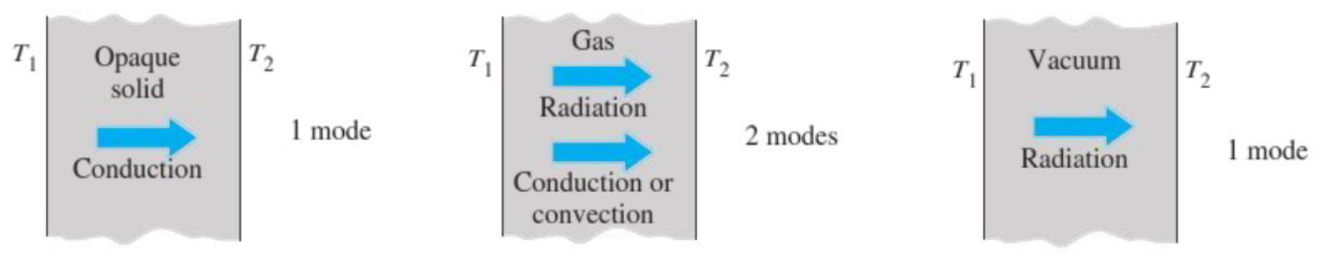
\includegraphics[width=.9\linewidth]{./images/simultaneous-heat-transfer-mechanisms.png}
\end{center}

\subsection{Conduction}
\label{sec:org4cc056a}
\begin{itemize}
\item Conduction is the diffusion of heat \textbf{from more energetic to adjacent less energetic particles} with \textbf{no net bulk motion} between the particles.
\item Conduction flows through solids or stationary fluids.
\item Conduction in a fluid is a \textbf{limiting case} of convection.
\end{itemize}

 \newpage

\subsubsection{Fourier's law of conduction}
\label{sec:org3ae2c07}
\[\dot{Q} = -kA \frac{dT}{dx}\]
\[\dot{Q} = -kA \frac{dT}{dr}\]
\[\dot{Q} = -kA \frac{T_2 - T_1}{L}\]

Where:
\begin{itemize}
\item \(\dot{Q}\) is the rate of heat transfer (\(\unit{W}\))
\item \(A\) is the area \textbf{perpendicular} to the heat flow direction (\(\unit{m^2}\))
\item \(\frac{dT}{dx}\) is the temperature gradient \textbf{along heat flow direction} in Cartesian coordinates (\(\unit{K.m^{-1}}\))
\item \(\frac{dT}{dr}\) is the temperature gradient \textbf{along heat flow direction} in polar or cylindrical coordinates (\(\unit{K.m^{-1}}\))
\item \(k\) is the thermal conductivity of the medium (\(\unit{W.m^{-1}.K^{-1}}\))
\item \(T_2\) is the temperature at the end of the heat flow
\item \(T_1\) is the initial temperature at the start of the heat flow
\item \(L\) is the length the heat has to flow through
\end{itemize}

\subsection{Thermal conductivity (\(k\))}
\label{sec:org238cd29}
\begin{itemize}
\item Thermal conductivity is a measure of a material's ability to conduct heat.
\begin{itemize}
\item Material property (\(\unit{W.m^{-1}.K^{-1}}\))
\item A high value of \(k\) means the material is a good heat conductor
\item A low value of \(k\) means the material is an insulator of heat
\end{itemize}
\item The value of a material's thermal conductivity varies with temperature, i.e. \(k(T)\).
\begin{itemize}
\item For solids and liquids: no fixed trend for the variation of a material's conductivity with temperature.
\item For gases, thermal conductivity increases with temperature.
\end{itemize}
\item The thermal conductivity of various materials can be found table 1-1 of the property tables.
\end{itemize}

\subsection{Heat generation}
\label{sec:orgdc5835b}
\begin{itemize}
\item Heat generation is the \textbf{conversion} of other types of \textbf{energy} (mechanical, electrical, chemical, etc.) \textbf{into heat} within a medium.
\item Heat generation is a \textbf{volumetric phenomenon}:
\[\dot{e}_{gen} (x, y, z, t), \quad \unit{W.m^{-3}}\]
\item Total heat generation rate:
\[\dot{E}_{gen} = \int_V \dot{e}_{gen} dV \quad (\unit{W})\]
\item For \textbf{uniform} heat generation, \(\dot{e}_{gen} = \text{constant}\):
\[\dot{E}_{gen} = \dot{e}_{gen} V \quad (\unit{W})\]
\end{itemize}

\subsection{One-dimensional heat conduction (Formula given)}
\label{sec:org7c015c1}
\begin{itemize}
\item Heat conduction in most cases can be approximated as being one-dimensional
\begin{itemize}
\item One dominant direction for heat transfer
\item Negligible or no heat transfer in other directions.
\end{itemize}
\end{itemize}

\subsubsection{Derivation}
\label{sec:orgcc8ad20}
\textbf{Diagram:}
\begin{center}
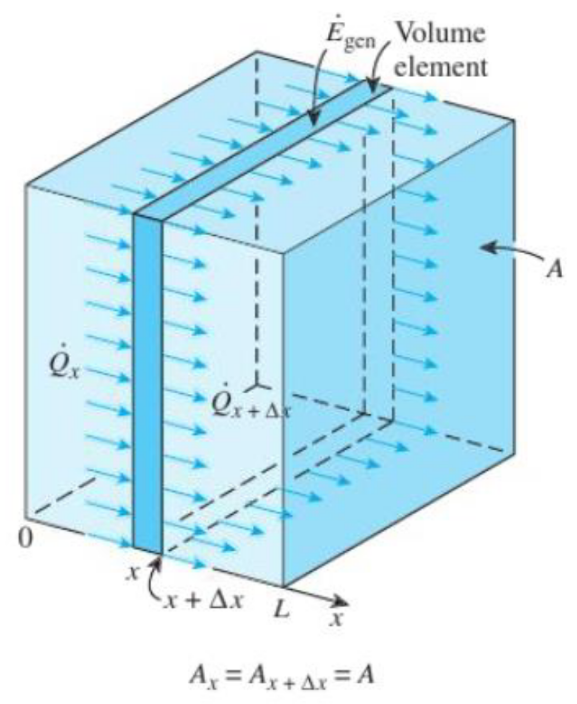
\includegraphics[scale=0.5]{./images/one-dimensional-heat-conduction.png}
\end{center}

\textbf{Details:}
\begin{itemize}
\item Energy balance for the "slice" of the volume element:
\end{itemize}
\begin{center}
\begin{tabular}{>{\centering\arraybackslash}m{7em} >{\centering\arraybackslash}m{1em} >{\centering\arraybackslash}m{7em} >{\centering\arraybackslash}m{1em} >{\centering\arraybackslash}m{7em} >{\centering\arraybackslash}m{1em} >{\centering\arraybackslash}m{7em}}
Rate of heat conduction at \(x\) & \(-\) & Rate of heat conduction at \(x + \Delta x\) & \(+\) & Rate of heat generation inside the element & \(=\) & Rate of energy change of the element\\[0pt]
\(\dot{Q}_x\) & \(-\) & \(\dot{Q}_{x + \Delta x}\) & \(+\) & \(\dot{E}_{\text{gen, element}}\) & \(=\) & \(\frac{\Delta E_{element}}{\Delta t}\)\\[0pt]
\end{tabular}
\end{center}

\begin{itemize}
\item For uniform rate of energy generation:
\[\dot{E}_{\text{gen, element}} = \dot{e}_{gen} V_{element} = \dot{e}_{gen} A \Delta x\]
\item Change in energy of the element:
\begin{align*}
\Delta E_{element} &= E_{t + \Delta x} - E_t \\
&= mC(T_{t + \Delta t} - T_t) \\
&= \rho A \Delta x C (T_{t + \Delta t} - T_t)
\end{align*}
\item Substituting:
\[\dot{Q}_x - \dot{Q}_{x + \Delta x} + \dot{e}_{gen} A \Delta x = \rho A \Delta x C \frac{(T_{t + \Delta t} - T_t)}{\Delta t}\]
\item Divide by \(A \Delta x\):
\[-\frac{1}{A} \frac{\dot{Q}_{x + \Delta x} - \dot{Q}_x}{\Delta x} + \dot{e}_{gen} = \rho C \frac{(T_{t + \Delta t} - T_t)}{\Delta t}\]
\item Taking the limit as \(\Delta x \rightarrow 0\) and \(\Delta t \rightarrow 0\):
\[-\frac{1}{A} \frac{\partial \dot{Q}}{\partial x} + \dot{e}_{gen} = \rho C \frac{\partial T}{\partial t}\]
\item Substituting Fourier's law of conduction, \(\dot{Q} = -kA \frac{\partial T}{\partial x}\):
\[\frac{1}{A} \frac{\partial}{\partial x} \left(kA \frac{\partial T}{\partial x} \right) + \dot{e}_{gen} = \rho C \frac{\partial T}{\partial t}\]
\item Since cross-sectional area is constant:
\[\frac{\partial}{\partial x} \left[k(T) \frac{\partial T}{\partial x} \right] + \dot{e}_{gen} = \rho C \frac{\partial T}{\partial t}\]
\item If thermal conductivity \(k\) is assumed to be constant:
\[k \frac{\partial^2 T}{\partial x^2} + \dot{e}_{gen} = \rho C \frac{\partial T}{\partial t} \quad (\text{Formula given in exam})\]
\end{itemize}

\subsubsection{Special cases in Cartesian coordinates}
\label{sec:orgadfa13b}
\begin{itemize}
\item Steady-state:
\[\frac{\partial T}{\partial t} = 0\]
\[k \frac{d^2 T}{dx^2} + \dot{e}_{gen} = 0\]
\item Steady-state, no heat generation:
\[\frac{\partial T}{\partial t} = 0, \quad \dot{e}_{gen} = 0\]
\[\frac{d^2 T}{dx^2} = 0\]
\item Transient, no heat generation:
\[\dot{e}_{gen} = 0\]
\[k \frac{d^2 T}{dx^2} = \rho C \frac{\partial T}{\partial t}\]
\end{itemize}

\subsubsection{Cylindrical coordinates}
\label{sec:org8d8438f}
\begin{itemize}
\item In Cartesian coordinates:
\[\frac{1}{A} \frac{\partial}{\partial x} \left(\frac{\partial T}{\partial x} \right) + \dot{e}_{gen} = \rho C \frac{\partial T}{\partial t}\]
\item Similarly, in cylindrical coordinates:
\[\frac{1}{A} \frac{\partial}{\partial r} \left(\frac{\partial T}{\partial r} \right) + \dot{e}_{gen} = \rho C \frac{\partial T}{\partial t}\]
\item Substituting the expression \(A = 2 \pi r L\):
\[\frac{1}{2 \pi r L} \frac{\partial}{\partial r} \left(2k \pi r L \frac{\partial T}{\partial r} \right) + \dot{e}_{gen} = \rho C \frac{\partial T}{\partial t}\]
\item Eliminating the common terms \(2 \pi L\):
\[\frac{1}{r} \frac{\partial}{\partial r} \left[k(T) r \frac{\partial T}{\partial r} \right] + \dot{e}_{gen} = \rho C \frac{\partial T}{\partial t}\]
\end{itemize}

\subsubsection{Special cases in cylindrical coordinates}
\label{sec:org0d3b8c0}
\begin{itemize}
\item Constant \(k\), steady-state:
\[\frac{\partial T}{\partial t} = 0\]
\[\frac{k}{r} \frac{\partial}{\partial r} \left(r \frac{\partial T}{\partial r} \right) + \dot{e}_{gen} = 0\]
\item Constant \(k\), steady-state, no heat generation:
\[\frac{\partial T}{\partial t} = 0, \quad \dot{e}_{gen} = 0\]
\[\frac{\partial}{\partial r} \left(r \frac{\partial T}{\partial r} \right) = 0\]
\item Constant \(k\), transient, no heat generation:
\[\dot{e}_{gen} = 0\]
\[\frac{k}{r} \frac{\partial}{\partial r} \left(r \frac{\partial T}{\partial r} \right) = \rho C \frac{\partial T}{\partial t}\]
\end{itemize}

\subsection{Internal heat generation}
\label{sec:orgd277454}
\begin{itemize}
\item Practical applications may involve the conversion of energy into thermal energy within the medium, which is heat generation
\begin{itemize}
\item Resistance heating in wires
\item Exothermic chemical reactions in a solid
\item Nuclear reactions in fuel rods
\end{itemize}
\item Heat generation (\(\dot{e}_{gen}\)) is expressed as \textbf{per unit volume} of the medium.
\end{itemize}

 \newpage

\subsubsection{Heat generation from electrical resistance heating}
\label{sec:org440e27f}
\[\dot{e}_{gen} = \frac{\dot{E}_{gen}}{V} = \frac{I^2 R_e}{\pi r_o^2 L} \quad (\unit{W.m^{-3}})\]

Where:
\begin{itemize}
\item \(\dot{E}_{gen}\) is the electrical power (\(\unit{W}\))
\item \(V\) is the volume of the wire in (\(\unit{m^3}\))
\item \(I\) is the current (\(\unit{A}\))
\item \(R_e\) is the electrical resistance (\(\unit{\ohm}\))
\item \(r_o\) is the outer radius of the wire
\item \(L\) is the length of the wire
\item \(\dot{e}_{gen}\) is the volumetric heat generation rate (\(\unit{W.m^{-3}}\))
\end{itemize}

 \newpage

\subsection{Steady internal heat generation}
\label{sec:org475ca22}
\begin{itemize}
\item Considering steady-state conditions, heat generated is transferred out of the solid at the same rate:
\begin{center}
\begin{tabular}{>{\centering\arraybackslash}m{12em} >{\centering\arraybackslash}m{1em} >{\centering\arraybackslash}m{12em}}
Rate of \textbf{heat generation} inside the solid & \(=\) & Rate of \textbf{heat transfer from the solid}\\[0pt]
\(\dot{E}_{gen} = \dot{e}_{gen} V\) & \(=\) & \(\dot{Q}\)\\[0pt]
\end{tabular}
\end{center}
\item In the event that heat is lost to the surroundings through convection heat transfer only:
\[\dot{Q} = h A_s (T_s - T_{\infty})\]
\[\dot{e}_{gen} V = h A_s (T_s - T_{\infty})\]
\[T_s = T_{\infty} + \frac{\dot{e}_{gen} V}{h A_s}\]
\[k \frac{\partial^2 T}{\partial x^2} + \dot{e}_{gen} = \rho C \frac{\partial T}{\partial t}\]
\item Steady state heat conduction equation:
\[\frac{\partial T}{\partial t} = 0\]
\[k \frac{\partial^2 T}{\partial x^2} + \dot{e}_{gen} = 0\]
\[\frac{\partial^2 T}{\partial x^2} + \frac{\dot{e}_{gen}}{k} = 0\]
\item Integrating twice:
\[T(x) = - \frac{\dot{e}_{gen}}{2k} x^2 + C_1 x + C_2\]
\item Needs two boundary conditions to solve the two constants of integration:
\[T(x = -L) = T_1, \qquad T(x = L) = T_2\]
\end{itemize}

 \newpage

\begin{itemize}
\item Use boundary conditions to solve for \(C_1\) and \(C_2\):
\begin{enumerate}
\item \(T(x = -L) = T_1\)
\[T_1 = - \frac{\dot{e}_{gen}}{2k} L^2 - C_1 L + C_2\]
\item \(T(x = L) = T_1\)
\[T_1 = - \frac{\dot{e}_{gen}}{2k} L^2 + C_1 L + C_2\]
\end{enumerate}
\[C_1 = \frac{T_2 - T_1}{2L}\]
\[C_2 = \frac{\dot{e}_{gen}}{2k} L^2 + \frac{T_1 + T_2}{2}\]
\item Temperature distribution:
\[T(x) = \frac{\dot{e}_g L^2}{2k} \left(1 - \frac{x^2}{L^2} \right) + \frac{T_2 - T_2}{2} \left(\frac{x}{L} \right) + \frac{T_1 + T_2}{2}\]
\end{itemize}

\subsubsection{Temperature distribution}
\label{sec:org4e3ab34}
\begin{center}
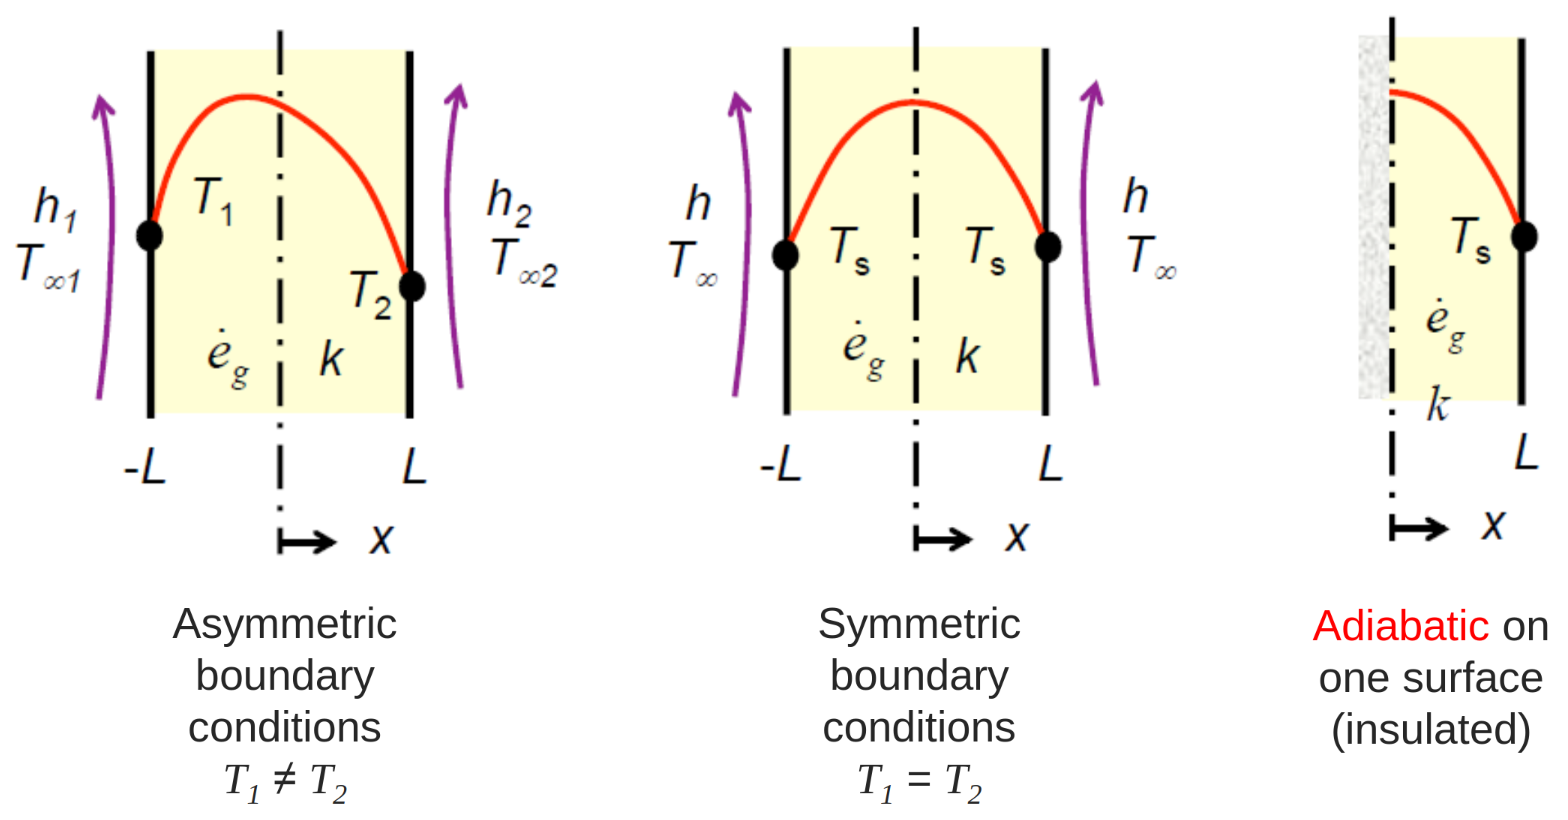
\includegraphics[width=.9\linewidth]{./images/steady-internal-heat-generation-temperature-distribution.png}
\end{center}

 \newpage

\subsubsection{Temperature distribution in cylinders}
\label{sec:orgb1f69d6}
\begin{itemize}
\item Steady-state heat conduction in cylindrical coordinates:
\[\frac{k}{r} \frac{d}{dr} \left(r \frac{dT}{dr} \right) + \dot{e}_{gen} = 0\]
\[\frac{1}{r} \frac{d}{dr} \left(r \frac{dT}{dr} \right) + \frac{\dot{e}_{gen}}{k} = 0 \quad (\text{Formula given in exam})\]
\item Integrating twice:
\[T(r) = - \frac{\dot{e}_{gen}}{4k} r^2 + C_1 \ln r + C_2\]
\item Boundary conditions:
\[T(r = r_o) = T_s\]
\[T(r = 0) = \text{finite}\]
\[\frac{dT}{dr}(r = 0) = 0 \quad (\text{Symmetry})\]
\item Use boundary conditions to solve for \(C_1\) and \(C_2\):
\begin{enumerate}
\item \(T(r = 0) = \text{finite}\):
\[T(r = 0) = C_1 \ln 0 + C_2\]
\[C_1 = 0\]
\item \(T(r= r_o) = T_s\):
\[T_s = - \frac{e\dot{e}_{gen}}{4k} r_o^2 + C_2\]
\[C_2 = T_s + \frac{\dot{e}_{gen} r_o^2}{4k}\]
\end{enumerate}
\item Temperature distribution:
\[T(r) = \frac{\dot{e}_{gen} r_o^2}{4k} \left(1 - \frac{r^2}{r_o^2} \right) + T_2\]
\end{itemize}

 \newpage

\subsection{Convection}
\label{sec:org3ad1dee}
\begin{itemize}
\item Convection is the transfer of heat through \textbf{bulk motion} of the fluid.
\item Convection requires the presence of a material (fluid) medium.
\item It is more complicated as it involves fluid motion and conduction.
\end{itemize}

\subsubsection{Newton's law of cooling}
\label{sec:org84c795b}
\[\dot{Q} = hA \Delta T\]

Where:
\begin{itemize}
\item \(h\) is the convective heat transfer coefficient (\(\unit{W.m^{-2}.K^{-1}}\))
\item \(A\) is the area through which heat is transferred
\item \(\Delta T\) is the temperature difference between bulk fluid temperature and surface temperature
\end{itemize}

\subsection{Radiation}
\label{sec:orgb388c2f}
Radiation is the energy emitted by matter in the form of electromagnetic waves (Maxwell) or photons (Planck).
\begin{itemize}
\item \textbf{No medium} is required for heat transmission
\item Any matter above absolute zero (\(\qty{0}{K}\)) emits electromagnetic radiation
\end{itemize}

\begin{center}
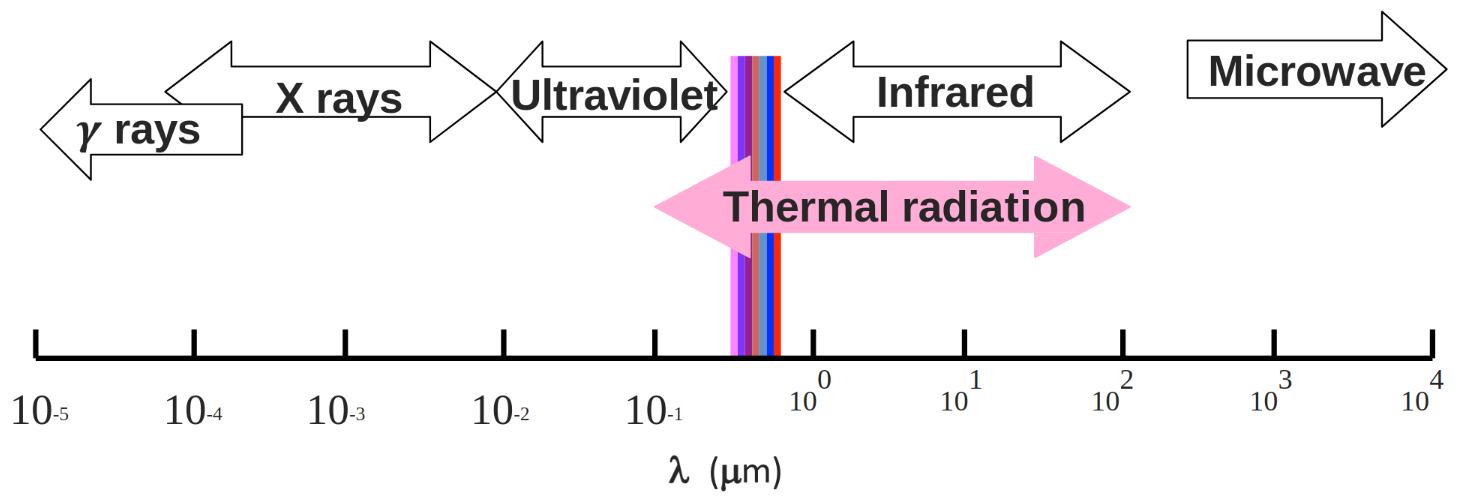
\includegraphics[width=.9\linewidth]{./images/electromagnetic-spectrum-for-thermal-radiation.png}
\end{center}

 \newpage

\subsection{Electromagnetic radiation}
\label{sec:org229949e}
\begin{itemize}
\item An idealised surface that emits \textbf{radiation} at the \textbf{max} rate is called a \textbf{blackbody}.
\item Rate of emission from a blackbody (the maximum possible rate) at \(T_s\) is given by the Stefan-Boltzmann Law of Radiation:
\[\dot{Q}_{\text{emit, max}} = \sigma A_s T_s^4\]

Where:
\begin{itemize}
\item \(\sigma\) is the Stefan-Boltzmann constant (\(5.670 \times 10^{-8} \ \unit{W.m^{-2}.K^{-4}}\))
\end{itemize}

\item All \textbf{real} surfaces emit \textbf{less} radiation than a blackbody at the same temperature:
\[\dot{Q}_{emit} = \varepsilon \sigma A_s T_s^4\]

Where:
\begin{itemize}
\item \(\varepsilon\) is the emissivity of the surface (\(0 \le \varepsilon \le 1\))
\end{itemize}
\end{itemize}

\subsubsection{Typical values of emissivity}
\label{sec:orgbbf25dd}
\begin{center}
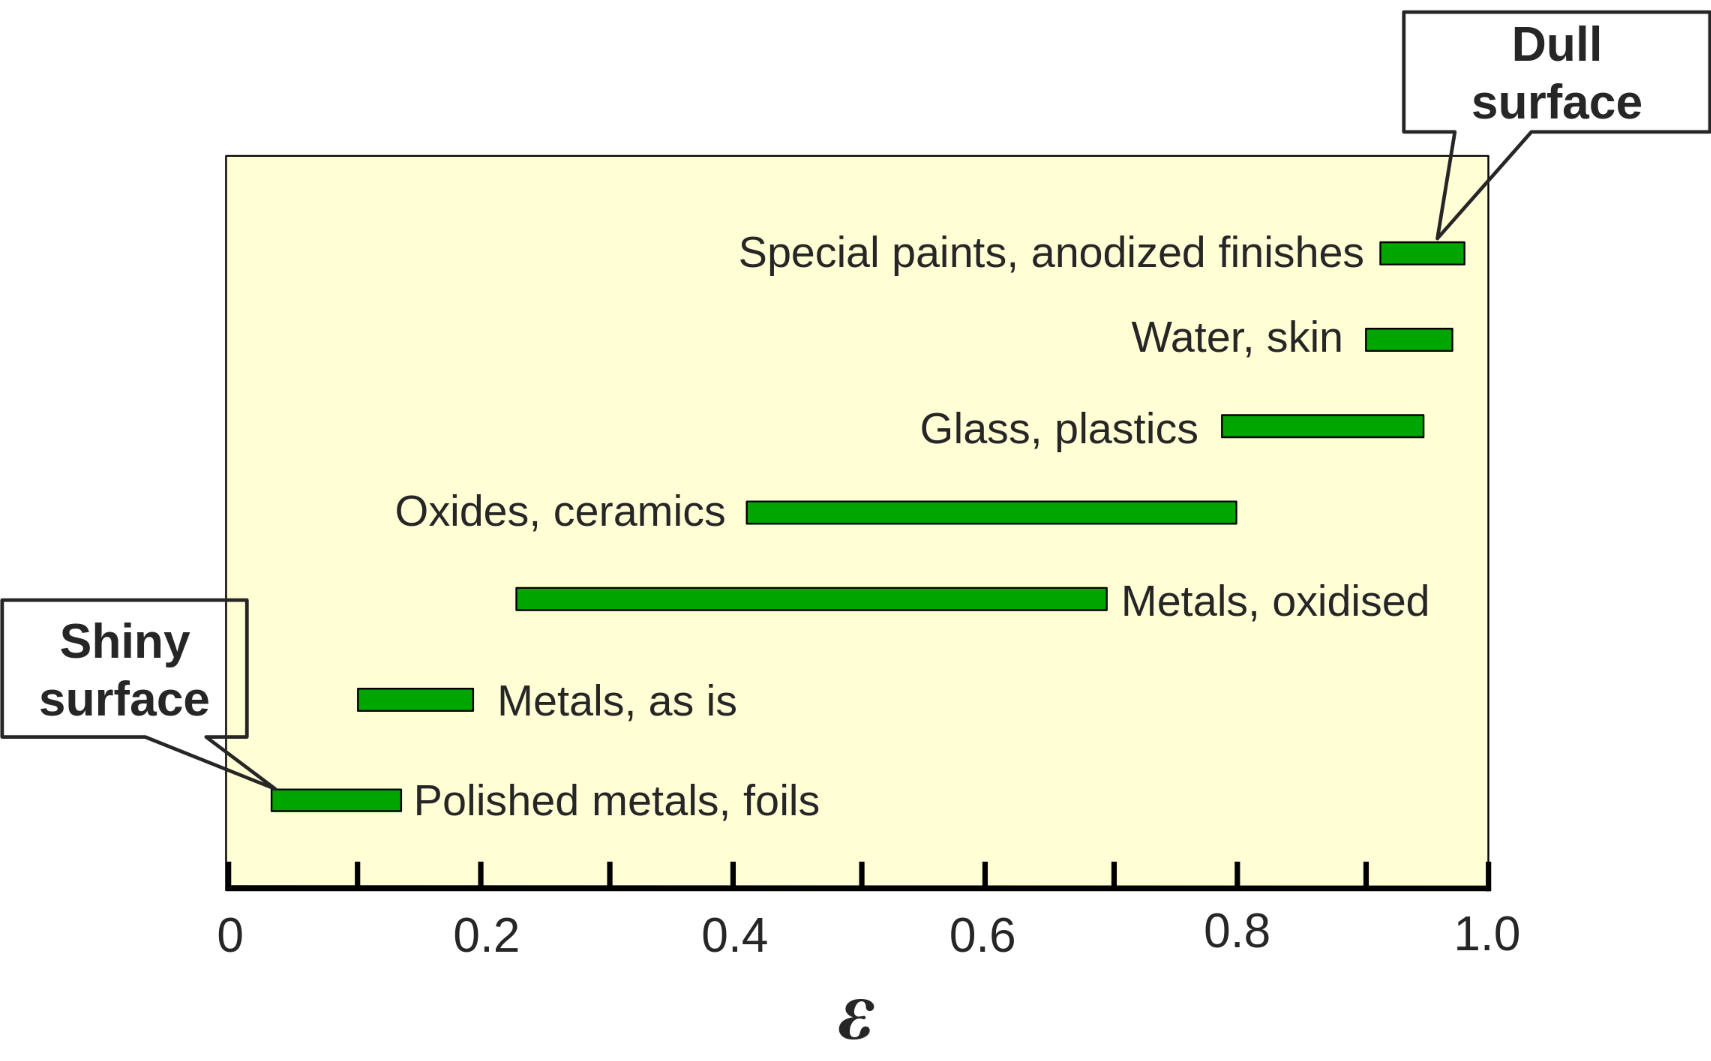
\includegraphics[width=.9\linewidth]{./images/typical-values-of-emissivity.png}
\end{center}

\subsubsection{Net radiation exchange}
\label{sec:orga681a31}
\begin{itemize}
\item Difference between the rates of radiation emission and radiation absorption for a surface is the net radiation heat exchange.
\begin{itemize}
\item Rate of emission > rate of absorption means heat is lost
\item Rate of emissions < rate of absorption means heat is gained
\end{itemize}
\item Radiation rate transfer between a surface and its surroundings:
\[\dot{Q}_{rad} = \dot{Q}_{emit} - \dot{Q}_{absorbed}\]
\[\dot{Q}_{rad} = \varepsilon \sigma A_s T_s^4 - \alpha \sigma A_s T_{surr}^4\]
\[\dot{Q}_{rad} = \varepsilon \sigma A_s \left(T_s^4 - T_{surr}^4 \right)\]
\end{itemize}

 \newpage

\subsection{Steady-state heat conduction}
\label{sec:org5949ba5}

\subsubsection{Plane wall}
\label{sec:org6431ee4}
\begin{center}
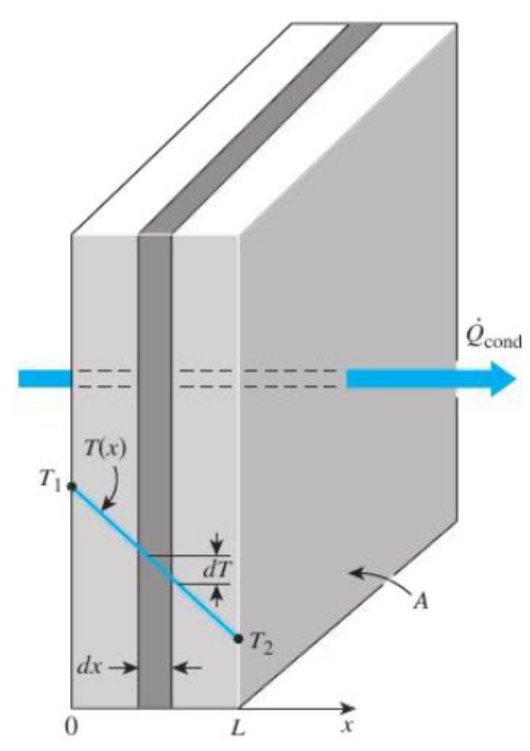
\includegraphics[scale=0.7]{./images/steady-state-heat-conduction-plane-wall.png}
\end{center}
\begin{itemize}
\item For steady-state heat conduction \textbf{with no heat generation}:
\[k \frac{\partial^2 T}{\partial x^2} + \dot{e}_{gen} = \rho C \frac{\partial T}{\partial t} \quad \rightarrow \quad \frac{d^2 T}{dx^2} = 0\]
\item Boundary conditions for a plane wall:
\[T(x = 0) = T_1 \quad T(x = L) = T_2\]
\item Integrate twice and applying boundary conditions would give the temperature distribution in the wall:
\[T = T_1 + (T_2 - T_1) \frac{x}{L}\]
\item Total heat transfer rate:
\[\dot{Q} = -kA \frac{dT}{dx} = -kA \frac{T_2 - T_1}{L} = kA \frac{\Delta T}{L}\]
\end{itemize}

\subsubsection{Hollow cylinder}
\label{sec:org16315ef}
\begin{center}
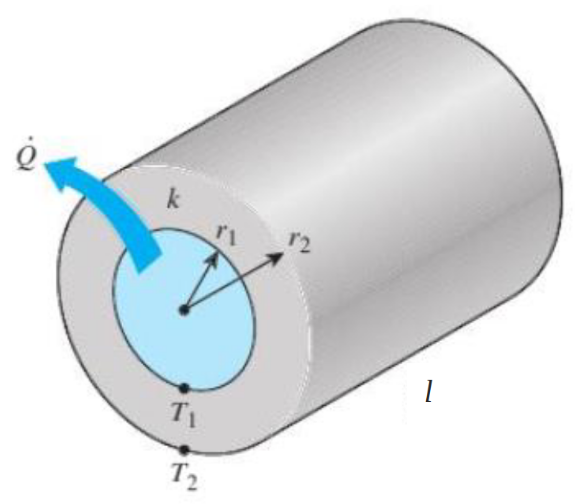
\includegraphics[width=.9\linewidth]{./images/steady-state-heat-conduction-hollow-cylinder.png}
\end{center}
\begin{itemize}
\item For steady-state heat conduction with \textbf{no heat generation}:
\[\frac{1}{r} \frac{\partial}{\partial r} \left[k(T) r \frac{\partial T}{\partial r} \right] + \dot{e}_{gen} = \rho C \frac{\partial T}{\partial t} \quad \rightarrow \quad \frac{\partial}{\partial r} \left(\frac{\partial T}{\partial r} \right) = 0\]
\item Boundary conditions for a hollow cylinder:
\[T(r = r_1) = T_1 \quad T(r = r_2) = T_2\]
\item Integrate twice and applying boundary conditions would give the temperature distribution:
\[T = T_2 + (T_1 - T_2) \left[\frac{\ln \left( \frac{r}{r_2} \right)}{\ln \left( \frac{r_1}{r_2} \right)} \right]\]
\item Total heat transfer rate:
\[\dot{Q} = -kA \frac{dT}{dr} = \frac{2 \pi kl (T_1 - T_2)}{\ln \left(\frac{r_2}{r_1} \right)}\]
\end{itemize}

\subsubsection{Hollow sphere (not tested)}
\label{sec:orgc01e971}
\begin{center}
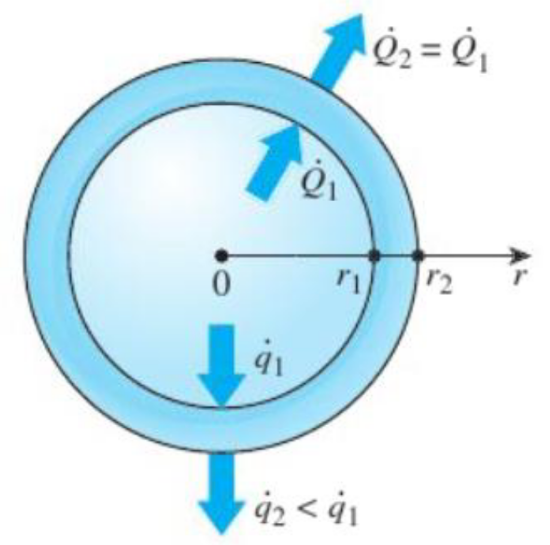
\includegraphics[width=.9\linewidth]{./images/steady-state-heat-conduction-hollow-sphere.png}
\end{center}
\begin{itemize}
\item Heat transfer rate is constant
\item Heat flux decreases due to increasing area
\item Temperature distribution in a hollow sphere:
\[T = T_1 + (T_2 - T_1) \frac{1 - \left(\frac{r_1}{r} \right)}{1 - \left(\frac{r_1}{r_2} \right)}\]
\item Total heat transfer rate:
\[\dot{Q} = \frac{4 \pi k (T_1 - T_2)}{\frac{1}{r_1} - \frac{1}{r_2}}\]
\end{itemize}

\subsection{Electrical resistance analogy}
\label{sec:orge9eb20f}
\begin{center}
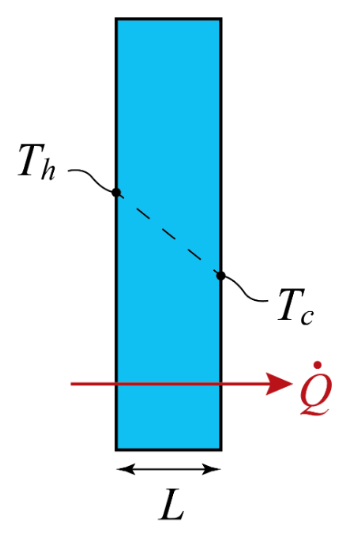
\includegraphics[scale=0.7]{./images/steady-state-heat-conduction-fouriers-law.png}
\end{center}
\begin{itemize}
\item Fourier's law can be rewritten as:
\[\dot{Q} = \frac{\Delta T}{\frac{L}{kA}}\]
\item Ohm's law:
\[I = \frac{\Delta V}{R_e}\]
\item Thermal resistance:
\[R = \frac{\Delta T}{\dot{Q}} = \frac{L}{kA} \quad \unit{K.W^{-1}}\]
\item This is only applicable for \textbf{steady-state} heat transfer with \textbf{no internal heat generation}.
\end{itemize}
\begin{center}
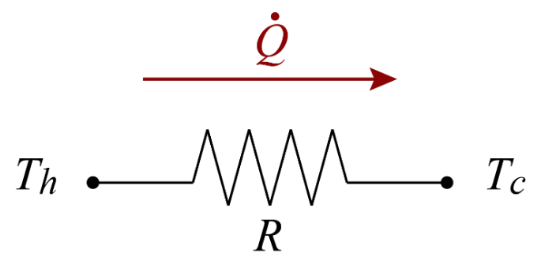
\includegraphics[scale=0.7]{./images/steady-state-heat-conduction-electrical-resistance-analogy.png}
\end{center}

\subsection{Thermal resistance}
\label{sec:org76e3a4d}
Steady-state heat transfer rate can be expressed in terms of temperature difference divided by the thermal resistance.
\[\dot{Q} = \frac{\Delta T}{R}\]

\subsubsection{Plane wall}
\label{sec:orge8e06b2}
\begin{center}
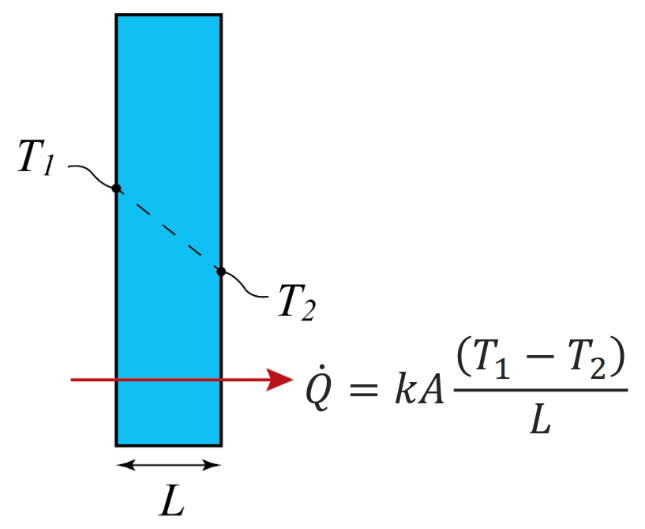
\includegraphics[scale=0.8]{./images/thermal-resistance-plane-wall.png}
\end{center}
\begin{center}
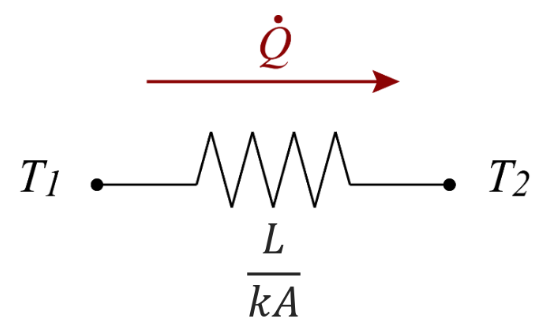
\includegraphics[scale=0.8]{./images/thermal-resistance-plane-wall-electrical-analogy.png}
\end{center}
\begin{itemize}
\item Thermal resistance of a plane wall is given by:
\[R = \frac{L}{kA} \quad \unit{K.W^{-1}}\]
\item The heat transfer rate is given by:
\[\dot{Q} = kA \frac{T_1 - T_2}{L}\]
\end{itemize}

\subsubsection{Cylindrical wall}
\label{sec:org1e5b133}
\begin{center}
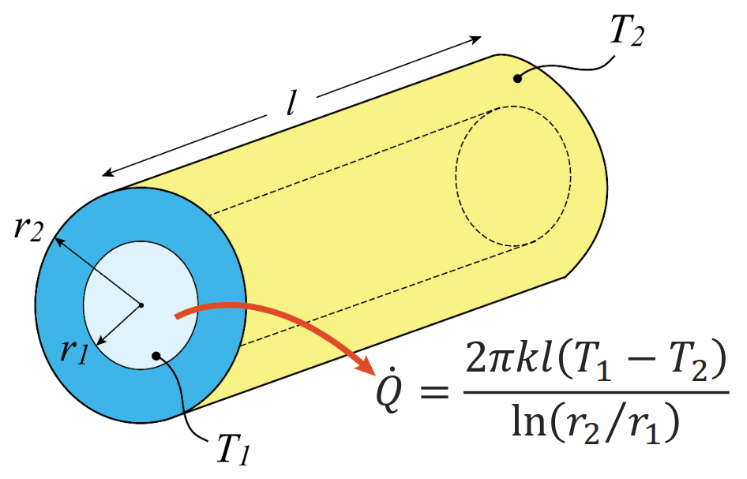
\includegraphics[scale=1]{./images/thermal-resistance-cylindrical-wall.png}
\end{center}
\begin{center}
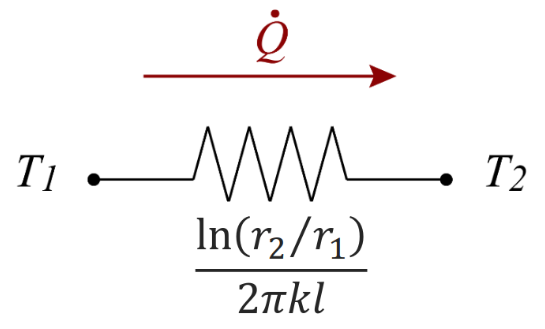
\includegraphics[scale=1]{./images/thermal-resistance-cylindrical-wall-electrical-analogy.png}
\end{center}
\begin{itemize}
\item Thermal resistance of a cylindrical wall is given by:
\[R = \frac{\ln \left(\frac{r_2}{r_1} \right)}{2 \pi k l}\]
\item The heat transfer is in the normal direction to flow, which is through the pipe wall.
\[\dot{Q} = \frac{2 \pi kl (T_1 - T_2)}{\ln \left(\frac{r_2}{r_1} \right)}\]
\end{itemize}

\subsubsection{Spherical wall}
\label{sec:org7f484f6}
\begin{center}
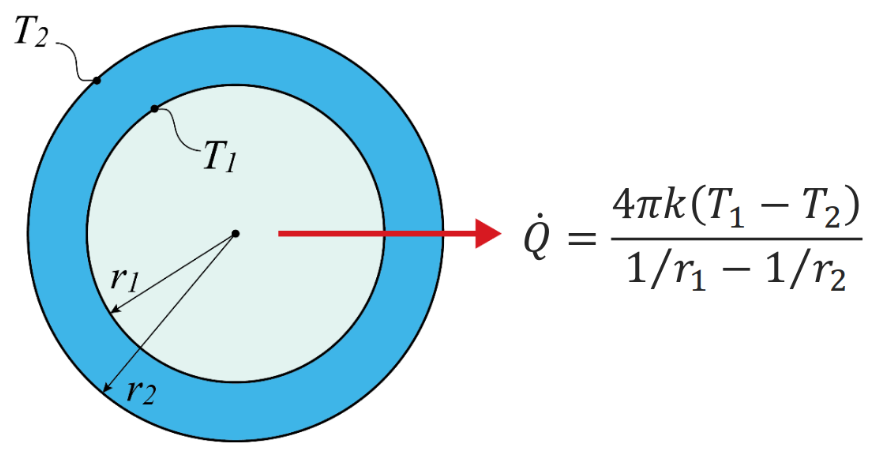
\includegraphics[scale=1]{./images/thermal-resistance-spherical-wall.png}
\end{center}
\begin{center}
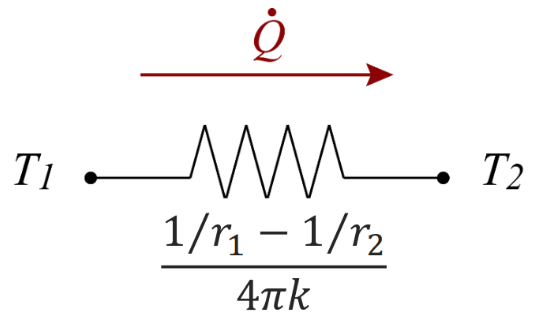
\includegraphics[scale=1]{./images/thermal-resistance-spherical-wall-electrical-analogy.png}
\end{center}
\begin{itemize}
\item Thermal resistance of a spherical wall (radial direction)
\[R = \frac{\frac{1}{r_1} - \frac{1}{r_2}}{4 \pi k}\]
\item The heat transfer rate is given by:
\[\dot{Q} = \frac{4 \pi k (T_1 - T_2)}{\frac{1}{r_1} - \frac{1}{r_2}}\]
\end{itemize}

\subsubsection{Convection}
\label{sec:orge8e0f09}
\begin{center}
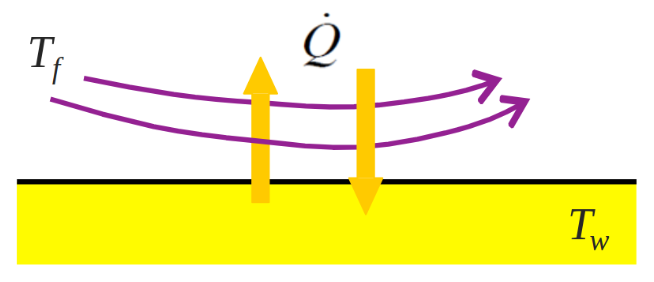
\includegraphics[scale=1]{./images/thermal-resistance-convection.png}
\end{center}
\begin{center}
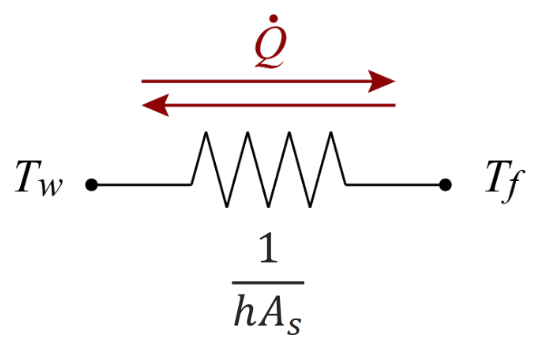
\includegraphics[scale=1]{./images/thermal-resistance-convection-electrical-analogy.png}
\end{center}
\begin{itemize}
\item Steady-state convection heat transfer
\[\dot{Q} = h A_s (T_w - T_f) \quad \textbf{Newton's law of cooling}\]
\item Thermal resistance for convection heat transfer:
\[R = \frac{1}{h A_s}\]
\end{itemize}

 \newpage

\subsubsection{Radiation}
\label{sec:org02e9790}
\begin{center}
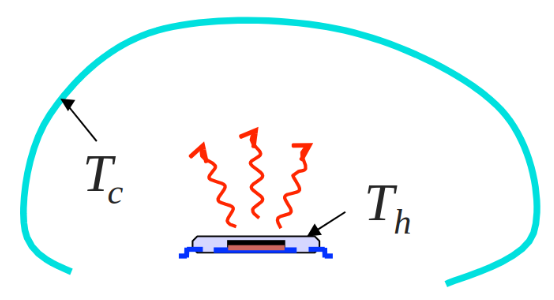
\includegraphics[scale=1]{./images/thermal-resistance-radiation.png}
\end{center}
\begin{center}
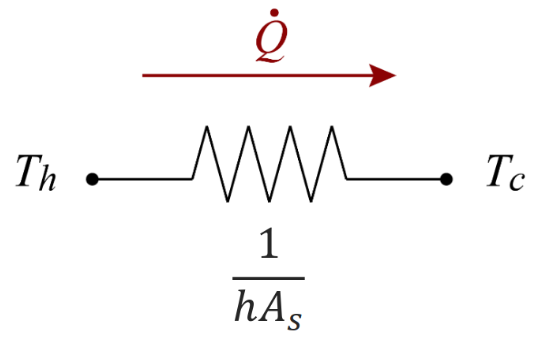
\includegraphics[scale=1]{./images/thermal-resistance-radiation-electrical-analogy.png}
\end{center}
\begin{itemize}
\item Steady-state radiation heat transfer:
\[\dot{Q} = \varepsilon \sigma A_s (T_h^4 - T_c^4) = h_r A_s \Delta T\]

Where \(h_r = \varepsilon \sigma (T_h^2 + T_c^2)(T_h + T_c)\)
\item Thermal resistance for radiation heat transfer:
\[R = \frac{1}{h_r A_s}\]
\end{itemize}

 \newpage

\subsection{Analysis of steady-state heat transfer}
\label{sec:orgad079a7}
\begin{itemize}
\item Consider heat transfer through a plane wall, with convection heat transfer on both sides of the wall:
\begin{center}
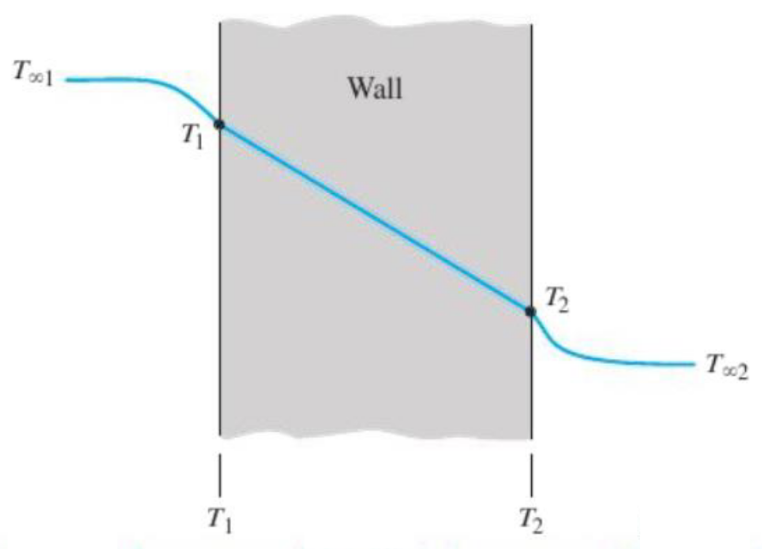
\includegraphics[width=.9\linewidth]{./images/analysis-of-steady-state-heat-transfer.png}
\end{center}
\item For steady-state conditions:
\begin{center}
\begin{tabular}{>{\centering\arraybackslash}m{10em} >{\centering\arraybackslash}m{1em} >{\centering\arraybackslash}m{10em} >{\centering\arraybackslash}m{1em} >{\centering\arraybackslash}m{10em}}
Rate of \textbf{heat convection} into the wall & \(=\) & Rate of \textbf{heat conduction} through the wall & \(=\) & Rate of \textbf{heat convection} from the wall\\[0pt]
\(\dot{Q} = h_1 A (T_{\infty 1})\) & \(=\) & \(kA \frac{T_1 - T_2}{L}\) & \(=\) & \(h_2 A (T_2 - T_{\infty 2})\)\\[0pt]
\end{tabular}
\end{center}
\item Rearranging:
\[\dot{Q} = \frac{(T_{\infty 1} - T_1)}{\frac{1}{h_1 A}} = \frac{T_1 - T_2}{\frac{L}{kA}} = \frac{(T_2 - T_{\infty 2})}{\frac{1}{h_2 A}}\]
\[\dot{Q} = \frac{(T_{\infty 1} - T_1)}{R_{\text{conv, 1}}} = \frac{T_1 - T_2}{R_{wall}} = \frac{(T_2 - T_{\infty 2})}{R_{\text{conv, 2}}}\]
\end{itemize}

 \newpage

\begin{itemize}
\item Individual thermal resistances can be rearranged as shown to model heat transfer through the wall:
\begin{center}
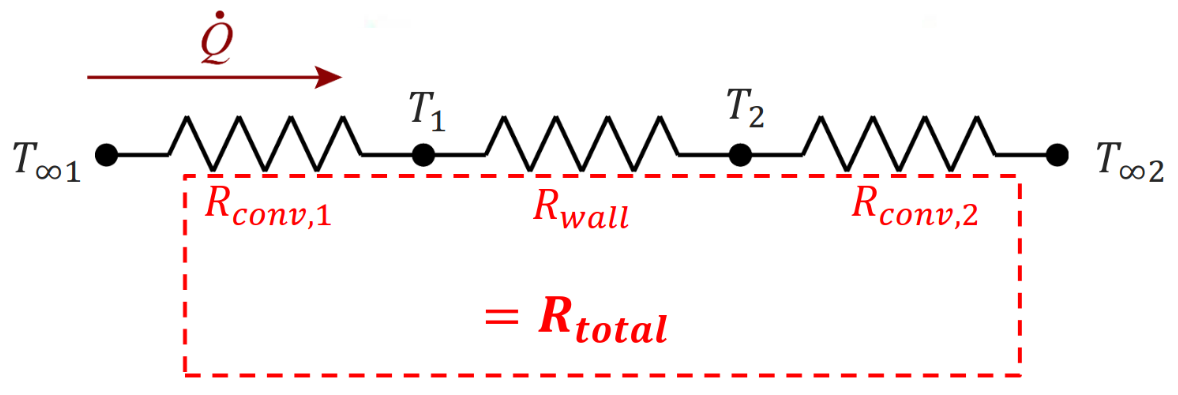
\includegraphics[width=.9\linewidth]{./images/analysis-of-steady-state-heat-transfer-electrical-analogy.png}
\end{center}
\item Heat flow:
\[\dot{Q} = \frac{T_{\infty 1} - T_{\infty 2}}{R_{\text{conv, 1}} + R_{wall} + R_{\text{conv, 2}}} = \frac{T_{\infty 1} - T_{\infty 2}}{R_{total}} \quad (\text{Thermal network})\]
\item If the thermal resistances and temperatures at the end points are known, heat transfer rate can be calculated \textbf{without} evaluation of wall temperatures \(T_1\) and \(T_2\).
\item Heat transfer rate:
\[\dot{Q} = \frac{T_{\infty 1} - T_{\infty 2}}{R_{\text{conv, 1}} + R_{wall} + R_{\text{conv, 2}}} = \frac{T_{\infty 1} - T_{\infty 2}}{R_{total}}\]
\item The above equation can be expressed in a similar form to Newton's law of cooling:
\[\dot{Q} = UA \Delta T\]

Where:
\begin{itemize}
\item \(U\) is the \textbf{overall heat transfer coefficient} in \(\unit{W.m^{2}.K}\)
\item \(UA = \frac{\dot{Q}}{\Delta T} = \frac{1}{R_{total}}\)
\end{itemize}
\end{itemize}

 \newpage

\subsection{Thermal resistance network}
\label{sec:orge66cda1}
For composite walls, evaluation of equivalent thermal resistance follows the same rules and methods used for electrical resistances.

\subsubsection{Resistances in series}
\label{sec:org600dd87}
\begin{center}
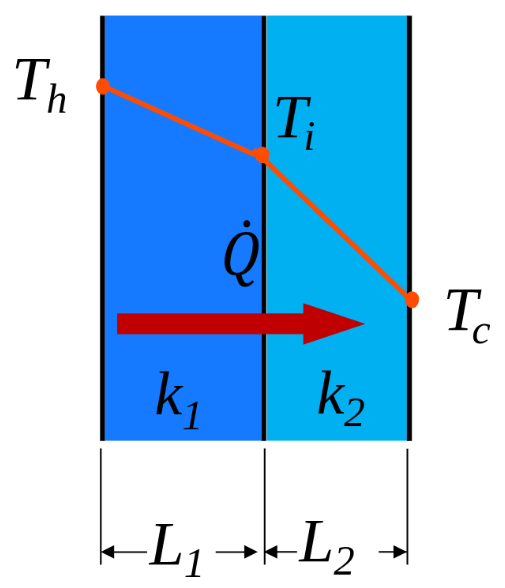
\includegraphics[scale=0.7]{./images/thermal-resistances-in-series.png}
\end{center}
\begin{center}
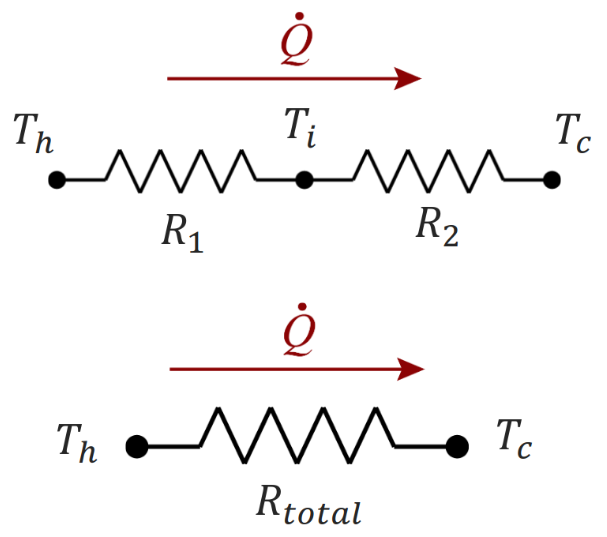
\includegraphics[scale=0.7]{./images/thermal-resistances-in-series-electrical-analogy.png}
\end{center}
\[R_{total} = R_1 + R_2 = \frac{L_1}{k_1 A} + \frac{L_2}{k_2 A}\]
\[\dot{Q} = \frac{T_h - T_c}{R_{total}}\]

\subsubsection{Resistances in parallel}
\label{sec:orgb0985a7}
\begin{center}
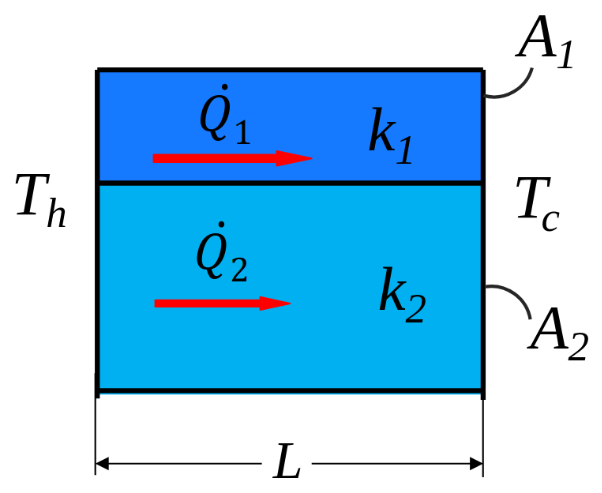
\includegraphics[width=.9\linewidth]{./images/thermal-resistances-in-parallel.png}
\end{center}
\begin{center}
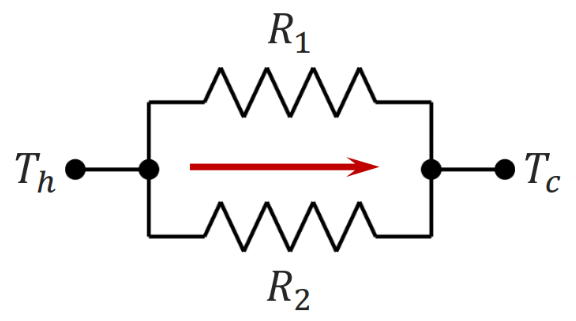
\includegraphics[width=.9\linewidth]{./images/thermal-resistances-in-parallel-electrical-analogy.png}
\end{center}
\[\frac{1}{R_{total}} = \frac{1}{R_1} + \frac{1}{R_2}\]
\[\dot{Q} = \frac{T_h - T_c}{R_{total}}\]

\subsubsection{Combined series-parallel resistances}
\label{sec:orga6af07e}
\begin{center}
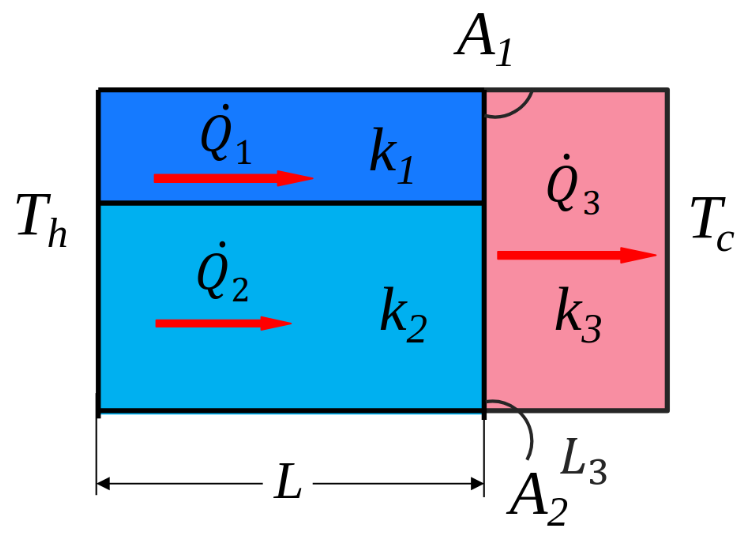
\includegraphics[width=.9\linewidth]{./images/thermal-resistances-combined.png}
\end{center}
\begin{center}
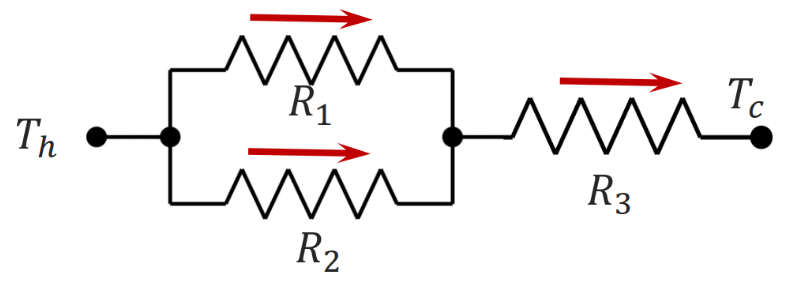
\includegraphics[width=.9\linewidth]{./images/thermal-resistances-combined-electrical-analogy.png}
\end{center}
\[R_1 = \frac{L_1}{k_1 A_1} \quad R_2 = \frac{L_2}{k_2 A_2} \quad R_3 = \frac{L_3}{k_3 A_3}\]
\[R_{total} = R_{1 + 2} + R_3 = \frac{R_1 R_2}{R_1 + R_2} + R_3\]
\[\dot{Q}_3 = \dot{Q}_1 + \dot{Q}_2\]
\[\dot{Q} = \dot{Q}_3 = \frac{T_h - T_c}{R_{total}}\]

\subsubsection{Remarks}
\label{sec:orgb783643}
\begin{itemize}
\item Most heat transfer analysis occur under steady conditions and surface temperature.
\item It is useful for analysing practical steady-state heat transfer problems.
\item No need to solve conduction differential equations.
\begin{itemize}
\item Heat transfer applications reduced to a thermal circuit (thermal resistance network)
\item Thermal circuit can be solved using the same rules and methods used for solving electrical resistance circuits.
\end{itemize}
\item \textbf{Not applicable} for solids experiencing \textbf{internal heat generation}.
\item Outside of solid with heat generation, thermal resistance networks can still apply.
\item There might be \textbf{thermal contact resistances} between solids that are in \textbf{imperfect contact} with each other.
\item Assume no thermal contact resistance when solving problems.
\end{itemize}

 \newpage

\subsection{Thermal contact resistance}
\label{sec:orgb044ee4}
\begin{itemize}
\item Consider a 2-layer composite plane wall with perfect contact at the interface:
\begin{itemize}
\item The heat is conducted across uniformly.
\end{itemize}
\item In reality, there is imperfect contact (surface roughness) resulting in \textbf{non-uniform heat transfer} across the surface.
\begin{itemize}
\item Air gaps act as insulators due to low thermal conductivity of air.
\item Heat transfer by conduction and radiation.
\item Temperature drop across interface.
\end{itemize}
\end{itemize}
\begin{center}
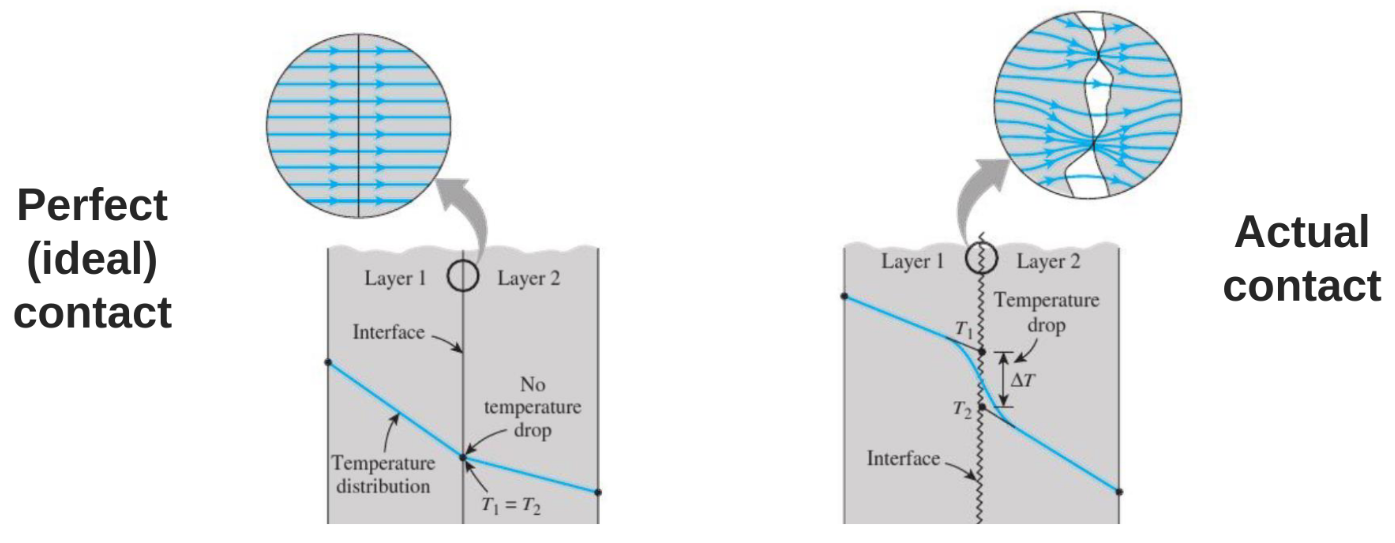
\includegraphics[width=.9\linewidth]{./images/thermal-contact-resistance.png}
\end{center}

\subsection{Transient heat transfer}
\label{sec:org96ed131}
\begin{itemize}
\item Non-steady heat transfer analysis:
\[T = T(x, y, z, t)\]
\item Some bodies are observed to behave like a "lump", in which the \textbf{internal temperature} remains \textbf{uniform} at all times during heat transfer.
\begin{itemize}
\item \textbf{Lumped system analysis} is the simplest model for transient heat transfer.
\item \textbf{Uniform temperature distribution} within the body.
\end{itemize}
\item All small copper ball can be modelled as a lumped system, but a roast beef cannot:
\end{itemize}

\subsection{Characteristic length (\(L_c\)) of a body}
\label{sec:orgca0e547}
\[L_c = \frac{V}{A_s} \quad (\unit{m})\]

Where:
\begin{itemize}
\item \(V\) is the volume of the body
\item \(A_s\) is the exposed surface area of the body
\end{itemize}

 \newpage

\subsection{Lumped system analysis}
\label{sec:orgefb29bb}
\begin{center}
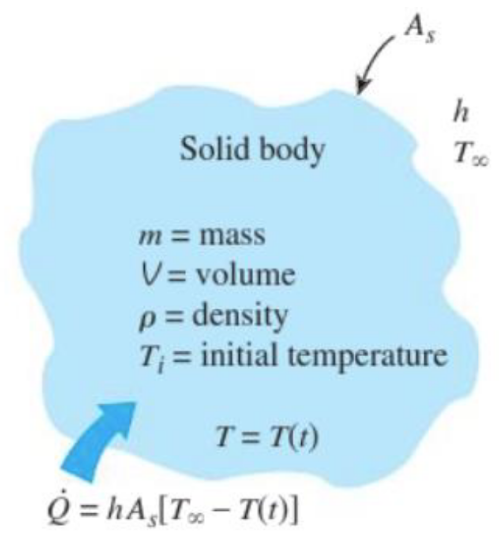
\includegraphics[width=.9\linewidth]{./images/lumped-system-analysis-diagram.png}
\end{center}
\begin{itemize}
\item Recall the heat conduction equation with no heat generation:
\begin{align*}
k \frac{\partial^2 T}{\partial x^2} + \dot{e}_{gen} &= \rho c \frac{\partial T}{\partial t} \\
k \frac{\partial^2 T}{\partial x^2} &= \rho c \frac{\partial T}{\partial t} \\
\rightarrow T(t) &= \text{constant} \quad \because \frac{\partial^2 T}{\partial x^2} = 0 \quad \text{for uniform internal temperature}
\end{align*}

 \newpage

\item For heat transfer into the body during a differential time \(dt\), the temperature of the body rises by a differential amount \(dT\).
\begin{center}
\begin{tabular}{>{\centering\arraybackslash}m{15.5em} >{\centering\arraybackslash}m{1em} >{\centering\arraybackslash}m{17em}}
Heat transfer into a body during \(dt\) & \(=\) & Increase in energy of body during \(dt\)\\[0pt]
\(h A_s (T_{\infty} - T) dt\) & \(=\) & \(mc dT = \rho V c dT\)\\[0pt]
\end{tabular}
\end{center}
\item Since \(T_{\infty}\) is a constant, \(dT = d(T - T_{\infty})\):
\[hA_s (T_{\infty} - T) dt = \rho V c d(T - T_{\infty})\]
\item Rearranging:
\[\frac{d(T - T_{\infty})}{T - T_{\infty}} = - \frac{h A_s}{\rho V c} dt\]
\item Integrating from initial conditions \(T(t = 0) = T_i\):
\[\int_{T_i}^{T = T(t)} \frac{d(T - T_{\infty})}{T - T_{\infty}} = \int_0^t - \frac{h A_s}{\rho V c} dt \quad \rightarrow \quad \ln \frac{T(t) - T_{\infty}}{T_i - T_{\infty}} = - \frac{h A_s}{\rho V c} t\]
\[\frac{T(t) - T_{\infty}}{T_i - T_{\infty}} = e^{-bt} \quad \text{or} \quad t = - \tau \ln \left[\frac{T(t) - T_{\infty}}{T_i - T_{\infty}} \right]\]

Where:
\begin{itemize}
\item \(b = \frac{h A_s}{\rho V c} \ (\unit{s^{-1}})\), to determine the temperature \(T(t)\) of a body at time \(t\)
\item \(\tau\) is the time constant, the reciprocal of \(b\), which is to determine the time \(t\) required for the temperature to reach a specified value \(T(t)\), given by:
\[\tau = \frac{1}{b} = \frac{\rho V c}{h A_s} \quad (\unit{s})\]
\end{itemize}

 \newpage

\item Temperature of the body approaches the ambient temperature exponentially.
\end{itemize}

\begin{center}
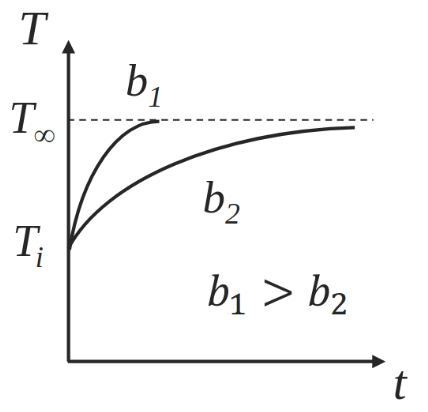
\includegraphics[width=0.49\textwidth]{./images/lumped-system-analysis-temperature-increasing-graph.png}
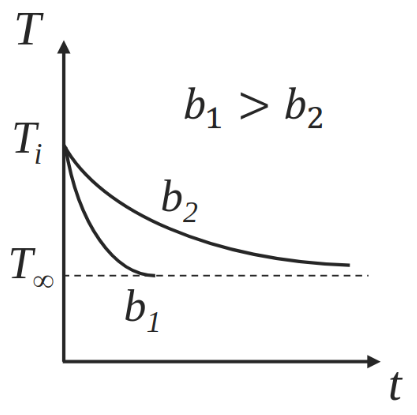
\includegraphics[width=0.49\textwidth]{./images/lumped-system-analysis-temperature-decreasing-graph.png}
\end{center}

\begin{itemize}
\item \textbf{Instantaneous rate} of heat transfer at any time \(t\):
\[\dot{Q}(t) = h A_s [T(t) - T_{\infty}]\]
\item \textbf{Total amount} of heat transferred at time \(t\):
\[Q = mc[T(t) - T_i]\]
\item \textbf{Maximum limit} of heat transfer occurs at equilibrium:
\[Q_{total} = mc[T_{\infty} - T_i]\]

 \newpage

\item Heat transfer stops when body reaches equilibrium temperature with the ambient temperature.
\begin{center}
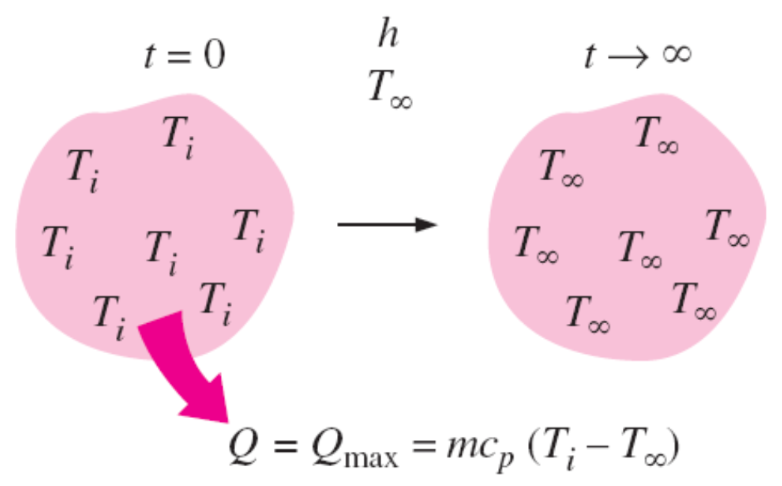
\includegraphics[width=.9\linewidth]{./images/lumped-system-analysis-temperature-reach-ambient-diagram.png}
\end{center}
\[Q = Q_{max} = mc_{p} (T_i - T_{\infty})\]
\end{itemize}

 \newpage

\subsubsection{Criteria}
\label{sec:org4376b0f}
\begin{itemize}
\item Lumped system analysis is only \textbf{valid} when \textbf{temperature distribution} in the body is \textbf{uniform}.
\begin{itemize}
\item Ensure that temperature variation in the body is not drastic in order to use lumped system analysis.
\item Rate of conduction within the body has to be relatively quick.
\end{itemize}
\item For example, if the rate of convection heat transfer is much higher than the rate of conduction within the body:
\begin{itemize}
\item Surface temperature of the body will be different form its internal temperature.
\item Lumped system analysis would \textbf{not be valid}.
\end{itemize}
\item The criteria for checking the validity of using the lumped system analysis requires the \textbf{comparison} of the \textbf{rate of convection} heat transfer to the \textbf{rate of conduction} heat transfer within the body.
\item Convection heat transfer is proportional to the surface area of the body.
\item Conduction heat transfer depends on the area and size (length scale) of the body.
\item Using the characteristic length of a body:
\[b = \frac{h A_s}{\rho V c} = \frac{h}{\rho c L_c} \quad (\unit{s^{-1}})\]
\[\tau = \frac{\rho V c}{h A_s} = \frac{\rho c L_c}{h} \quad (\unit{s})\]
\end{itemize}

 \newpage

\subsection{Biot number (\(Bi\))}
\label{sec:org65cf91e}
\begin{itemize}
\item The Biot number (\(Bi\)) is a dimensionless constant that compares the convection heat transfer \textbf{at the surface of the body} to the conduction heat transfer \textbf{within the body}.
\begin{center}
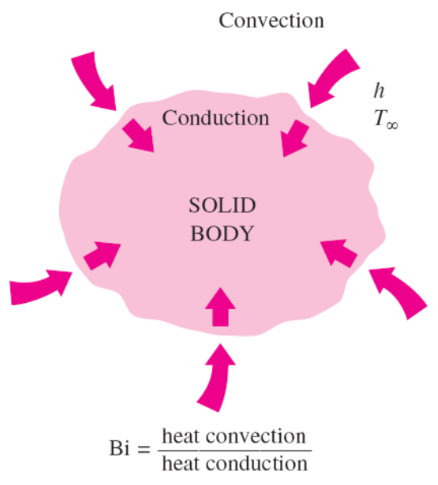
\includegraphics[width=.9\linewidth]{./images/biot-number-diagram.png}
\end{center}
\[Bi = \frac{\text{convection}}{\text{conduction}} = \frac{h}{\frac{k}{L_c}} \frac{\Delta T}{\Delta T}\]
\[Bi = \frac{hL_c}{k}\]
\item Lumped system analysis is only \textbf{valid} when the rate of convection is much slower than the rate of conduction, i.e. Biot number is \textbf{small}:
\[Bi \le 0.1\]
\end{itemize}

\subsubsection{Thermal resistance perspective}
\label{sec:org7dc85d1}
\begin{itemize}
\item The Biot number (\(Bi\)) is also the ratio of \textbf{internal resistance} of a body to heat conduction to its \textbf{external resistance} to heat convection:
\begin{align*}
Bi &= \frac{\text{Convection}}{\text{Conduction}} \\
&= \frac{h}{\frac{k}{L_c}} \frac{\Delta T}{\Delta T} \\
&= \frac{\frac{L_c}{k}}{\frac{1}{h}} \\
&= \frac{\text{Conduction resistance within the body}}{\text{Convection resistance at the surface of the body}}
\end{align*}
\item Lumped system analysis is valid when \(Bi \le 0.1\):
\begin{itemize}
\item Thermal resistance to conduction is very small so that heat can distribute quickly within the body.
\end{itemize}
\end{itemize}

 \newpage

\subsubsection{Diagrams}
\label{sec:org31b5a7d}
\begin{itemize}
\item Small bodies with high thermal conductivities and low convection coefficients are most likely to satisfy the criterion for lumped system analysis.
\begin{center}
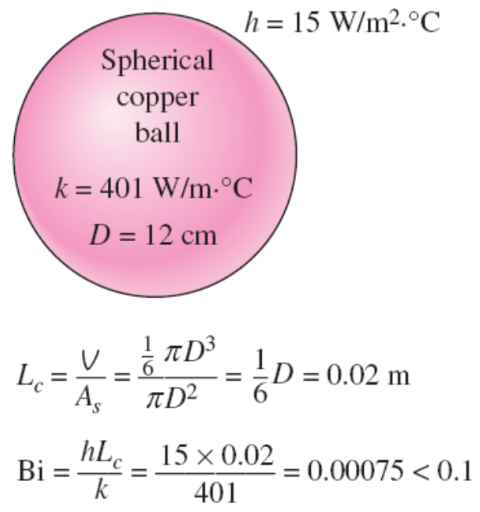
\includegraphics[width=.9\linewidth]{./images/biot-number-spherical-copper-ball.png}
\end{center}
\end{itemize}

 \newpage

\begin{itemize}
\item When the convection coefficient \(h\) is high and \(k\) is low, large temperature differences occur between the inner and outer regions of a large solid.
\begin{center}
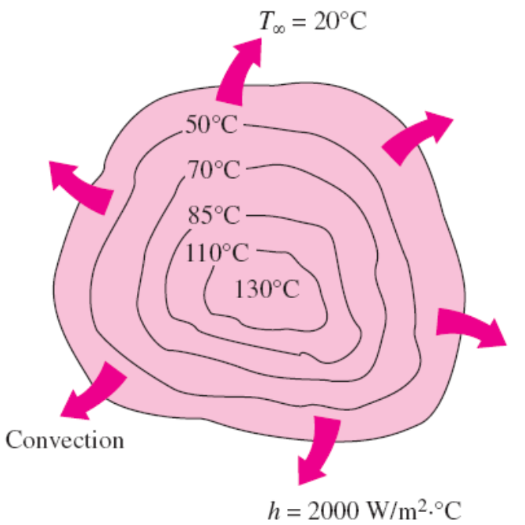
\includegraphics[width=.9\linewidth]{./images/biot-number-large-solid.png}
\end{center}
\end{itemize}

 \newpage

\begin{itemize}
\item Analogy between heat transfer to a solid and passenger traffic to an island.
\begin{center}
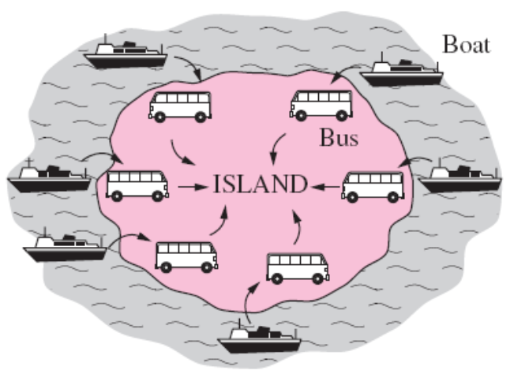
\includegraphics[width=.9\linewidth]{./images/biot-number-island-analogy.png}
\end{center}
\end{itemize}

\subsection{Types of flow in convection}
\label{sec:org365b125}

\subsubsection{Forced flow}
\label{sec:org875e43e}
A fluid is forced to flow over a surface or in a pipe by external means such as a pump or a fan.
\begin{center}
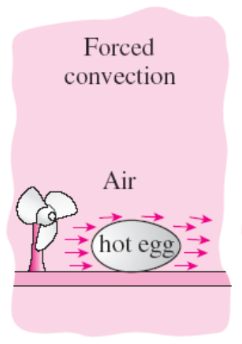
\includegraphics[height=18em]{./images/forced-flow-diagram.png}
\end{center}

\subsubsection{Natural flow}
\label{sec:org0c5096f}
Fluid motion due to natural means such as the buoyancy effect (density). Warmer and lighter fluids rise while cooler and denser fluids fall.
\begin{center}
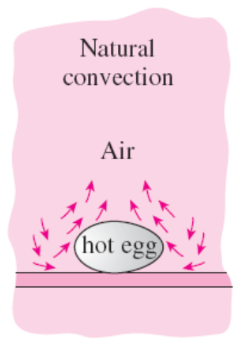
\includegraphics[width=.9\linewidth]{./images/natural-flow-diagram.png}
\end{center}

\subsubsection{External flow}
\label{sec:org5781aa0}
The flow of an unbounded fluid over a surface such as a plate, a wire or a pipe. Some examples include:
\begin{itemize}
\item Flow over a flat plate
\item Flow over cylinder or spheres
\end{itemize}

\begin{center}
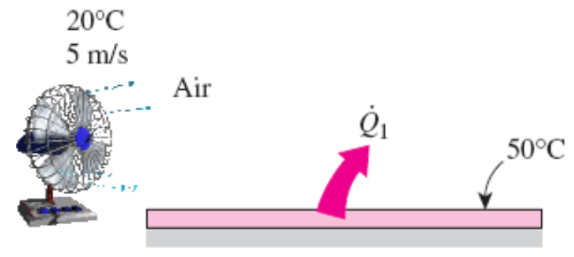
\includegraphics[width=.9\linewidth]{./images/external-flow-diagram.png}
\end{center}

\subsubsection{Internal flow}
\label{sec:org77f1ad1}
The flow in a pipe or duct if the fluid is completely bounded by solid surfaces.
\begin{itemize}
\item Flow between parallel plates
\item Flow inside tubes
\end{itemize}

\begin{center}
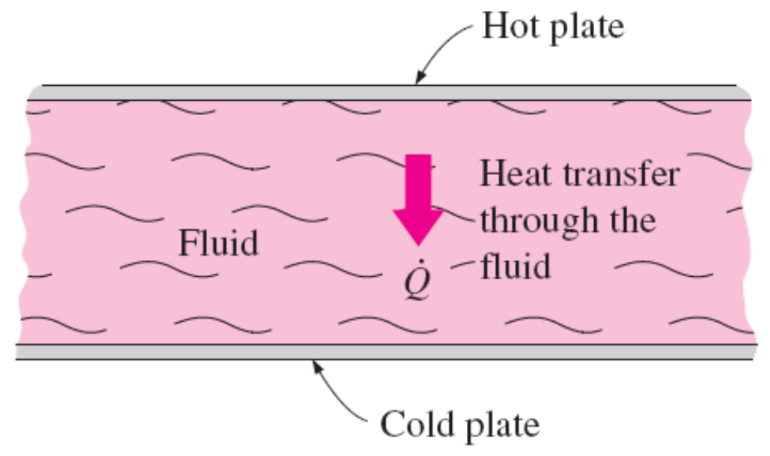
\includegraphics[width=.9\linewidth]{./images/internal-flow-diagram.png}
\end{center}

\subsubsection{Open-channel flow (not tested)}
\label{sec:orge1d93ed}
The flow in a pipe or duct is only partially filled with the liquid and there is a free surface.

\subsubsection{Steady flow}
\label{sec:org9248c04}
\begin{itemize}
\item The term \textbf{steady} implies that there is no change with respect to time.
\item Many devices such as turbines, compressors, boilers, condensers, and heat exchangers operate for long periods of time under the same conditions, and they are classified as \textbf{steady-flow devices}.
\end{itemize}

\subsubsection{Unsteady flow}
\label{sec:org7e9e487}
Unsteady flow means the flow changes with time, which is the opposite of steady flow.

\subsubsection{Uniform flow}
\label{sec:org3888979}
Uniform flow refers to flow that does not change in location over a specified region.

\subsubsection{Periodic flow}
\label{sec:orgba0fa12}
Periodic flow is a kind of \textbf{unsteady} flow in which the flow oscillates about a \textbf{steady mean}.

 \newpage

\subsection{Physical mechanism of convection}
\label{sec:orgfb07b2e}
The fluid motion brings warmer and cooler chunks of fluid into contact, initiating higher rates of conduction at a greater number of sites in a fluid. The rate of heat transfer through a fluid by convection is \textbf{much higher} than by conduction.  \\

Head transfer through a fluid sandwiched between two parallel plates:
\begin{center}
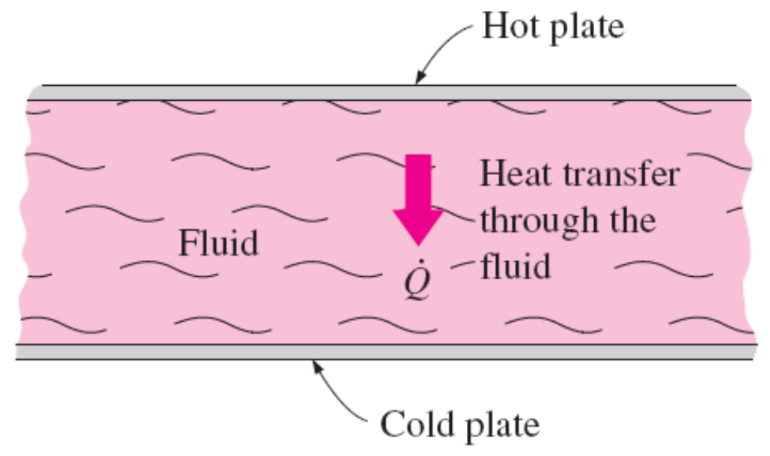
\includegraphics[width=.9\linewidth]{./images/internal-flow-diagram.png}
\end{center}

\subsection{Convection heat transfer coefficient (\(h\))}
\label{sec:orgaeed622}
Convection heat transfer coefficient is the rate of heat transfer between a \textbf{solid surface} and \textbf{a fluid} per unit surface area per unit temperature difference. \(h\) has units \(\unit{W.m^{-2}.K^{-1}}\).

\subsubsection{In forced convection}
\label{sec:org5a2b922}
\(h\) in \textbf{forced convection} depends on:
\begin{enumerate}
\item Fluid properties, which includes dynamic viscosity, thermal conductivity, density, and specific heat.
\item Fluid velocity.
\item Type of fluid flow, either streamlined or laminar, or turbulent.
\item Geometry and the roughness of the solid surface.
\end{enumerate}

\subsection{Convection heat transfer}
\label{sec:org8eb3024}

\subsubsection{Heat transfer rate}
\label{sec:org5be603f}
\[\dot{Q}_{conv} = h A_s (T_s - T_{\infty}) \quad (\unit{W})\]

Where:
\begin{itemize}
\item \(\dot{Q}_{conv}\) is the convection heat transfer rate
\item \(h\) is the convection heat transfer coefficient (\(\unit{W.m^{-2}.K^{-1}}\))
\item \(A_s\) is the heat transfer surface area (\(\unit{m^{2}}\))
\item \(T_s\) is the temperature of the surface (\(\unit{\degreeCelsius}\))
\item \(T_{\infty}\) is the temperature of the fluid sufficiently far from the surface (\(\unit{\degreeCelsius}\))
\end{itemize}

\subsubsection{Heat flux}
\label{sec:org7e1bd89}
\[\dot{q}_{conv} = h (T_s - T_{\infty}) \quad (\unit{W.m^{-2}.K^{-1}})\]

Where:
\begin{itemize}
\item \(\dot{q}_{conv}\) is the convection heat flux
\item \(h\) is the convection heat transfer coefficient (\(\unit{W.m^{-2}.K^{-1}}\))
\item \(T_s\) is the temperature of the surface (\(\unit{\degreeCelsius}\))
\item \(T_{\infty}\) is the temperature of the fluid sufficiently far from the surface (\(\unit{\degreeCelsius}\))
\end{itemize}

 \newpage

\subsection{No-slip boundary condition}
\label{sec:org99b46f1}
An assumption that a fluid in direct contact with a solid "sticks" to the surface due to viscous effects, which results in a non-uniform velocity profile.

\subsubsection{Heat transfer}
\label{sec:org2084872}
\begin{itemize}
\item On the wall surface, a fluid layer sticks to the surface (motionless), hence heat transfer is by \textbf{pure conduction}.
\begin{center}
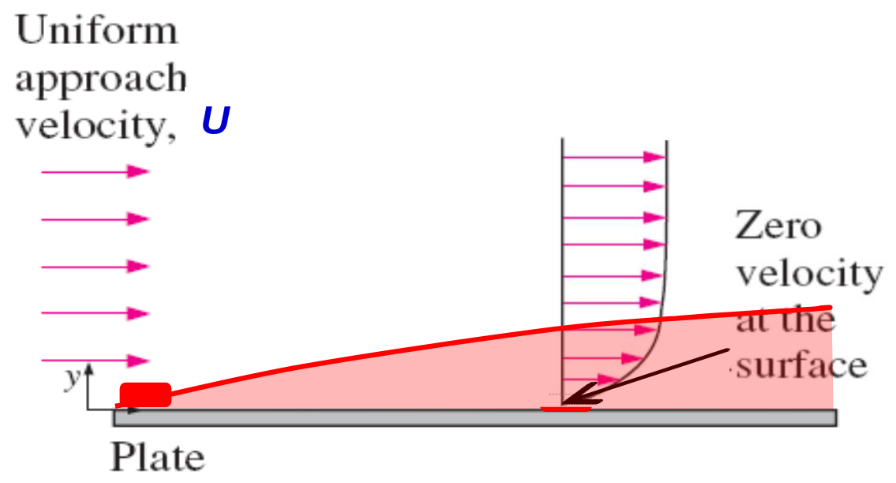
\includegraphics[width=.9\linewidth]{./images/no-slip-boundary-condition-diagram.png}
\end{center}

\[\dot{q}_{conv} = \dot{q}_{cond} = - k_{fluid} \left. \frac{\partial T}{\partial y} \right|_{y = 0} \quad (\unit{W.m^{-2}})\]

\item If the temperature distribution within the fluid is known, \(h\) can be obtained from:
\[h = \frac{-k_{fluid} \left(\frac{\partial T}{\partial y} \right)_{y=0}}{T_s - T_{\infty}} \quad (\unit{W.m^{-2}.\degreeCelsius^{-1}})\]
\end{itemize}

 \newpage

\subsection{Local heat transfer coefficient (\(h_{local}\))}
\label{sec:orgdb3497e}
\(h\) generally varies along the flow (or \(x\)) direction. The \textbf{average} or \textbf{mean} \(h\) for a surface is determined by properly averaging the \textbf{local} \(h\) over the entire surface area \(A_s\), or length \(L\):
\[h = \frac{1}{A_s} \int_{A_s} h_{local} \, dA_s\]
\[h = \frac{1}{L} \int_0^L h_x \, dx\]

\begin{center}
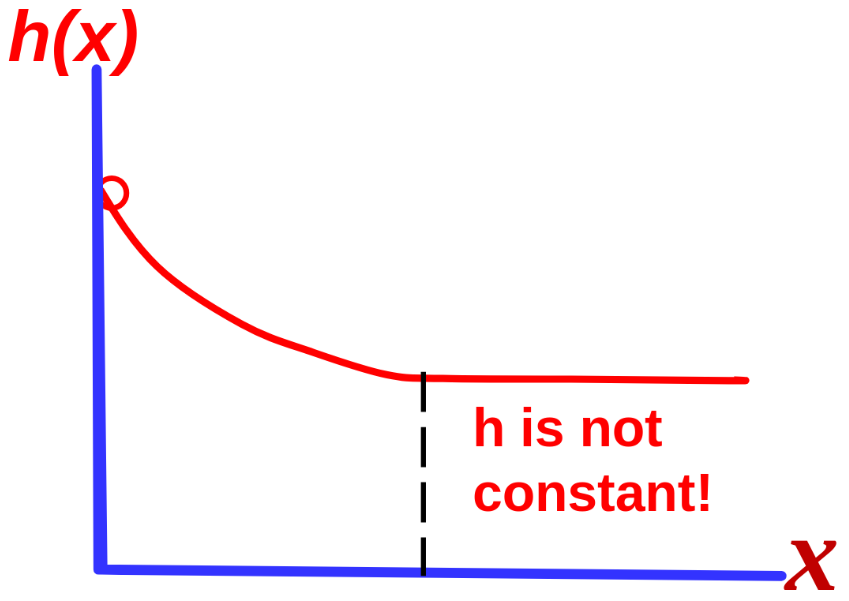
\includegraphics[width=.9\linewidth]{./images/local-heat-transfer-coefficient-graph.png}
\end{center}

 \newpage

\subsection{Thermal boundary layer}
\label{sec:orgeb6677a}
\begin{itemize}
\item Heat transfer from solid surface transfers to the fluid through the thermal boundary layer.
\item The thermal boundary layer is the flow region over the surface in which the \textbf{temperature variation} in the direction \textbf{normal} to the surface is \textbf{significant}.
\item The thickness of the thermal boundary layer (\(\delta_t\)) at any location along the surface is defined as the distance from the surface at which the temperature difference \(T - T_s\) equals \(0.99 (T_{\infty} - T_s)\).
\end{itemize}

\begin{figure}[htbp]
\centering
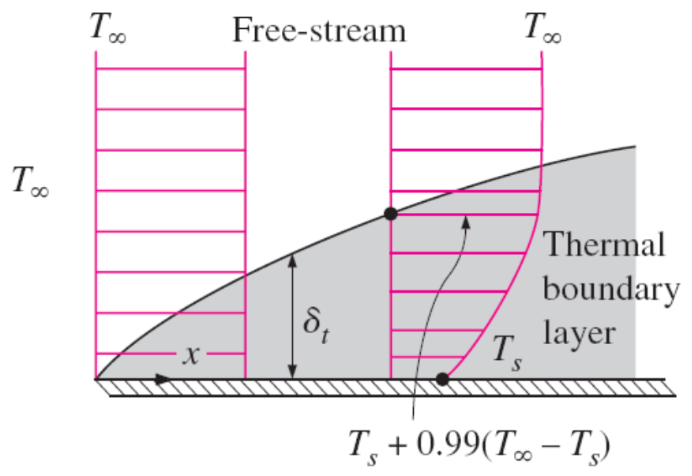
\includegraphics[width=.9\linewidth]{./images/thermal-boundary-layer-diagram.png}
\caption{Thermal boundary layer on a flat plate. The fluid is hotter than the plate surface.}
\end{figure}

 \newpage

\subsection{Temperature profiles}
\label{sec:org95a38fb}
The shape of the temperature profile in the thermal boundary layer dictates the convection heat transfer between a solid surface and the fluid flowing over it.

\subsubsection{\(T_s > T_{\infty}\)}
\label{sec:orgc67fb2d}
\begin{center}
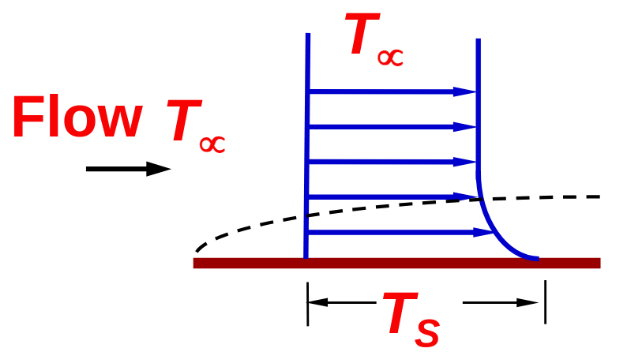
\includegraphics[width=.9\linewidth]{./images/temperature-profile-ts-greater-than-t-infinity.png}
\end{center}

\subsubsection{\(T_s < T_{\infty}\)}
\label{sec:org1e47160}
\begin{center}
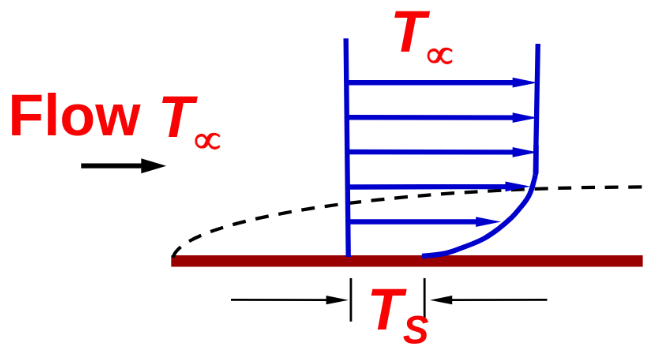
\includegraphics[width=.9\linewidth]{./images/temperature-profile-ts-less-than-t-infinity.png}
\end{center}

\subsubsection{Isothermal flow (\(T_s = T_{\infty}\))}
\label{sec:org239b211}
\begin{center}
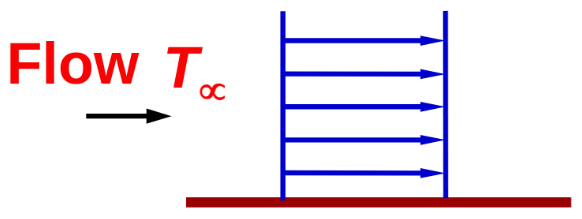
\includegraphics[width=.9\linewidth]{./images/temperature-profile-isothermal-flow.png}
\end{center}

\subsection{Velocity boundary layer}
\label{sec:org319431c}
\begin{itemize}
\item The velocity boundary layer is the region of the flow above the plate bounded by \(\delta\) in which the effects of the viscous shearing forces caused by fluid viscosity are felt.
\item The \textbf{boundary layer thickness}, \(\delta\), is typically defined as the distance \(y\) from the surface at which \(u = 0.99V\), where \(V\) is the free stream velocity of the uniform approach velocity.
\item The hypothetical line of \(u = 0.99V\) divides the flow over a plate into two regions:
\begin{center}
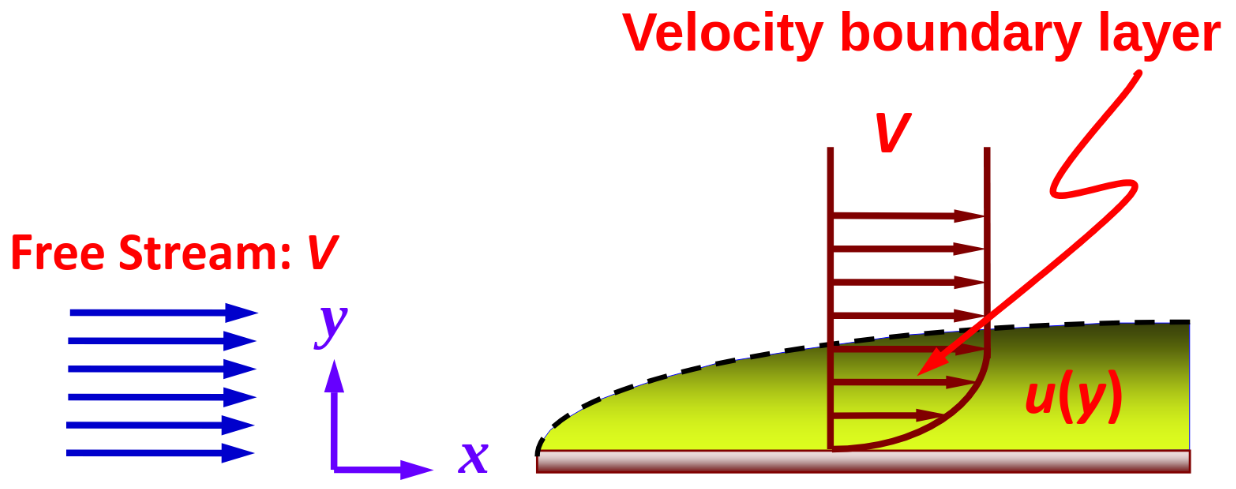
\includegraphics[width=.9\linewidth]{./images/velocity-boundary-layer-diagram.png}
\end{center}
\end{itemize}

\subsubsection{Flow regions}
\label{sec:org6701004}
\begin{center}
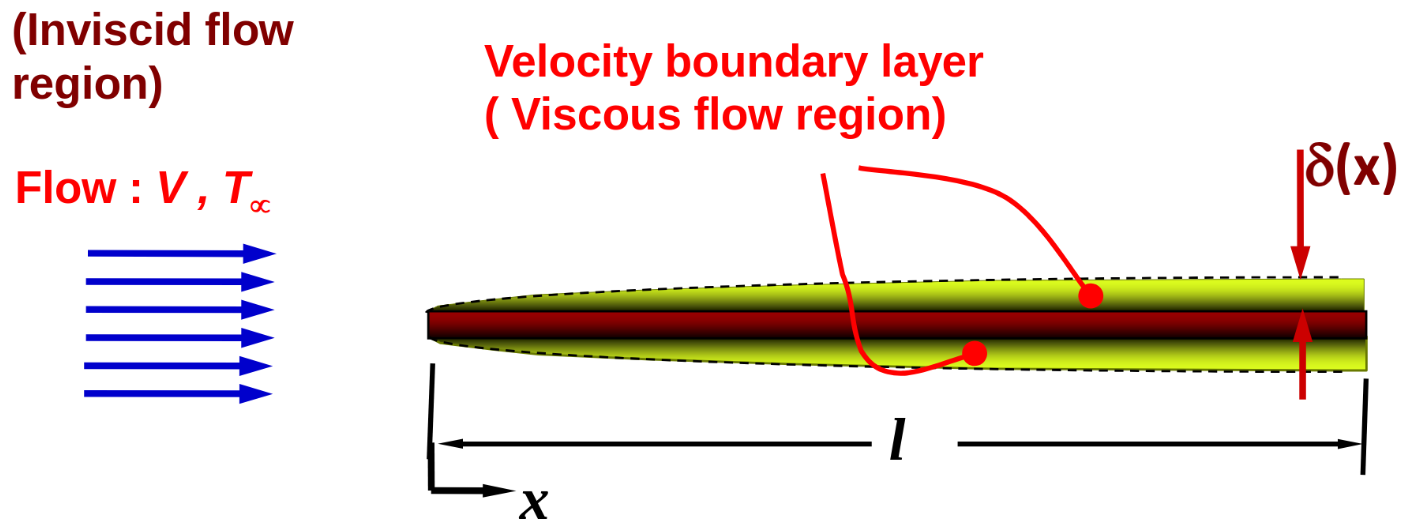
\includegraphics[width=.9\linewidth]{./images/velocity-boundary-layer-flow-regions-diagram.png}
\end{center}
\begin{itemize}
\item Viscous flow region
The viscous effects and the velocity changes are significant in this region.

\item Irrotational flow (inviscid flow) region:
The viscous effects are negligible compared to inertial or pressure forces in this region, and the velocity remains essentially constant. These regions are usually regions that are not close to solid surfaces.
\end{itemize}

\subsection{Thermal vs velocity boundary layer}
\label{sec:org9106869}

\subsubsection{Thermal boundary layer}
\label{sec:org9682191}
\begin{center}
\includegraphics[width=.9\linewidth]{./images/thermal-boundary-layer-all-three-flows.png}
\end{center}

\subsubsection{Velocity boundary layer}
\label{sec:orgadfb7dc}
\begin{center}
\includegraphics[height=10em]{./images/velocity-boundary-layer-simplified-diagram.png}
\end{center}

\subsection{Fluid viscosity (\(\mu\))}
\label{sec:org3e6f5bc}
\begin{itemize}
\item Fluid viscosity is a measure of the internal stickiness of the fluid.
\item It is responsible for the \textbf{no-slip condition} and the development of the boundary layer.
\end{itemize}

\subsubsection{Dynamic viscosity (\(\mu\))}
\label{sec:org7d62578}
Dynamic viscosity is just the fluid's viscosity. It is in \(\unit{kg.m^{-1}.s^{-1}}\) or \(\unit{N.s.m^{-2}}\) or \(\unit{Pa.s}\)

\subsubsection{Kinematic viscosity (\(\nu\))}
\label{sec:org7017eb9}
\[\nu = \frac{\mu}{\rho}\]

Where:
\begin{itemize}
\item \(\nu\) is the kinematic viscosity in \(\unit{m^2.s^{-1}}\) or \textbf{stoke}, where \(\qty{1}{stoke} = \qty{1}{cm^2.s^{-1}} = \qty{0.0001}{m^2.s^{-1}}\)
\item \(\mu\) is the fluid's dynamic viscosity
\item \(\rho\) is the fluid's density
\end{itemize}

\subsection{Friction coefficient (\(C_f\))}
\label{sec:org6cb16b2}
\begin{itemize}
\item The friction coefficient (\(C_f\)) is directly related to the heat transfer coefficient and the power requirements of the pump or fan.
\item Friction coefficient \textbf{varies} with distance along the surface.
\item Friction force over the entire surface:
\[F_f = C_f A_s \frac{\rho V^2}{2} \quad (\unit{N})\]
\end{itemize}

\subsection{Shear stress (\(\tau\))}
\label{sec:org64f622e}
Shear stress if the friction force per unit area. The shear stress for most fluids is proportional to the \textbf{velocity gradient}. For \textbf{Newtonian Fluids}, the shear stress at the \textbf{wall surface} is expressed as:
\[\tau_{w} = \mu \left. \frac{\partial u}{\partial y} \right|_{y=0} \quad (\unit{N.m^{-2}})\]

\subsubsection{Wall shear stress (\(\tau_{w}\))}
\label{sec:org06af424}
During flow, the fluid layer next to the surface will drag the plate along via friction (\textbf{surface drag}). The average wall shear stress is given by
\[\tau_{w} = C_f \frac{\rho V^2}{2} \quad (\unit{N.m^{-2}})\]

\subsection{1, 2 and 3-dimensional flows}
\label{sec:org9bf71a9}
\begin{itemize}
\item A flow field is best characterised by its velocity distribution.
\item A flow is said to be 1, 2, or 3-dimensional if the flow velocity varies in 1, 2 or 3 dimensions, respectively.
\item However, the variation of velocity in certain directions can be small relative to the variation in other directions and can be ignored.

\begin{center}
\includegraphics[width=.9\linewidth]{./images/one-two-and-three-dimensional-flows.png}
\end{center}
\end{itemize}

\subsection{Laminar flow and turbulent flow}
\label{sec:org637c4b0}
\begin{center}
\includegraphics[height=30em]{./images/laminar-and-turbulent-flow-candle-diagram.png}
\includegraphics[width=0.61\textwidth]{./images/laminar-and-turbulent-flow-candle-photo.png}
\end{center}

 \newpage

\subsubsection{Laminar flow}
\label{sec:org360d684}
\begin{itemize}
\item Laminar flow has highly ordered fluid motion (smooth layers of fluid).
\begin{center}
\includegraphics[width=.9\linewidth]{./images/laminar-flow-photo.png}
\end{center}
\item Velocity profile of laminar flow:
\begin{center}
\includegraphics[width=.9\linewidth]{./images/laminar-flow-graph.png}
\end{center}
\end{itemize}

 \newpage

\subsubsection{Turbulent flow}
\label{sec:orgccd704e}
\begin{itemize}
\item Turbulent flow is highly disordered fluid motion that typically occurs at high velocities.
\begin{center}
\includegraphics[width=.9\linewidth]{./images/turbulent-flow-photo.png}
\end{center}
\item Velocity profile in turbulent flow is much \textbf{fuller} than laminar flow.
\item Intense fluid mixing in turbulent flow as a result of rapid fluctuation (eddies) \textbf{enhances mass, heat and momentum transfer} between fluid particles compared to molecular diffusion in laminar flow.
\item Eddies motion decreases rapidly near the wall due to the no-slip boundary condition, which results in \textbf{large velocity and temperature gradients}.
\item Velocity profile of turbulent flow:
\begin{center}
\includegraphics[height=21em]{./images/turbulent-flow-graph.png}
\end{center}
\end{itemize}

\subsubsection{Transitional flow (not tested)}
\label{sec:org942ee12}
Transitional flow is a flow that alternates between being laminar and turbulent.
\begin{center}
\includegraphics[width=.9\linewidth]{./images/transitional-flow-photo.png}
\end{center}

\subsection{Reynolds number (\(Re\))}
\label{sec:orgb9e1ef7}
\begin{itemize}
\item The transition from laminar to turbulent flow depends on the \textbf{geometry, surface roughness, flow velocity, surface temperature, and type of fluid}.
\item The flow regime depends mainly on the ratio of \textbf{inertial forces} to \textbf{viscous forces}, which is the Reynolds number.
\[Re = \frac{\text{Inertial forces}}{\text{Viscous forces}} = \frac{V_{avg} L_c}{\nu} = \frac{\rho V_{avg} L_c}{\mu}\]
\end{itemize}

\begin{center}
\includegraphics[width=.9\linewidth]{./images/reynolds-number-diagram.png}
\end{center}

\subsubsection{Critical Reynolds number (\(Re_{cr}\))}
\label{sec:orga47b0ce}
The Reynolds number at which the flow becomes turbulent.
\begin{itemize}
\item For external flow over a flat plate, the flow is laminar when \(Re < 5 \times 10^5\)
\item Flow is turbulent at \(5 \times 10^5 \le Re \le 10^7\)
\item For internal flow in pipes, flow is laminar when \(Re < 2300\)
\item Flow is fully turbulent at \(Re > 10,000\)
\end{itemize}

\subsubsection{Large Reynolds numbers}
\label{sec:org6126d6c}
The inertial forces are large relative to the viscous forces, and thus the viscous forces cannot prevent the random and rapid fluctuations of the fluid (\textbf{turbulent}).

\subsubsection{Small or moderate Reynolds numbers}
\label{sec:org6c7fb6a}
The viscous forces are large enough to suppress these fluctuations and to keep the fluid "in line" (\textbf{laminar}).

\subsubsection{At distance \(x\) from leading edge of a flat plate}
\label{sec:org32ee814}
\[Re_x = \frac{\rho V x}{\mu} = \frac{Vx}{\nu}\]

Where:
\begin{itemize}
\item \(Re_{x}\) is the Reynolds number at distance \(x\) from the leading edge of the flat plate
\item \(\rho\) is the density of the fluid
\item \(V\) is the approach velocity of the fluid
\item \(x\) is the distance from the leading edge of the flat plate
\item \(\mu\) is the dynamic viscosity
\item \(\nu\) is the kinematic viscosity
\end{itemize}

\subsubsection{At critical distance \(x_{cr}\) from the leading edge of a flat plate}
\label{sec:org613526d}
\[Re_{cr} = \frac{\rho V x_{cr}}{\mu} = \frac{V x_{cr}}{\nu} = 5 \times 10^5\]

Where:
\begin{itemize}
\item \(Re_{cr}\) is the Reynolds number at critical distance \(x_{cr}\) from the leading edge of the flat plate
\item \(\rho\) is the density of the fluid
\item \(V\) is the approach velocity of the fluid
\item \(x_{cr}\) is the critical distance from the leading edge of the flat plate
\item \(\mu\) is the dynamic viscosity
\item \(\nu\) is the kinematic viscosity
\end{itemize}

\subsection{Thermal diffusivity (\(\alpha\))}
\label{sec:org16962bb}
\[\alpha = \frac{k}{\rho c_p}\]

Where:
\begin{itemize}
\item \(\alpha\) is the thermal diffusivity of the fluid
\item \(k\) is the thermal conductivity of the fluid
\item \(\rho\) is the density of the fluid
\item \(c_p\) is the specific heat capacity at constant pressure of the fluid
\end{itemize}

\subsection{Prandtl number (\(Pr\))}
\label{sec:org60bed78}
\begin{itemize}
\item The relative thickness of the velocity and the thermal boundary layers is best described by the \textbf{dimensionless} parameter \textbf{Prandtl number}.
\[Pr = \frac{\text{Molecular diffusivity of momentum}}{\text{Molecular diffusitivity of heat}} = \frac{\nu}{\alpha} = \frac{\mu c_p}{k}\]

\item The Prandtl numbers of gases are about 1, which indicates that both momentum and heat dissipate through the fluid at about the same rate.
\item Heat diffuses very quickly in liquid metals (\(Pr \ll 1\)) and very slowly in oils (\(Pr \gg 1\)) relative to momentum.
\end{itemize}

 \newpage

\subsection{Nusselt number (\(Nu\))}
\label{sec:org9cd266d}
\begin{itemize}
\item Consider heat transfer through a fluid layer of thickness \(L\) and temperature difference \(\Delta T\).
\[\dot{q}_{conv} = h \Delta T\]
\[\dot{q}_{cond} = k \frac{\Delta T}{L}\]
\[\frac{\dot{q}_{conv}}{\dot{q}_{cond}} = \frac{h \Delta T}{\frac{k \Delta T}{L}} = \frac{hL}{k} = Nu\]

\[Nu = \frac{hL_c}{k}\]

Where:
\begin{itemize}
\item \(k\) is the thermal conductivity of the fluid
\item \(L_c\) is the characteristic length
\end{itemize}
\item The Nusselt number represents the \textbf{enhancement of heat transfer} through a fluid layer as a result of convection relative to conduction across the same fluid layer.
\item The larger the Nusselt number, the more effective the convection.
\[Nu = f(Re, Pr)\]
\end{itemize}

\subsection{Forced convection over a flat plate (all given in the exam)}
\label{sec:orgfa648d1}

\subsubsection{Continuity equation}
\label{sec:org62cf420}
\[\frac{\partial u}{\partial x} + \frac{\partial v}{\partial y} = 0\]

Where:
\begin{itemize}
\item \(\frac{\partial u}{\partial x}\) is the rate of change of velocity of the fluid in the \(x\)-direction with respect to \(x\)
\item \(\frac{\partial v}{\partial y}\) is the rate of change of velocity of the fluid in the \(y\)-direction with respect to \(y\)
\end{itemize}

\subsubsection{Momentum equation}
\label{sec:orgc46960b}
\[u \frac{\partial u}{\partial x} + v \frac{\partial u}{\partial y} = \nu \frac{\partial^2 u}{\partial y^2}\]

Where:
\begin{itemize}
\item \(u\) is the velocity of the fluid in the \(x\)-direction
\item \(v\) is the velocity of the fluid in the \(y\)-direction
\item \(\nu\) is the kinematic viscosity of the fluid
\end{itemize}

\subsubsection{Energy equation}
\label{sec:org8c1591b}
\[u \frac{\partial T}{\partial x} + v \frac{\partial T}{\partial y} = \alpha \frac{\partial^2 u}{\partial y^2}\]

Where:
\begin{itemize}
\item \(u\) is the velocity of the fluid in the \(x\)-direction
\item \(v\) is the velocity of the fluid in the \(y\)-direction
\item \(\alpha\) is the thermal diffusivity of the fluid
\end{itemize}

\subsection{Upstream velocity (\(V\)) [Approach velocity]}
\label{sec:org78ea12d}
Upstream velocity is the velocity of the approaching fluid far ahead of the body.

\subsection{Free-stream velocity (\(V_{\infty}\))}
\label{sec:org860c0fe}
Free-stream velocity is the velocity of the fluid relative to an immersed solid body sufficient far from the body.

 \newpage

\subsection{Convective drag force coefficient (\(C_D\))}
\label{sec:org74a97f9}
\[C_D = \frac{F_D}{\frac{1}{2} \rho V^2 A}\]

Where:
\begin{itemize}
\item \(C_D\) is the convective drag force coefficient
\item \(F_D\) is the drag force
\item \(\rho\) is the density of the fluid
\item \(V\) is the upstream velocity
\item \(A\) is the surface area the heat is transferred through
\end{itemize}

\subsection{Parallel flow over flat plates}
\label{sec:orgdfaffab}
\begin{itemize}
\item Factors that affect the transition of flow from laminar to turbulent, which are all characterised by the Reynolds number:
\begin{itemize}
\item Surface geometry
\item Surface roughness
\item Surface temperature
\item Upstream velocity
\item Type of fluid
\end{itemize}
\end{itemize}

\subsection{External forced convection with laminar flow over flat plates (equations given)}
\label{sec:org57ac774}
Laminar flow occurs when \(Re_x < 5 \times 10^5\).

\subsubsection{Velocity boundary layer thickness (\(\delta\))}
\label{sec:orgf9380e6}
\[\delta = \frac{4.91 x}{\sqrt{Re_x}}\]
\[\delta \propto x^{0.5}\]

Where:
\begin{itemize}
\item \(\delta\) is the velocity boundary layer thickness
\item \(x\) is the distance from the leading edge of the flat plate
\item \(Re_x\) is the Reynolds number
\end{itemize}

\subsubsection{Thermal boundary layer thickness (\(\delta_t\))}
\label{sec:org1efa4c4}
\[\delta_t = \frac{\delta}{Pr^{\frac{1}{2}}} = \frac{4.91x}{Pr^{\frac{1}{3}} \sqrt{Re_x}}\]
\[\delta_t \propto x^{0.5}\]

Where:
\begin{itemize}
\item \(\delta_x\) is the thermal boundary layer thickness
\item \(x\) is the distance from the leading edge of the flat plate
\item \(Re_x\) is the Reynolds number
\item \(Pr\) is the Prandtl number
\end{itemize}

\subsubsection{Local friction coefficient (\(C_{\text{f, x}}\))}
\label{sec:org1138a94}
\[C_{\text{f, x}} = \frac{0.664}{\sqrt{Re_x}}\]
\[C_{\text{f, x}} \propto x^{-0.5}\]

Where:
\begin{itemize}
\item \(C_{\text{f, x}}\) is the local friction coefficient
\item \(x\) is the distance from the leading edge of the flat plate
\item \(Re_x\) is the Reynolds number
\end{itemize}

\subsubsection{Local Nusselt number}
\label{sec:orgfd31455}
\[Nu_x = \frac{h_x x}{k} = 0.332 Pr^{\frac{1}{3}} Re_x^{\frac{1}{2}}, Pr \ge 0.6\]
\[h_x \propto x^{-0.5}\]

Where:
\begin{itemize}
\item \(Nu_x\) is the local Nusselt number
\item \(h_x\) is the convective heat transfer coefficient
\item \(k\) is the thermal conductivity of the fluid
\item \(x\) is the distance from the leading edge of the flat plate
\item \(Re_x\) is the Reynolds number
\end{itemize}

\subsubsection{Average friction coefficient (\(C_f\))}
\label{sec:orgf47f443}
\[C_f = \frac{1.328}{\sqrt{Re_L}}\]

Where:
\begin{itemize}
\item \(C_f\) is the average friction coefficient
\item \(Re_L\) is the Reynolds number over the length of the plate
\end{itemize}

\subsubsection{Average Nusselt number (\(\overline{Nu}_L\))}
\label{sec:org8dead33}
\[\overline{Nu}_L = \frac{\bar{h}_L L}{k} = 0.664 Re_L^{\frac{1}{2}} Pr^{\frac{1}{3}}\]

Where:
\begin{itemize}
\item \(\overline{Nu}_L\) is the average Nusselt number
\item \(\bar{h}_L\) is the average heat transfer coefficient over the length of the plate
\item \(L\) is the length of the plate
\item \(k\) is the thermal conductivity of the plate
\item \(Re_L\) is the Reynolds number over the length of the plate
\item \(Pr\) is the Prandtl number
\end{itemize}

\subsection{External forced convection with turbulent flow over flat plates (equations given)}
\label{sec:org9849982}
\begin{itemize}
\item Turbulent flow is when \(5 \times 10^5 \le Re_x \le 10^7\).
\item Turbulent flow has better heat transfer than laminar flow, so it may be beneficial to induce turbulent flow over the entire plate.
\item This is accomplished by adding a turbulence promoter at the leading edge such that the entire flow is turbulent. Some examples include:
\begin{itemize}
\item Fine wire
\item Partial obstruction
\end{itemize}
\item The equations below are valid for:
\begin{itemize}
\item Assuming fully turbulent flow over the entire plate.
\item When the laminar flow region is much smaller than the turbulent region.
\end{itemize}
\end{itemize}

\subsubsection{Velocity boundary layer thickness (\(\delta\))}
\label{sec:orga8ac616}
\[\delta = \frac{0.38 x}{Re_x^{\frac{1}{5}}}\]
\[\delta \propto x^{0.8}\]

Where:
\begin{itemize}
\item \(\delta\) is the velocity boundary layer thickness
\item \(x\) is the distance from the leading edge of the flat plate
\item \(Re_x\) is the Reynolds number
\end{itemize}

\subsubsection{Local friction coefficient (\(C_{\text{f, x}}\))}
\label{sec:orge2ab246}
The local friction and heat transfer rate is higher in turbulent flow because of the intense mixing.
\[C_{\text{f, x}} = \frac{0.059}{Re_x^{\frac{1}{5}}}\]
\[C_{\text{f, x}} \propto x^{-0.2}\]

Where:
\begin{itemize}
\item \(C_{\text{f, x}}\) is the local friction coefficient
\item \(x\) is the distance from the leading edge of the flat plate
\item \(Re_x\) is the Reynolds number
\end{itemize}

\subsubsection{Local Nusselt number}
\label{sec:org746025c}
\[Nu_x = \frac{h_x x}{k} = 0.0296 Pr^{\frac{1}{3}} Re_x^{\frac{4}{5}}, 0.6 \le Pr \le 60\]
\[h_x \propto x^{-0.2}\]

Where:
\begin{itemize}
\item \(Nu_x\) is the local Nusselt number
\item \(h_x\) is the convective heat transfer coefficient
\item \(k\) is the thermal conductivity of the fluid
\item \(x\) is the distance from the leading edge of the flat plate
\item \(Re_x\) is the Reynolds number
\end{itemize}

\subsubsection{Average friction coefficient (\(C_f\))}
\label{sec:orgd6270a8}
\[C_f = \frac{0.074}{Re_L^{\frac{1}{5}}}\]

Where:
\begin{itemize}
\item \(C_f\) is the average friction coefficient
\item \(Re_L\) is the Reynolds number over the length of the plate
\end{itemize}

\subsubsection{Average Nusselt number (\(\overline{Nu}_L\))}
\label{sec:org7d57030}
\[\overline{Nu}_L = \frac{\bar{h}_L L}{k} = 0.037 Re_L^{\frac{4}{5}} Pr^{\frac{1}{3}}\]

Where:
\begin{itemize}
\item \(\overline{Nu}_L\) is the average Nusselt number
\item \(\bar{h}_L\) is the average heat transfer coefficient over the length of the plate
\item \(L\) is the length of the plate
\item \(k\) is the thermal conductivity of the plate
\item \(Re_L\) is the Reynolds number over the length of the plate
\item \(Pr\) is the Prandtl number
\end{itemize}

\subsubsection{Friction coefficient for rough surfaces (\(C_f\))}
\label{sec:orged0cf54}
\[C_f = \left(1.89 - 1.62 \log \frac{\varepsilon}{L} \right)^{-2.5}\]

Where:
\begin{itemize}
\item \(C_f\) is the friction coefficient for rough surfaces
\item \(\varepsilon\) is the surface roughness
\item \(L\) is the length of the plate in the flow direction
\end{itemize}

\subsection{External forced convection with mixed flow over flat plates (equations given)}
\label{sec:org73ccff6}
\begin{center}
\includegraphics[width=.9\linewidth]{./images/external-forced-convection-with-mixed-flow-over-flat-plate.png}
\end{center}
\begin{itemize}
\item Turbulent flow is always preceded by laminar flow.
\item Average heat transfer coefficient is calculated by integrating the expressions for laminar flow and turbulent flow over the entire length of the plate.
\item Surfaces are assumed to be smooth, and free stream are turbulence free.
\item For \textbf{laminar flow}, the friction coefficient depends on Reynolds number and not surface roughness.
\item For \textbf{turbulent} flow, surface roughness will cause the friction coefficient to increase significantly.
\end{itemize}

\subsubsection{Average heat transfer coefficient (\(\bar{h}_L\))}
\label{sec:orgd50e072}
\[\bar{h}_L = \frac{1}{L} \left(\int_0^{x_{cr}} h_{\text{x, laminar}} \, dx + \int_{x_{cr}}^L h_{\text{x, turbulent}} \, dx \right)\]

Where:
\begin{itemize}
\item \(\bar{h}_L\) is the average heat transfer coefficient
\item \(L\) is the length of the flat plate
\item \(x_{cr}\) is the critical distance from the start of the plate
\item \(h_{\text{x, laminar}}\) is the local heat transfer coefficient for the laminar flow region
\item \(h_{\text{x, turbulent}}\) is the local heat transfer coefficient for the turbulent flow region
\end{itemize}

\subsubsection{Average Nusselt number (\(\overline{Nu}_L\))}
\label{sec:org7346e19}
\[\overline{Nu}_L = \frac{\bar{h}_L L}{k} = (0.037 Re_L^ \frac{4}{5} - 871) Pr^{\frac{1}{3}}\]

Where:
\begin{itemize}
\item \(\overline{Nu}_L\) is the average Nusselt number
\item \(\bar{h}_L\) is the average heat transfer coefficient over the length of the plate
\item \(L\) is the length of the plate
\item \(k\) is the thermal conductivity of the plate
\item \(Re_L\) is the Reynolds number over the length of the plate
\item \(Pr\) is the Prandtl number
\end{itemize}

 \newpage

\subsubsection{Average friction coefficient (\(\bar{C}_f\))}
\label{sec:org53aa932}
\[\bar{C}_f = \frac{1}{L} \left(\int_0^{x_{cr}} C_{\text{fx, laminar}} \, dx + \int_{x_{cr}}^L C_{\text{fx, turbulent}} \, dx \right)\]
\[\bar{C}_f = \frac{0.074}{Re_L^{\frac{1}{5}}} - \frac{1742}{Re_L}\]

Where:
\begin{itemize}
\item \(\bar{C}_f\) is the average friction coefficient
\item \(x_{cr}\) is the critical distance from the start of the plate
\item \(C_{\text{fx, laminar}}\) is the local friction coefficient for the laminar flow region
\item \(C_{\text{fx, turbulent}}\) is the local friction coefficient for the turbulent flow region
\item \(Re_L\) is the Reynolds number over the length of the plate
\item \(L\) is the length of the flat plate
\end{itemize}

\subsection{External forced convection with uniform heat flux over flat plates (equations given)}
\label{sec:org293919e}
\begin{itemize}
\item The relations below give values that are 36 percent higher for laminar flow and 4 percent higher for turbulent flow relative to the isothermal plate case.
\item When heat flux is prescribed, the rate of heat transfer to or from the plate and the surface temperature at a distance \(x\) are determined from:
\[\dot{Q} = \dot{q}_s A_s\]
\[\dot{q}_s = h_x [T_s(x) - T_{\infty}] \quad \rightarrow \quad T_s (x) = T_{\infty} + \frac{\dot{q}}{h_x}\]
\end{itemize}

\subsubsection{Laminar flow Nusselt number (\(Nu_x\))}
\label{sec:org8ec5ed6}
\[Nu_x = 0.453 Re_x^{0.5} Pr^{\frac{1}{3}}, \quad Pr > 0.6, \quad Re_x \le 5 \times 10^5\]

Where:
\begin{itemize}
\item \(\overline{Nu}_x\) is the average Nusselt number
\item \(Re_x\) is the Reynolds number over the length of the plate
\item \(Pr\) is the Prandtl number
\end{itemize}

\subsubsection{Turbulent flow Nusselt number (\(Nu_x\))}
\label{sec:orgfa38ae6}
\[Nu_x = 0.0308 Re_x^{0.8} Pr^{\frac{1}{3}}, \quad 0.6 \le Pr \le 60, \quad 5 \times 10^5 \le Re_x \le 10^7\]

Where:
\begin{itemize}
\item \(\overline{Nu}_x\) is the average Nusselt number
\item \(Re_x\) is the Reynolds number over the length of the plate
\item \(Pr\) is the Prandtl number
\end{itemize}

\subsection{Separated region}
\label{sec:org84fa87d}
\begin{itemize}
\item The separated region refers to the low-pressure region behind the body where recirculation and backflows occur.
\item The larger the separated region, the larger the pressure drag.
\item Viscous and rotational effects are the most significant in the boundary layer, the separated region, and the wake.
\end{itemize}

\subsection{Wake}
\label{sec:org7ef59ee}
\begin{itemize}
\item The wake is the region of flow trailing the body where the effects of the body on velocity are felt.
\item Viscous and rotational effects are the most significant in the boundary layer, the separated region, and the wake.
\end{itemize}

\subsection{Film temperature (\(T_f\))}
\label{sec:org23ef285}
\[T_f = \frac{1}{2} (T_{\infty} + T_s)\]

Where:
\begin{itemize}
\item \(T_f\) is the film temperature
\item \(T_{\infty}\) is the temperature of the surroundings
\item \(T_s\) is the temperature of the fluid surface
\end{itemize}

\subsection{Cross flow over cylinders and spheres}
\label{sec:org69fa005}
\begin{center}
\includegraphics[width=.9\linewidth]{./images/cross-flow-over-cylinders-and-spheres-diagram.png}
\end{center}
The characteristic length for a cylinder or a sphere is taken to be its external diameter \(D\).

\subsubsection{Reynolds number (\(Re\))}
\label{sec:org0be9ffc}
\[Re = \frac{\rho V D}{\mu} = \frac{VD}{\nu}\]

Where:
\begin{itemize}
\item \(Re\) is the Reynolds number
\item \(\rho\) is the density of the fluid
\item \(V\) is the approach velocity of the fluid
\item \(D\) is the external diameter of the cylinder or sphere
\item \(\mu\) is the dynamic viscosity of the fluid
\item \(\nu\) is the kinematic viscosity of the fluid
\end{itemize}

\subsubsection{Critical Reynolds number (\(Re_{crit}\))}
\label{sec:org6738191}
\[Re_{crit} = 2 \times 10^5\]

\subsubsection{Reynolds number for transitional flow}
\label{sec:org9441e79}
\[2 \times 10^5 \le Re \le 2 \times 10 ^6\]

\subsubsection{Reynolds number for fully turbulent flow}
\label{sec:orgc4947b1}
\[Re > 2 \times 10^6\]

\subsubsection{Drag}
\label{sec:org0c9a1fa}
\begin{itemize}
\item For flow over a cylinder or sphere, both the \textbf{friction drag} and the \textbf{pressure drag} can be significant.
\item The high pressure in the vicinity of the stagnation point and the low pressure on the opposite side in the wake produce a net force on the body in the direction of flow.
\item The drag force is primarily due to friction drag at low Reynolds numbers (\(Re < 10\)) and to pressure drag at high Reynolds numbers (\(Re > 5000\)).
\item Both effects are significant at intermediate Reynolds numbers.
\end{itemize}

\[F_D = F_{\text{D, friction}} F_{\text{D, pressure}}\]
\[C_D = C_{\text{D, friction}} + C_{\text{D, pressure}}\]

Where:
\begin{itemize}
\item \(F_D\) is the drag force
\item \(F_{\text{D, friction}}\) is the skin friction drag force
\item \(F_{\text{D, pressure}}\) is the pressure or foam drag force
\item \(C_D\) is the friction coefficient
\item \(C_{\text{D, friction}}\) is the skin friction drag coefficient
\item \(C_{\text{D, pressure}}\) is the pressure or foam drag coefficient
\end{itemize}

 \newpage

\subsubsection{Average Nusselt number for flow over cylinders (equation given)}
\label{sec:org5ac172b}
The fluid properties are evaluated at the \textbf{film temperature} \(T_f = \frac{1}{2} (T_{\infty} + T_s)\).
\[Nu_{cyl} = \frac{hD}{k} = 0.3 + \frac{0.62 Re^{\frac{1}{2}} Pr^{\frac{1}{3}}}{\left[1 + \left(\frac{0.4}{Pr} \right)^{\frac{2}{3}} \right]^{\frac{1}{4}}} \left[1 + \left(\frac{Re}{282,000} \right)^{\frac{5}{8}} \right]^{\frac{4}{5}}, \quad RePr > 0.2\]

Where:
\begin{itemize}
\item \(Nu_{cyl}\) is the average Nusselt number
\item \(h\) is the convective heat transfer coefficient (\(\unit{W.m^{-2}.K^{-1}}\))
\item \(D\) is the diameter of the cylinder
\item \(k\) is the thermal conductivity of the fluid
\item \(Re\) is the Reynolds number
\item \(Pr\) is the Prandtl number
\end{itemize}

\subsubsection{Average Nusselt number for flow over spheres (equation given)}
\label{sec:orgc68f372}
The fluid properties are evaluated at the free-stream temperature \(T_{\infty}\), except for \(\mu_s\), which is evaluated at the surface temperature \(T_s\).
\[Nu_{sph} = \frac{hD}{k} = 2 + \left[0.4 Re^{\frac{1}{2}} + 0.06 Re^{\frac{2}{3}} \right] Pr^{0.4} \left(\frac{\mu_{\infty}}{\mu_s} \right)\]
\[3.5 \le Re \le 80,000 \text{ and } 0.7 \le Pr \le 380\]

Where:
\begin{itemize}
\item \(Nu_{cyl}\) is the average Nusselt number
\item \(h\) is the convective heat transfer coefficient (\(\unit{W.m^{-2}.K^{-1}}\))
\item \(D\) is the diameter of the sphere
\item \(k\) is the thermal conductivity of the fluid
\item \(Re\) is the Reynolds number
\item \(Pr\) is the Prandtl number
\end{itemize}

\subsection{Average Nusselt number for flow over blunt bodies (\(Nu_{blunt}\))}
\label{sec:org527290b}

\subsubsection{Tables}
\label{sec:org02b3e94}
\begin{center}
\includegraphics[width=.9\linewidth]{./images/average-nusselt-number-blunt-bodies-page-1.png}
\end{center}
\begin{center}
\includegraphics[width=.9\linewidth]{./images/average-nusselt-number-blunt-bodies-page-2.png}
\end{center}

\subsubsection{Formula}
\label{sec:org9b68b87}
\[Nu_{blunt} = \frac{hD}{k} = C Re^m Pr^n, \quad n = \frac{1}{3}\]

Where:
\begin{itemize}
\item \(Nu_{cyl}\) is the average Nusselt number
\item \(h\) is the convective heat transfer coefficient (\(\unit{W.m^{-2}.K^{-1}}\))
\item \(D\) is the length or diameter of the object
\item \(k\) is the thermal conductivity of the fluid
\item \(Re\) is the Reynolds number
\item \(Pr\) is the Prandtl number
\end{itemize}

\subsection{Internal forced convection}
\label{sec:org504f5a2}
\begin{itemize}
\item Internal forced convection refers to a fluid being forced to flow through pipes or ducts, and the wall of the pipe or duct is different from that of the fluid temperature, so \textbf{convection} heat transfer occurs between them.
\item Circular pipes can withstand large pressure differences between the inside and the outside without undergoing any significant distortion.
\item Circular pipes give the most heat transfer for the least pressure drop for a fixed surface area.
\item Negligible frictional heating during flow, so the pressure drop is dominant.
\item Significant fluid temperature change is due to heat transfer.
\end{itemize}

 \newpage

\subsection{External vs internal forced convection}
\label{sec:orgb3abd42}

\subsubsection{External forced convection}
\label{sec:org7cde238}
\begin{center}
\includegraphics[width=.9\linewidth]{./images/reynolds-number-diagram.png}
\end{center}
\begin{itemize}
\item Fluid has a free surface, and the velocity boundary layer can \textbf{grow indefinitely}.
\item Free stream velocity \(V_{\infty}\) used to calculate \(Re\) and \(Nu\).
\item Reynolds number depends on plate length (\(L\))
\end{itemize}

\subsubsection{Internal forced convection}
\label{sec:org57b4112}
\begin{center}
\includegraphics[width=.9\linewidth]{./images/circular-pipe-flow.png}
\end{center}
\begin{itemize}
\item Fluid is confined by inner tube surfaces, maximum velocity boundary layer is the \textbf{inner tube radius}.
\item Average velocity \(V_{avg}\) is used to calculate \(Re\) and \(Nu\).
\item Reynolds number depends on tube diameter (\(D\)), \textbf{not} pipe length.
\end{itemize}

 \newpage

\subsection{Reynolds number for flow in a circular tube (\(Re\))}
\label{sec:org76742ff}
\begin{itemize}
\item \(D\) is the \textbf{characteristic dimension} as it characterises the flow.
\end{itemize}
\[Re = \frac{V_{avg} D}{\nu} = \frac{\rho V_{avg} D}{\mu} = \frac{4 \dot{m}}{\mu \pi D}\]

Where:
\begin{itemize}
\item \(Re\) is the Reynolds number
\item \(V_{avg}\) is the average velocity of the fluid
\item \(D\) is the inner diameter of the pipe
\item \(\nu\) is the kinematic viscosity of the fluid
\item \(\rho\) is the density of the fluid
\item \(\mu\) is the dynamic viscosity of the fluid
\item \(\dot{m}\) is the mass flow rate of the fluid
\end{itemize}

\subsection{Hydraulic diameter (\(D_h\))}
\label{sec:orgff17b9e}
\[D_h = \frac{4 A_c}{p}\]

Where:
\begin{itemize}
\item \(D_h\) is the hydraulic diameter
\item \(A_c\) is the area where the fluid is flowing
\item \(p\) is the perimeter of the area where the fluid is flowing that is also touching the pipe. It is also known as the "wetted" perimeter.
\end{itemize}

\subsubsection{Circular pipe}
\label{sec:orge95e670}
\[D_h = \frac{4 \pi \frac{D^2}{4}}{\pi D} = D\]

Where:
\begin{itemize}
\item \(D_h\) is the hydraulic diameter
\item \(D\) is the inner diameter of the circular pipe
\end{itemize}

\subsubsection{Square duct}
\label{sec:orgb5f69e6}
\[D_h = \frac{4a^2}{4a} = a\]

Where:
\begin{itemize}
\item \(D_h\) is the hydraulic diameter
\item \(a\) is the length of the side of the square
\end{itemize}

\subsubsection{Rectangular duct}
\label{sec:org816dd98}
\[D_h = \frac{4ab}{2(a + b)} = \frac{2ab}{a + b}\]

Where:
\begin{itemize}
\item \(D_h\) is the hydraulic diameter
\item \(a\) is the height of the rectangular duct
\item \(b\) is the width of the rectangular duct
\end{itemize}

\subsubsection{Channel}
\label{sec:org2fc7bd3}
\[D_h = \frac{4ab}{2a + b}\]

Where:
\begin{itemize}
\item \(D_h\) is the hydraulic diameter
\item \(a\) is the height of the fluid in the duct
\item \(b\) is the width of the duct
\end{itemize}

 \newpage

\subsection{Reynolds number for internal forced convection (\(Re\))}
\label{sec:org79c3999}
\[Re = \frac{V_{avg} D_h}{\nu} = \frac{\rho V_{avg} D_h}{\mu}\]

Where:
\begin{itemize}
\item \(Re\) is Reynolds number
\item \(V_{avg}\) is the average velocity of the fluid
\item \(D_h\) is the hydraulic diameter
\item \(\nu\) is the kinematic viscosity of the fluid
\item \(\rho\) is the density of the fluid
\item \(\mu\) is the dynamic viscosity of the fluid
\end{itemize}

\subsection{Average velocity (\(V_{avg}\))}
\label{sec:org6901e0b}
\begin{itemize}
\item The fluid velocity in a pipe is:
\begin{itemize}
\item \textbf{Zero} at the wall
\item \textbf{Maximum} at the pipe centre
\end{itemize}
\item Hence, we use \textbf{average} velocity \(V_{avg}\), which \textbf{remains constant} in incompressible flow when the cross-sectional area of the pipe is constant.
\item The average velocity in heating and cooling applications may change somewhat because of changes in \textbf{density} with \textbf{temperature}.
\item In practice, we evaluate the fluid properties at some \textbf{average temperature} and treat them as \textbf{constant}.
\item The value of the \textbf{average (mean) velocity} \(V_{avg}\) for incompressible flow in a circular pipe of radius \(R\) is:
\[V_{avg} = \frac{2}{R^2} \int_0^R u(r) r \, dr\]

Where:
\begin{itemize}
\item \(R\) is the outer radius of the circular pipe
\item \(u(r)\) is the velocity of the fluid at a certain radius \(r\) of the circular pipe
\item \(r\) is the radius of the circular pipe
\end{itemize}
\end{itemize}

\subsection{Dimensionless temperature profile}
\label{sec:org35a34b3}
\begin{center}
\includegraphics[width=.9\linewidth]{./images/dimensionless-temperature-profile-diagram.png}
\end{center}
\[\frac{T_s (x) - T(x, r)}{T_s (x) - T_m (x)}\]

\subsection{Entrance region of internal forced convection}
\label{sec:org9b06ce0}
\begin{center}
\includegraphics[width=.9\linewidth]{./images/entrance-region-of-internal-forced-convection.png}
\end{center}
\begin{itemize}
\item Flow in the entrance region is called \textbf{hydrodynamically developing flow} as this is the region where the velocity profile develops.
\item Turbulent flow has a \textbf{flatter or fuller} parabolic velocity profile.
\item In hydrodynamically fully developed tube flow, velocity profile (shear stress), and thus local friction coefficient (\(f_x\)) is \textbf{constant (independent of \(x\))}.
\end{itemize}

\begin{center}
\includegraphics[width=.9\linewidth]{./images/thermal-entrance-region-diagram.png}
\end{center}

\subsubsection{Thermal entrance region}
\label{sec:orgb5e351d}
The region of flow over which the thermal boundary layer develops and reaches the tube centre.

\subsubsection{Thermal entry length}
\label{sec:org59a3eeb}
The length of the thermal entrance region.

\subsubsection{Thermally developing flow}
\label{sec:org822f9f4}
The flow in the thermal entrance region. This is the region where the temperature profile develops.

\subsubsection{Thermally fully developed region}
\label{sec:org3899080}
The region beyond the thermal entrance region in which the \textbf{dimensionless} temperature profile remains unchanged.

\subsubsection{Fully developed flow}
\label{sec:orgd5efc35}
The region in which the flow is both hydrodynamically and thermally developed.

\subsubsection{Thermal boundary layer}
\label{sec:orgf378e66}
The fluid properties are evaluated at the \textbf{bulk mean fluid temperature}, which is the arithmetic average of the mean temperatures at the inlet and the exit:
\[T_b = \frac{1}{2} (T_{\text{m, i}} + T_{\text{m, o}})\]

Where:
\begin{itemize}
\item \(T_b\) is the bulk mean fluid temperature
\item \(T_{\text{m, i}}\) is the mean temperature at the inlet of the pipe
\item \(T_{\text{m, o}}\) is the mean temperature at the exit of the pipe
\end{itemize}

It is similar to \(T_{film}\) in external flow over a flat plate.

\subsection{Average temperature}
\label{sec:org395613f}
\begin{itemize}
\item In fluid flow, it is convenient to work with an \textbf{average or mean temperature} \(T_m\), which remains constant at a cross-section.
\item The mean temperature \(T_m\) \textbf{changes in the flow direction} whenever the fluid is heated or cooled.
\end{itemize}

\subsection{Hydrodynamically fully developed flow}
\label{sec:org8a28aff}
A flow is hydrodynamically fully developed when the fluid velocity no longer changes with the distance away from the entrance of the pipe, i.e.
\[\frac{\partial u(r, x)}{\partial x} = 0 \quad \rightarrow u = u(r)\]

Where:
\begin{itemize}
\item \(u\) is the fluid velocity at a certain radius \(r\) of the pipe and at a distance away from the entrance of the pipe
\item \(r\) is the fluid radius
\item \(x\) is the distance away from the entrance of the pipe
\end{itemize}

\subsection{Thermally fully developed flow}
\label{sec:org5f2a51a}
A flow is thermally fully developed when the dimensionless temperature profile remains unchanged along the length of the pipe, i.e.
\[\frac{\partial}{\partial x} \left[\frac{T_s (x) - T(r, x)}{T_s (x) - T_m (x)} \right] = 0\]

The convective heat transfer coefficient (\(h\)), is constant.

\subsection{Fully developed flow}
\label{sec:org5c82d1b}
\begin{center}
\includegraphics[height=30em]{./images/fully-developed-flow-diagram.png}
\end{center}
\begin{itemize}
\item Both the \textbf{local friction factor} (related to wall shear stress) and \textbf{local convection coefficients} remain constant.
\item The pressure drop (wall shear stress) and heat flux (heat transfer coefficient) are \textbf{highest} in the entrance region when the thickness of the boundary layer is the \textbf{smallest}.
\item The effect of the entrance region is always to \textbf{increase} the average friction factor and heat transfer coefficient for the entire tube.
\end{itemize}

\subsection{Entry lengths}
\label{sec:org2b73d0f}
\begin{itemize}
\item The Nusselt numbers and the convective heat transfer coefficients (\(h\)) are much higher in the entrance region.
\end{itemize}

\subsubsection{Laminar flow (\(Re < 2300\))}
\label{sec:orgf05f140}
\begin{itemize}
\item \(Re < 2300, L_h = 115D\)
\item Hydrodynamic flow:
\[L_{\text{h, laminar}} \approx 0.05 Re D\]
\item Thermal flow:
\[L_{\text{t, laminar}} \approx 0.05 Pr D = Pr L_{\text{h, laminar}}\]
\end{itemize}

\subsubsection{Turbulent flow (\(Re > 2300\))}
\label{sec:org2332a81}
\begin{itemize}
\item Flow can be assumed to be fully developed for \(x > 10 D\).
\item The Nusselt numbers for the uniform surface temperature and uniform surface heat flux conditions are identical in the fully developed regions, and nearly identical in the entrance regions.
\item Entrance length for turbulent flow is shorter due to intense mixing.
\[L_{\text{h, turbulent}} \approx L_{\text{t, turbulent}} \approx 10 D\]
\end{itemize}

 \newpage

\subsection{General thermal analysis}
\label{sec:org1f8f139}

\subsubsection{Rate of heat transfer (\(\dot{Q}\))}
\label{sec:org4d62277}
\begin{center}
\includegraphics[width=.9\linewidth]{./images/general-thermal-analysis-heat-transfer-rate.png}
\end{center}
\[\dot{Q} = \dot{m} c_p (T_e - T_i)\]

Where:
\begin{itemize}
\item \(\dot{Q}\) is the heat transfer rate
\item \(\dot{m}\) is the mass flow rate
\item \(c_p\) is the specific heat capacity at constant pressure
\item \(T_e\) is the temperature at the exit of the pipe
\item \(T_i\) is the temperature at the inlet of the pipe
\end{itemize}

\subsubsection{Surface heat flux (\(\dot{q}_s\))}
\label{sec:org4fe2802}
\begin{itemize}
\item The temperature of the fluid flowing in a tube (\(T_m\)) must change during heating and cooling.
\end{itemize}
\[\dot{q}_s = h_x (T_s - T_m)\]

Where:
\begin{itemize}
\item \(\dot{q}_s\) is the surface heat flux
\item \(h_x\) is the local heat transfer coefficient
\item \(T_s\) is the temperature at the surface of the pipe
\item \(T_m\) is the temperature of the fluid flowing in the pipe
\end{itemize}

\subsubsection{Conservation of energy}
\label{sec:orgbb388ac}
\begin{center}
\includegraphics[height=15em]{./images/general-thermal-analysis-conservation-of-energy.png}
\end{center}
The heat transfer to a fluid flowing in a tube is equal to the increase in the energy of the fluid.
\[\delta \dot{Q} = \dot{m} c_p dT_m\]
\[h_x [T_s (x) - T_m (x)] dA = \dot{m} c_p dT_m\]
\[h_x (T_s (x) - T_m) P dx = \dot{m} c_p dT_m\]
\[\frac{dT_m}{dx} = \frac{P}{\dot{m} c_p} h_x (T_s - T_m)\]

Where:
\begin{itemize}
\item \(\delta \dot{Q}\) is the change in heat transfer rate
\item \(\dot{m}\) is the mass flow rate
\item \(c_p\) is the specific heat capacity at constant pressure
\item \(dT_m\) is the change in the fluid temperature
\item \(h_x\) is the local convective heat transfer coefficient
\item \(T_s\) is the temperature of the pipe surface
\item \(T_m\) is the fluid temperature
\item \(P\) is the perimeter of the pipe
\item \(dx\) is the length of the control volume
\item \(dA\) is the surface area of the control volume, \(P \cdot dx\)
\end{itemize}

\subsubsection{Boundary conditions for conservation of energy}
\label{sec:orgb617179}
\begin{enumerate}
\item Constant surface heat flux (\(\dot{q}_s = \text{constant}\))
\begin{itemize}
\item The constant surface heat flux condition is realised when the tube is subjected to radiation or electrical resistance heating uniformly from all directions.
\end{itemize}
\item Constant surface temperature (\(T_s = \text{constant}\))
\begin{itemize}
\item The constant surface temperature condition is realised when a phase change process such as boiling or condensation occurs at the outer surface of a tube.
\end{itemize}
\end{enumerate}

\subsubsection{Constant surface heat flux (\(\dot{q}_s = \text{constant}\))}
\label{sec:orgb919a2f}
\begin{center}
\includegraphics[width=.9\linewidth]{./images/constant-surface-heat-flux-graph.png}
\end{center}
\begin{itemize}
\item Rate of heat transfer:
\[\dot{Q} = \dot{q}_s A_s = \dot{m} c_p (T_e - T_i) \quad (\unit{W})\]
\item Mean fluid temperature at the tube exit:
\[T_e = T_i + \frac{\dot{q}_s A_s}{\dot{m} c_p}\]
\item Surface temperature:
\[\dot{q}_s = h (T_s - T_m) \quad \rightarrow \quad = T_s = T_m + \frac{\dot{q}_s}{h}\]
\item Variation of the tube surface and the mean fluid temperatures along the tube for the case of constant heat flux:
\begin{center}
\includegraphics[width=.9\linewidth]{./images/constant-surface-heat-flux-variation-along-the-tube.png}
\end{center}
\item For fully developed flow (\(h = \text{constant}\)):
\[\frac{d}{dx} \dot{q}_s = \frac{d}{dx} [h(T_s - T_m)]\]
\[0 = h \left(\frac{dT_s}{dx} - \frac{dT_m}{dx} \right)\]
\[\frac{dT_s}{dx} = \frac{dT_m}{dx}\]
\item Dimensionless temperature profile:
\[T_e = T_i + \frac{\dot{q}_s A_s}{\dot{m} c_p}\]
\item Circular tube:
\[\frac{\partial T}{\partial x} = \frac{dT_s}{dx} = \frac{dT_m}{dx} = \frac{2 \dot{q}_s}{\rho V_{avg} c_p R}\]
\item The shape of the temperature profile remains unchanged in the fully developed region of a tube subjected to constant surface heat flux.
\end{itemize}

\subsubsection{Constant surface temperature (\(T_s = \text{constant}\))}
\label{sec:org40b9a87}
\textbf{Explanation:}
\begin{itemize}
\item Rate of heat transfer to or from a fluid flowing in a tube:
\[\dot{Q} = hA_s \Delta T_{avg} = hA_s (T_s - T_m)_{avg} \quad (\unit{W})\]
\item Two suitable ways of expression \(\Delta T_{avg}\):
\begin{itemize}
\item Arithmetic mean temperature difference
\[\frac{\Delta T_i + \Delta T_e}{2} = \frac{(T_s - T_i) + (T_s - T_e)}{2} = T_s - \frac{T_i + T_e}{2}\]
\item Logarithmic mean temperature difference
\end{itemize}
\item By using arithmetic mean temperature difference, we assume that the mean fluid temperature varies linearly along the tube, which is hardly ever the case when \(T_s = \text{constant}\).
\item This simple approximation often gives acceptable results, but not always, so we need a better way to evaluate \(\Delta T_{avg}\)
\end{itemize}

 \newpage

\textbf{Diagrams:}
\begin{center}
\includegraphics[width=.9\linewidth]{./images/constant-surface-temperature-graph.png}
\end{center}
\begin{center}
\includegraphics[width=.9\linewidth]{./images/constant-surface-temperature-diagram.png}
\end{center}

 \newpage

\textbf{Derivation:}
\begin{itemize}
\item Conservation of energy:
\[h_x (T_s - T_m) P dx = \dot{m} c_p dT_m\]
\[\frac{dT_m}{dx} = \frac{P}{\dot{m} c_p} h_x (T_s - T_m)\]
\[\frac{1}{T_s - T_m} \frac{dT_m}{dx} = \frac{P}{\dot{m} c_p} h_x\]
\[\frac{1}{T_s - T_m} \frac{d(T_s - T_m)}{dx} = -\frac{P}{\dot{m} c_p} h_x \quad \because dT_m = -d(T_s - T_m)\]
\item Integrating from \(x = 0\) (tube inlet, \(T_m = T_i\)) to \(x = L\) (tube exit, \(T_m = T_e\)):
\[\int_{T_s - T_i}^{T_s - T_e} \frac{1}{T_s - T_m} \, d(T_s - T_m) = - \frac{P}{\dot{m} c_p} \int_0^L h_x \, dx\]
\[\ln \frac{T_s - T_e}{T_s - T_i} = - \frac{PL}{\dot{m} c_p} \left[\frac{1}{L} \int_0^L h_x \, dx \right]\]
\[\ln \frac{T_s - T_e}{T_s - T_i} = - \frac{PL}{\dot{m} c_p} \bar{h}_L\]
\[\frac{T_s - T_e}{T_s - T_i} = e^{-\frac{PL}{\dot{m} c_p} \bar{h}_L}\]
\end{itemize}

 \newpage

\subsection{Log mean temperature difference (\(\Delta T_{\ln}\))}
\label{sec:orga459680}
The log mean temperature difference is the exact representation of the "average temperature difference" in the pipe between the fluid and surface, and used for calculating total convective heat transfer, where:
\[\dot{Q} = h A_s \Delta T_{\ln}\]
\[\Delta T_{\ln} = \frac{T_i - T_e}{\ln \frac{T_s - T_e}{T_s - T_i}} = \frac{\Delta T_e - \Delta T_i}{\ln \frac{\Delta T_e}{\Delta T_i}}\]
\begin{center}
\includegraphics[width=.9\linewidth]{./images/log-mean-temperature-difference-graph.png}
\end{center}
Temperature of the fluid along the pipe varies exponentially with the length:
\[T_e = T_s - (T_s - T_i) e^{-\frac{h A_s}{\dot{m} c_p}}\]

 \newpage

\subsection{Number of transfer units (\(NTU\))}
\label{sec:org3cbd0a7}
The number of transfer unit is a measure of the effectiveness of the heat transfer systems.
\[NTU = \frac{h_L A_s}{\dot{m} c_p}\]
\begin{center}
\includegraphics[width=.9\linewidth]{./images/number-of-transfer-units-diagram.png}
\end{center}

For \(NTU = 5, T_e = T_s\), and the limit for heat transfer is reached.
\begin{itemize}
\item A small value of \(NTU\) indicates more opportunities for heat transfer. This means there is more heat transfer as length increases.
\item \(NTU\) greater than 5 means that the limit for heat transfer is reached. This limit does not increase when the length is extended.
\end{itemize}

\subsection{Heat transfer coefficients for internal flow}
\label{sec:orgf8212d4}
\begin{itemize}
\item When the inlet and outlet temperatures of the flow are known, the average heat transfer coefficient can be calculated directly.
\item However, the inlet and outlet conditions are not always known, heat transfer coefficients would have to be used.
\item Fortunately, the local heat transfer coefficient for fully developed flow is constant along the length of the pipe.
\end{itemize}

\subsubsection{Temperature profile and Nusselt number}
\label{sec:org696028b}
In fully developed laminar flow, \(\rho, k, c_p\) are constant, work done by viscous forces is negligible, so the energy balance on the volume element:
\begin{center}
\includegraphics[height=14em]{./images/temperature-profile-and-nusselt-number-diagram.png}
\end{center}
\[\text{Energy mass transfer ($x$ direction)} = \text{Heat conduction ($r$ direction)}\]
\[\dot{m} c_p T_x - \dot{m} c_p T_{x + dx} + \dot{Q}_r - \dot{Q}_{r + dr} = 0\]
\[\dot{m} - \rho u A_c = \rho u (2 \pi r dr)\]
\[\rho c_p u \frac{T_{x + dx} - T_x}{dx} = - \frac{1}{2 \pi r dx} \frac{\dot{Q}_{r + dr} - \dot{Q}_r}{dr}\]
\[u \frac{\partial T}{\partial x} = - \frac{1}{2 \rho c_p \pi r dx} \frac{\partial \dot{Q}}{\partial r}\]
\[\frac{\partial \dot{Q}}{\partial r} = \frac{\partial}{\partial r} \left(-2k \pi r dx \frac{\partial T}{\partial r} \right) = - 2 \pi k dx \frac{\partial}{\partial r} \left(r \frac{\partial T}{\partial r} \right)\]
\[u \frac{dT}{dx} = \frac{\alpha}{r} \left(r \frac{\partial T}{\partial r} \right), \quad \alpha = \frac{k}{\rho c_p}\]

The rate of net energy transfer to the control volume by mass flow is equal to the net rate of heat conduction in the radial direction.

\subsubsection{Constant surface heat flux (laminar flow)}
\label{sec:orge2debf9}
\[u \frac{\partial T}{\partial x} = \frac{\alpha}{r} \frac{\partial}{\partial r} \left(r \frac{\partial T}{\partial r} \right)\]

Substituting \(\frac{\partial T}{\partial x} = \frac{2 \dot{q}_s}{\rho V_{avg} c_p R}\) and \(u(r) = 2 V_{avg} \left(1 - \frac{r^2}{R^2} \right)\):
\[\frac{4 \dot{q}_s}{kR} \left(1 - \frac{r^2}{R^2} \right) = \frac{1}{r} \frac{d}{dr} \left(r \frac{dT}{dr} \right)\]
\[T = \frac{\dot{q}_s}{kR} \left(r^2 - \frac{r^4}{4R^2} \right) + C_1 r + C_2\]

Applying the boundary conditions \(\frac{\partial T}{\partial x} = 0\) at \(r = 0\) (because of symmetry) and \(T = T_s\) at \(r = R\):
\[T = T_s - \frac{\dot{q}_s R}{k} \left(\frac{3}{4} - \frac{r^2}{R^2} + \frac{r^4}{4R^4} \right)\]
\[T_m = T_s - \frac{11}{24} \frac{{q}_s R}{k}\]
\[\dot{q}_s = h(T_s - T_m)\]
\[h = \frac{24}{11} \frac{k}{R} = \frac{48}{11} \frac{k}{D} = 4.36 \frac{k}{D}\]
\[Nu = \frac{hD}{k} = 4.36\]

\subsection{Internal laminar flow}
\label{sec:org1c9037a}
For fully developed flow with \textbf{uniform surface temperature}:
\[Nu_D = \frac{hD}{k} = 3.66\]

For fully developed flow with \textbf{uniform heat flux}:
\[Nu_D = \frac{hD}{k} = 4.36\]

\begin{itemize}
\item \(Nu\) does not depend on \(Re\) or \(Pr\).
\item For faster heat transfer, constant heat flux condition should be used.
\end{itemize}

\subsection{Laminar flow in circular tube}
\label{sec:orgcccfca1}
\begin{itemize}
\item The thermal conductivity \(k\) for use in the \(Nu\) relations should be evaluated at the bulk mean fluid temperature.
\item For laminar flow, the effect of surface roughness on the friction factor and the heat transfer coefficient is negligible.
\item In laminar flow in a tube with constant surface temperature, both the \textbf{friction factor} and the \textbf{heat transfer coefficient} remain constant in the fully developed region.
\end{itemize}

\begin{center}
\includegraphics[width=.9\linewidth]{./images/laminar-flow-in-circular-tube-diagram.png}
\end{center}

 \newpage

\subsection{Internal turbulent flow}
\label{sec:org07f3afc}
For fully developed turbulent flow in smooth tubes, the heat transfer coefficient is constant regardless of pipe surface thermal conditions.
\begin{center}
\includegraphics[width=.9\linewidth]{./images/internal-turbulent-flow-graph.png}
\end{center}

 \newpage

\subsection{Dittus-Boelter equation (for fully developed turbulent flow)}
\label{sec:org955224d}
\[Nu_D = \frac{hD}{k} = 0.023 Re_D^{0.8} Pr^n\]

When:
\[0.7 \le Pr \le 160\]
\[Re_D \ge 10^4\]
\[\frac{L}{D} \ge 10\]

Where:
\begin{itemize}
\item \(Nu_D\) is the Nusselt number for a circular pipe
\item \(h\) is the convective heat transfer coefficient
\item \(D\) is the diameter of the circular pipe
\item \(Re_D\) is the Reynolds number
\item \(Pr\) is the Prandtl number
\item \(n\) is \(0.4\) for heating, and \(0.3\) for cooling
\item \(L\) is the length of the circular pipe
\end{itemize}

\subsection{Nusselt number and friction factor for laminar flow in non-circular ducts}
\label{sec:org1f8ab39}
\begin{center}
\includegraphics[width=.9\linewidth]{./images/laminar-flow-in-non-circular-ducts-table.png}
\end{center}

 \newpage

\subsection{Laminar flow in thermal entrance region (\(Re \le 2800\))}
\label{sec:org5a81556}
For a circular tube of length \(L\) subjected to constant surface temperature, the average Nusselt number for the thermal entrance region is:
\[Nu = 3.66 + \frac{0.065 \frac{D}{L} Re Pr}{1 + 0.04 \left(\frac{D}{L} Re Pr \right)^{\frac{2}{3}}}\]

The average Nusselt number is larger at the entrance region, and it approaches asymptotically to the fully developed value of \(3.66\) as \(L \rightarrow \infty\).

\subsubsection{Difference between surface and fluid temperatures is large}
\label{sec:orgc4fb24f}
\[Nu = 1.86 \left(\frac{Re Pr D}{L} \right)^{\frac{1}{3}} \left(\frac{\mu_b}{\mu_s} \right)^{0.14}\]

All properties are evaluated at the bulk mean fluid temperature, except for \(\mu_s\), which is evaluated at the surface temperature.

\subsubsection{Isothermal parallel plates}
\label{sec:org0f70de5}
\[Nu = 7.54 + \frac{0.03 \frac{D_h}{L} Re Pr}{1 + 0.0016 \left(\frac{D_h}{L} Re Pr \right)^{\frac{2}{3}}}\]

 \newpage

\subsection{Heat transfer enhancement}
\label{sec:org79f059e}
\begin{itemize}
\item Tubes with rough surfaces have much higher heat transfer coefficients than tubes with smooth surfaces.
\item Heat transfer in turbulent flow in a tube has been increased by as much as 400\% by roughening the surface. Roughening the surface increases the \textbf{friction factor} and thus the \textbf{power requirement} for the pump or the fan.
\item The convection heat transfer coefficient can also be increased be inducing pulsating flow by pulse generators, or by inducing swirl by inserting a twisted tape into a tube, or by inducing secondary flows by coiling the tube.
\end{itemize}

\begin{center}
\includegraphics[width=.9\linewidth]{./images/heat-transfer-enhancement-diagram.png}
\end{center}

\subsection{Radiation}
\label{sec:org18d44a2}
\begin{itemize}
\item Radiation is emission of internal energy of the object.
\item Energy emitted by matter in the form of electromagnetic waves (Maxwell) or photons (Planck).
\end{itemize}

\subsection{Radiation heat transfer}
\label{sec:org29b78fd}
\begin{itemize}
\item Unlike conduction and convection, heat transfer by radiation can occur between 2 bodies separated by a colder medium.
\item Radiation does not require the presence of a material medium, which means it can occur in a vacuum.
\item Radiation heat transfer is the \textbf{fastest} (at the speed of light).
\item All objects emit radiation.
\item Any object that is greater than \(\qty{0}{K}\) will emit radiation.
\item The type of electromagnetic radiation that is pertinent to heat transfer is \textbf{thermal radiation}.
\item There are two phenomena to study radiation heat transfer:
\begin{itemize}
\item Maxwell: Electromagnetic wave theory
\item Max Planck: Photon phenomenon
\end{itemize}
\end{itemize}

\subsection{Speed of propagation of a wave in a medium (\(c\))}
\label{sec:org9d84eac}
\[c = \frac{c_0}{n}\]

Where:
\begin{itemize}
\item \(c\) is the speed of propagation of a wave in the medium
\item \(c_0\) is the speed of light in a vacuum, \(2.9979 \times 10^8 \ \unit{m.s^{-1}}\)
\item \(n\) is the index of refraction of the medium. \(n = 1\) for air and most gases, \(n = 1.5\) for glass, and \(n = 1.33\) for water.
\end{itemize}

\subsection{Electromagnetic wave theory (Maxwell)}
\label{sec:org0950892}
\begin{itemize}
\item Electromagnetic waves or electromagnetic radiation represents the energy emitted by matter as a result of energy transitions of molecules, atoms, and electrons of a substance.
\item Electromagnetic waves transport energy just like other waves, and they are characterised by their frequency \(v\) or wavelength \(\lambda\)
\item These two properties in a medium are related by:
\[\lambda = \frac{c}{v}\]

Where:
\begin{itemize}
\item \(c\) is the speed of propagation of a wave in that medium
\end{itemize}
\end{itemize}

\subsection{Photon phenomena (Max Planck)}
\label{sec:orgc8e3288}
\begin{itemize}
\item Photon phenomena allow electromagnetic radiation to be viewed as a collection of discrete packets of energy called photos or quanta.
\item In this view, each photo of frequency \(v\) is considered to have an energy of:
\[e = hv = \frac{hc}{\lambda}\]

Where:
\begin{itemize}
\item \(e\) is the energy of a photon
\item \(h\) is Planck's constant, \(6.626069 \times 10^{-34} \ \unit{J.s}\)
\item \(v\) is the frequency of the photon
\item \(c\) is the speed of propagation of a wave in the medium
\item \(\lambda\) is the wavelength of the photon
\end{itemize}

\item The energy of a photon is inversely proportional to its wavelength.
\end{itemize}

\subsection{Electromagnetic spectra}
\label{sec:org105acb5}
\begin{center}
\includegraphics[width=.9\linewidth]{./images/electromagnetic-spectra.png}
\end{center}

\subsection{Visible light}
\label{sec:org8b164f5}
Visible light is simply the \textbf{visible} portion of the electromagnetic spectrum that lies between \(0.40\) and \(\qty{0.76}{\micro m}\)

 \newpage

\subsection{Thermal radiation}
\label{sec:org9866652}
\begin{itemize}
\item Temperature is a measure of the strength of atoms', molecules' or electrons' activity at a microscopic level, and the \textbf{rate of thermal radiation increases with higher temperature}.
\item Radiation is a volumetric phenomenon.
\item For opaque solids, radiation is considered a surface phenomenon.
\item Radiation depends on materials, surface properties and temperature.
\end{itemize}

\begin{center}
\includegraphics[width=.9\linewidth]{./images/thermal-radiation-diagram.png}
\end{center}

 \newpage

\subsection{Blackbody radiation}
\label{sec:org04c8842}
\begin{itemize}
\item Blackbody objects radiate \textbf{maximum} thermal radiation energy at any given temperature.
\item It is an ideal emitter and an ideal absorber.
\item Emits radiation uniformly in all directions (diffuse emitter).
\end{itemize}

\begin{center}
\includegraphics[width=.9\linewidth]{./images/blackbody-radiation-diagram.png}
\end{center}

 \newpage

\subsection{Planck's law}
\label{sec:org1cb9215}
\[E_{b \lambda} = \frac{2 \pi \hslash c^2 \lambda^{-5}}{e^{\left(\frac{\hslash c}{\lambda k T} \right)^{-1}}} \quad (\unit{W.m^{-2}.\micro m^{-1}})\]

Where:
\begin{itemize}
\item \(E_{b \lambda}\) is the spectral blackbody emissive power. The subscript \(b\) denotes a black-body and the subscript \(\lambda\) shows that the parameter is wavelength dependent.
\item \(\hslash\) is Planck's constant, \(6.626069 \times 10^{-34} \ \unit{J.s}\)
\item \(c\) is the speed of propagation of a wave in the medium
\item \(\lambda\) is the wavelength of the thermal radiation
\item \(k\) is the Boltzmann constant, \(1.381 \times 10^{-23} \ \unit{J.K^{-1}}\)
\item \(T\) is the temperature of the black-body
\end{itemize}

\subsection{Wien's displacement law}
\label{sec:org2b8e47b}
Wien's displacement law relates the peak spectral blackbody emissive power (\(E_{b \lambda}\)) with the temperature and wavelength.

\[(\lambda T)_{\text{max power}} = \qty{2897.8}{\micro m.K}\]

Where:
\begin{itemize}
\item \(\lambda\) is the wavelength of the light
\item \(T\) is the temperature of the body
\end{itemize}

\subsubsection{Observations}
\label{sec:orgdffde9f}
\begin{center}
\includegraphics[height=25em]{./images/wiens-displacement-law-diagram.png}
\end{center}
\begin{itemize}
\item The emitted radiation is a continuous function of \textbf{wavelength}. At any specified temperature, it increases with wavelength, reaches a peak, and then decreases with increasing wavelength.
\item At any wavelength, the amount of emitted radiation \textbf{increases} with increasing temperature.
\item As temperature increases, the curves shift to the left to the shorter wavelength region. Consequently, a larger fraction of the radiation is emitted at \textbf{shorter wavelengths} at higher temperatures.
\item The radiation emitted by the \textbf{sun} which is considered to be a blackbody at \(\qty{5780}{K}\), reaches its peak in the visible region of the spectrum. Therefore, the sun is in tun with our eyes.
\item On the other hand, surfaces at \(T < \qty{800}{K}\) emit almost entirely in the infrared region and thus are not visible to the eye unless they reflect radiation coming from other sources.
\end{itemize}

\subsection{Total blackbody emissive power (\(E_b\))}
\label{sec:org9894039}
The area under the curve of a graph of spectral blackbody emissive power (\(E_{b \lambda}\)) against the wavelength of the radiation (\(\lambda\)), indicates the total quantity of the radiant energy of all the wavelengths emitted by the body.

\begin{center}
\includegraphics[width=.9\linewidth]{./images/total-blackbody-emissive-power-graph.png}
\end{center}

\[E_b (T) = \int_0^{\infty} E_{b \lambda} (\lambda, T) \, d \lambda\]

Where:
\begin{itemize}
\item \(E_b\) is the total blackbody emissive power
\item \(T\) is the temperature in \(\unit{K}\)
\item \(E_{b \lambda}\) is the spectral blackbody emissive power
\item \(\lambda\) is the wavelength of the radiation
\end{itemize}

\subsection{Stefan-Boltzmann law}
\label{sec:orge7c0824}
The Stefan-Boltzmann law may be derived from the total blackbody emissive power, i.e.

\[E_b (T) = \int_0^{\infty} E_{b \lambda} (\lambda, T) \, d \lambda\]
\[E_b (T) = \sigma T^4 \quad (\unit{W.m^{-2}})\]

Where:
\begin{itemize}
\item \(E_b\) is the total blackbody emissive power
\item \(T\) is the temperature in \(\unit{K}\)
\item \(E_{b \lambda}\) is the spectral blackbody emissive power
\item \(\lambda\) is the wavelength of the radiation
\item \(\sigma\) is the Stefan-Boltzmann constant \(5.67 \times 10^{-8} \ \unit{W.m^{-2}.K^{-4}}\)
\end{itemize}

\subsection{Emissivity (\(\varepsilon\))}
\label{sec:orgc770690}
\begin{itemize}
\item Emissivity is the ratio of the radiation emitted by the surface at a given temperature to the radiation emitted by a blackbody at the same temperature. \(0 \le \varepsilon \le 1\)
\item Emissivity is a measure of how closely a surface approximates a blackbody \(\varepsilon = 1\).
\item The emissivity of a real surface varies with the \textbf{surface temperature}, \textbf{wavelength} and the \textbf{direction} of the emitted radiation.
\item Spectral emissivity \(\varepsilon_{\lambda}\) is the emissivity at a specified wavelength.
\item Directional emissivity \(\varepsilon_{\theta}\) is the emissivity in a specified direction.
\end{itemize}

\subsubsection{Emissivity of a real surface}
\label{sec:org8c73aa4}
\[\varepsilon_{\theta} \ne \text{constant}\]
\[\varepsilon_{\lambda} \ne \text{constant}\]

\subsubsection{Emissivity of a diffuse surface}
\label{sec:org2d29006}
\[\varepsilon_{\theta} = \text{constant}\]

\subsubsection{Emissivity of a gray surface}
\label{sec:org0bb8e21}
\[\varepsilon_{\lambda} = \text{constant}\]

\subsubsection{Emissivity of a diffuse and gray surface}
\label{sec:org198e56b}
\[\varepsilon = \varepsilon_{\lambda} = \varepsilon_{\theta} = \text{constant}\]

\subsubsection{Emissivity of various materials}
\label{sec:org3a1f133}
\begin{center}
\includegraphics[width=.9\linewidth]{./images/emissivity-of-various-materials-table.png}
\end{center}
\begin{center}
\includegraphics[width=.9\linewidth]{./images/emissivity-of-various-materials-graph.png}
\end{center}

In radiation analysis, it is common practice to assume the surfaces to be diffuse emitters with an emissivity equal to the value in the normal (\(\theta = 0\)) direction.

\subsection{Gray and diffuse surfaces}
\label{sec:org21343fc}
\begin{itemize}
\item A surface is said to be \textbf{diffuse} if its properties are \textbf{independent of direction}, and \textbf{gray} if its properties are \textbf{independent of wavelength}.
\item The \textbf{gray} and \textbf{diffuse} approximations are often utilised in radiation calculations.
\end{itemize}

\begin{center}
\includegraphics[width=.9\linewidth]{./images/gray-and-diffuse-surfaces-graph.png}
\end{center}

\subsubsection{Spectral directional emissivity}
\label{sec:org4bf0cca}
\[\varepsilon_{\lambda, \ \theta} (\lambda, \theta, \phi, T)\]

\subsubsection{Total hemispherical emissivity}
\label{sec:org5634110}
\[\varepsilon (T) = \frac{E(T)}{E_b(T)}\]

Where:
\begin{itemize}
\item \(\varepsilon\) is the emissivity at a given temperature \(T\)
\item \(E\) is the total emissive power of the body at a given temperature \(T\)
\item \(E\) is the total blackbody emissive power at a given temperature \(T\)
\end{itemize}

\subsection{Black and non-blackbody radiation}
\label{sec:org242f428}
\begin{itemize}
\item Relationship between the blackbody radiation rate (\(Q_b\)) and the total emissive power (\(E_b\)):
\begin{align*}
E_b (T) &= \sigma T^4 \quad & (\unit{W.m^{-2}}) \\
Q_b (T) &= AE_b (T) = A \sigma T^4 \quad & (\unit{W})
\end{align*}
\end{itemize}

\subsubsection{Non-black surfaces}
\label{sec:org75ed807}
\begin{itemize}
\item The radiation is reduced by a fraction of \(\varepsilon\), where \(0 < \varepsilon \le 1\), i.e.

\[E(T) = \varepsilon E_b (T) = \varepsilon \sigma T^4 \quad (\unit{W.m^{-2}})\]

Where:
\begin{itemize}
\item \(\varepsilon\) shows how well a surface can emit radiation
\end{itemize}
\item Shiny surfaces have \textbf{low} \(\varepsilon\), while dull surfaces have \textbf{high} \(\varepsilon\).
\end{itemize}

\subsection{Radiation properties}
\label{sec:org5b72e38}
\begin{center}
\includegraphics[width=.9\linewidth]{./images/radiation-properties.png}
\end{center}

Where:
\begin{itemize}
\item \(I\) is the incidence wave intensity
\item \(I_r\) is the reflected radiation
\item \(I_a\) is the absorbed radiation
\item \(I_t\) is the transmitted radiation
\end{itemize}

\subsubsection{Absorptivity (\(\alpha\))}
\label{sec:orgce75505}
\[\alpha = \frac{I_a}{I}\]

\subsubsection{Transmissivity (\(\tau\))}
\label{sec:org6f2b9c0}
\[\tau = \frac{I_t}{I}\]

\subsubsection{Reflectivity (\(\rho\))}
\label{sec:org3d2e563}
\[\rho = \frac{I_r}{I}\]

\subsubsection{Relationship between the radiation properties}
\label{sec:org84b01f1}
\[\frac{I_a}{I} + \frac{I_t}{I} + \frac{I_r}{I} = 1\]
\[\alpha + \tau + \rho = 1\]

For opaque surfaces, \(\tau = 0\),
\[\alpha + \rho = 1\]

Note that these definitions are for total hemispherical properties, so \(\alpha, \tau\) and \(\rho\) are average values.

\subsection{Reflection types}
\label{sec:orgcd975a8}
There are two extreme cases of reflection behaviour, specular reflection and diffused reflection. Real surfaces show some of both characteristics.

\subsubsection{Specular reflection}
\label{sec:org6a15ae4}
Specular reflection occurs on \textbf{mirror like} surfaces, where the incident radiation is not dispersed.
\begin{center}
\includegraphics[width=.9\linewidth]{./images/specular-reflection-diagram.png}
\end{center}

\subsubsection{Diffused reflection}
\label{sec:orgad4280a}
Diffused reflection occurs on \textbf{rough} or \textbf{uneven} surfaces, where the reflected waves are equal in intensity and are reflected in all directions.
\begin{center}
\includegraphics[width=.9\linewidth]{./images/diffused-reflection-diagram.png}
\end{center}

\subsection{Non-black bodies}
\label{sec:org4a67010}
\begin{itemize}
\item Most real world objects are non-black bodies.
\item Radiation is reflected, and only certain wavelengths are absorbed.
\item This gives rise to an object's appearance.
\end{itemize}

\begin{center}
\includegraphics[width=.9\linewidth]{./images/non-black-bodies-diagram.png}
\end{center}

\subsection{Kirchhoff's law}
\label{sec:org850ffcd}
\begin{center}
\includegraphics[height=10em]{./images/kirchhoffs-law-diagram.png}
\end{center}
\begin{itemize}
\item A small object (non-blackbody) in \textbf{thermal equilibrium} with a large enclosure at a constant \(T\).
\item The large enclosure behaves like a blackbody.
\item Radiation flux incident (irradiation) on the small object is:
\[G = E_b = \sigma T^4\]
\item Radiation absorbed by the small object is:
\[\alpha G = \alpha \sigma T^4\]
\item Radiation emitted by the small object is:
\[\varepsilon E_b = \varepsilon \sigma T^4\]
\item For thermal equilibrium (net heat transfer \(= 0\)):
\[\text{Radiation absorbed} = \text{Radiation emitted}\]
\[\alpha \sigma T^4 = \varepsilon \sigma T^4\]
\[\varepsilon = \alpha\]
\item For opaque surfaces (\(\tau = 0\)), reflectivity \(\rho = 1 - \alpha\):
\begin{itemize}
\item All properties of an opaque surface can be determined when one property is known.
\item Assumption is object surface temperature \textbf{is equal} to the irradiation source temperature.
\item Kirchhoff's law also gives acceptable results for situations where temperatures are different, \textbf{except when the surface temperature and the temperature of the source of incident radiation differ considerably.}
\end{itemize}
\end{itemize}

\subsection{View factor (\(F_{i-j}\))}
\label{sec:org4765ee3}
\begin{center}
\includegraphics[width=.9\linewidth]{./images/view-factor-diagram.png}
\end{center}
\begin{itemize}
\item Radiation heat transfer depends on:
\begin{itemize}
\item Relative surface orientation
\item Radiation properties
\item Temperature
\end{itemize}
\item View factor is a geometric quantity that accounts for the effects of \textbf{surface orientation}.
\item It is independent of surface properties and temperature.
\item It assumes that surfaces are \textbf{diffuse emitters or reflectors}.
\item It is useful in radiation analysis to express the \textbf{fraction of radiation} leaving a surface to strike another surface based on orientation.
\end{itemize}

\subsubsection{Example}
\label{sec:org30be37a}
\begin{center}
\includegraphics[width=.9\linewidth]{./images/view-factor-diagram-with-explanation.png}
\end{center}

\(F_{1-2}\): The fraction of energy from surface 1 that reaches surface 2.
\begin{itemize}
\item \(F_{1-2} \le 1\).
\item The view factor ranges between 0 and 1.
\item View factor \textbf{does not} mean radiation absorbed by the surface.
\item View factor \textbf{does not} consider reflections from other surfaces.
\end{itemize}

\subsubsection{Hemisphere example}
\label{sec:orgc0ec94f}
\begin{center}
\includegraphics[height=30em]{./images/view-factor-hemisphere-example-diagram.png}
\end{center}
\begin{itemize}
\item Surface 1: Outer sphere surface
\item Surface 2: Inner hemisphere surface
\end{itemize}
\[F_{1-2} = 0.5\]

\subsubsection{Example of an object inside a container}
\label{sec:org872631c}
\begin{center}
\includegraphics[width=0.49\textwidth]{./images/view-factor-object-inside-a-spherical-container-example-diagram.png}
\includegraphics[width=0.49\textwidth]{./images/view-factor-object-inside-a-rectangular-container-example-diagram.png}
\end{center}
\begin{center}
\includegraphics[height=15em]{./images/view-factor-object-inside-a-spherical-container-example-detailed-diagram.png}
\end{center}
\begin{itemize}
\item An object with surface 1 is placed in an enclosure with inner surfaces (including cover) designated as surface 2.
\end{itemize}
\[F_{1-2} = 1\]
\[F_{2-1} \ll 1\]
\[F_{2-2} \ne 0\]
\[F_{1-1} = 0\]

\subsubsection{Meaning of \(F_{i-i}\)}
\label{sec:orgdfd85b9}
\begin{itemize}
\item \(F_{i-i}\) is the fraction of radiation energy leaving surface \(i\) that strikes itself directly.
\item \(F_{i-i} = 0\) for flat or convex surface, but is non-zero for concave surfaces.
\end{itemize}

\begin{center}
\includegraphics[height=30em]{./images/view-factor-for-surface-striking-itself.png}
\end{center}

\subsubsection{Assumptions}
\label{sec:org1e14729}
\begin{itemize}
\item The radiation coming off the source is \textbf{uniform} in all directions.
\item The medium does not \textbf{absorb, emit, or scatter} radiation.
\item It is valid for isothermal and \textbf{diffuse emitters or reflectors} and in air or vacuum.
\end{itemize}

\subsubsection{Definition}
\label{sec:org6dae307}
The \textbf{view} factor between two surfaces 1 and 2 having areas \(A_1\) and \(A_2\), is the fraction of the radiation leaving surface 1 that is intercepted by surface 2.
\begin{center}
\includegraphics[width=.9\linewidth]{./images/view-factor-surfaces-a1-and-a2-diagram.png}
\end{center}
\[F_{1-2} = \frac{\text{Energy leaving $A_1$ and intercepted by $A_2$}}{\text{Total energy leaving $A_1$}}\]

\begin{itemize}
\item \(F_{1-2} = 0\) means that surface 2 cannot be "seen" by surface 1
\item \(F_{1-2} = 1\) means that surface 2 completely blocks the view of surface 1
\end{itemize}

\subsection{Radiation exchange between black surfaces}
\label{sec:orgeabbb36}
\begin{center}
\includegraphics[height=25em]{./images/radiation-exchange-between-black-surfaces-diagram.png}
\end{center}
Consider these two black surfaces, the view factor from surface 1 to 2 is \(F_{1-2}\).
\begin{itemize}
\item The thermal radiation emitted by black surface 1 is \(E_{b1} = \sigma T_1^4 \quad (\unit{W.m^{-2}})\)
\item The heat rate emitted is \(Q = A_1 E_{b1} = A_1 \sigma T_1^4 \quad (\unit{W})\)
\item The amount of thermal radiation from surface 1 that \textbf{arrives} at surface 2 is \(Q_{1-2} = F_{1-2} A_1 \sigma T_1^4\)
\item Similarly, the amount of thermal radiation from surface 2 that arrives at surface 1 is \(Q_{2-1} = F_{2-1} A_2 \sigma T_2^4\)
\item Hence, the net radiation exchange, which is the net heat transfer from surface 1 to 2 is:
\begin{align*}
Q_{1-2} &= Q_{1-2} - Q_{2-1} \\
&= F_{1-2} A_1 \sigma T_1^4 - F_{2-1} A_2 \sigma T_2^4 \\
&= F_{1-2} A_1 \sigma \left(T_1^4 - T_2^4 \right)
\end{align*}
\end{itemize}

\subsection{Radiation exchange within large enclosure}
\label{sec:orge9bd387}
Radiation heat transfer from \textbf{a non-black surface placed in a large enclosure} (only valid for \(F_{1-2} = 1\)):

\begin{align*}
Q_{1-2} &= \varepsilon F_{1-2} A_1 \sigma (T_1^4 - T_2^4) \\
&= \varepsilon A_1 \sigma (T_1^4 - T_1^4) \\
\end{align*}

Because:
\begin{itemize}
\item \(F_{1-2} = 1\)
\item \(\varepsilon = \text{emissivity}\), \(0 < \varepsilon \le 1\)
\end{itemize}

\[\dot{Q}_{rad} = \varepsilon \sigma A_s (T_s^4 - T_{surr}^4) \quad (\unit{W})\]

Where:
\begin{itemize}
\item \(\dot{Q}_{rad}\) is the heat transfer due to radiation
\item \(\varepsilon\) is the emissivity of the surface
\item \(\sigma\) is the Stefan-Boltzmann constant (\(5.670 \times 10^{-8} \ \unit{W.m^{-2}.K^{-4}}\))
\item \(A_s\) is the surface area of the surface
\item \(T_s\) is the surface temperature
\item \(T_{surr}\) is the temperature of the surroundings
\end{itemize}

\subsection{View factor relations}
\label{sec:orgdaf9c0e}
\begin{itemize}
\item Radiation analysis on an enclosure consisting of \(N\) surfaces requires the evaluation of \(N^2\) view factors.
\item Once a sufficient number of view factors are available, the rest of them can be determined by utilising some fundamental relations for view factors.
\item The relations are:
\begin{enumerate}
\item The reciprocity relation
\item The summation rule
\item The superposition rule
\item The symmetry rule
\end{enumerate}
\end{itemize}

\subsection{The reciprocity relation}
\label{sec:org6d33dbd}
View factors \(F_{i-j}\) and \(F_{j-i}\) are not equal to each other unless the areas of the two surfaces, \(A_1\) and \(A_2\) are equal.
\[A_i F_{i-j} = A_j F_{j-i}\]

For example:
\begin{center}
\includegraphics[width=.9\linewidth]{./images/view-factor-surfaces-a1-and-a2-diagram.png}
\end{center}
\[A_1 F_{1-2} = A_2 F_{2-1}\]

When determining view factors, you should evaluate the easier one directly, then use the reciprocity relation to get the more difficult one.

 \newpage

\subsubsection{Example 1}
\label{sec:org550e36b}
Consider inner surfaces 1 and 2. Surface 1 is an imaginary surface and surface 2 is the inner surface of the hemisphere. Find \(F_{2-1}\).
\begin{center}
\includegraphics[width=.9\linewidth]{./images/reciprocity-relation-example-1-diagram.png}
\end{center}
\[A_1 F_{1-2} = A_2 F_{2-1}\]

 \newpage

\subsubsection{Example 2}
\label{sec:orgcceccf1}
Find \(F_{2-1}\).
\begin{center}
\includegraphics[height=20em]{./images/sphere-enclosed-within-another-sphere-diagram.png}
\end{center}

\(F_{1-2} = 1\), as all radiation leaving surface 1 strikes surface 2.
\[A_1 F_{1-2} = A_2 F_{2-1}\]
\begin{align*}
F_{2-1} &= \frac{A_1}{A_2} F_{1-2} \\
&= \frac{4 \pi r_1^2}{4 \pi r_2^2} \times 1 \\
&= \left(\frac{r_1}{r_2} \right)^2
\end{align*}

 \newpage

\subsubsection{Example 3}
\label{sec:orga56ab32}
Consider a hemispherical surface in an enclosure. Surface 1 is the imaginary surface, surface 2 is the inner surface of curvature and surface 3 is the surroundings. Find \(F_{2-3}\).
\begin{center}
\includegraphics[width=.9\linewidth]{./images/reciprocity-relation-example-3-diagram.png}
\end{center}

\begin{displaymath}
\left.\begin{array}{lr}
A_1 F_{1-2} = A_2 F_{2-1} \\
F_{1-2} = 1 \\
A_1 = \frac{\pi D^2}{4} \\
A_2 = \frac{2 \pi D^2}{4}
\end{array} \right\} F_{2-1} = \frac{A_1 F_{1-2}}{A_2} = \frac{1}{2} \\
\end{displaymath}
\[F_{2-1} = F_{2-3}\]

 \newpage

\subsection{The summation rule}
\label{sec:org54ec181}
If surface 1 is interacting with \(\boldsymbol{N}\) surfaces (including itself), then the summation of view factors from surface 1 to all surfaces \textbf{of an enclosure} must be equal to 1.
\[F_{1-1} + F_{1-2} + F_{1-3} + \ldots + F_{1-N} = 1\]
\[\sum_{j=1}^{j=N} F_{i-j} = 1\]

The summation rule can be obtained for each of the \(\boldsymbol{N}\) surfaces.
\begin{align*}
F_{1-1} + F_{1-2} + F_{1-3} &= 1 \\
F_{2-1} + F_{2-2} + F_{2-3} &= 1 \\
F_{3-1} + F_{3-2} + F_{3-3} &= 1 \\
\end{align*}
\[F_{1-1} = 0\]
\[F_{2-2} \ne 0\]
\[F_{3-3} = 0\]

 \newpage

\subsubsection{Example}
\label{sec:org31036f7}
\begin{center}
\includegraphics[height=20em]{./images/sphere-enclosed-within-another-sphere-diagram.png}
\end{center}
\(F_{1-2} = 1\), all radiation leaving surface 1 strikes surface 2. Find \(F_{2-2}\).
\[A_1 F_{1-2} = A_2 F_{2-1} \quad \text{Reciprocity}\]
\begin{align*}
F_{2-1} &= \frac{A_1}{A_2} F_{1-2} \\
&= \frac{4 \pi r_1^2}{4 \pi r_2^2} \times 1 \\
&= \left(\frac{r_1}{r_2} \right)^2
\end{align*}

\[F_{2-1} + F_{2-2} = 1 \quad \text{Summation}\]
\begin{align*}
F_{2-2} &= 1 - F_{2-1} \\
&= 1 - \left(\frac{r_1}{r_2} \right)
\end{align*}

Note that both spheres do not need to be concentric. But the radiation analysis will be most accurate for concentric cases, since the radiation most likely is uniform.

\subsection{The superposition rule}
\label{sec:org5b6f25e}
The view factor from surface \(\boldsymbol{i}\) to surface \(\boldsymbol{j}\) (contains \(\boldsymbol{n}\) parts of \(\boldsymbol{j}\)) is equal to the sum of the view factors from \(\boldsymbol{i}\) to all the parts of surface \(\boldsymbol{j}\), i.e. for \(\boldsymbol{n}\) parts of \(\boldsymbol{j}\):
\[F_{i-j} = F_{i-j1} + F_{i-j2} + \ldots + F_{i-jn}\]

But note that:
\[F_{j-i} = F_{j1-i} + F_{j2-i} + \ldots + F_{jn-i}\]

\begin{center}
\includegraphics[width=.9\linewidth]{./images/superposition-rule-diagram.png}
\end{center}

There are many cases whereby the view factor cannot be determined directly. It is possible to express the area or area differences and then apply the superposition rule.

\subsubsection{Example 1}
\label{sec:orgf7954a8}
\begin{center}
\includegraphics[width=.9\linewidth]{./images/superposition-rule-example-1-diagram.png}
\end{center}
\[A_2 = A_3 + A_4\]
\[F_{1-2} = F_{1-(3, 4)} = F_{1-3} + F_{1-4}\]

Multiply by \(A_1\):
\[A_1 F_{1-2} = A_1 F_{1-(3, 4)} = A_1 F_{1-3} + A_1 F_{1-4}\]

Using reciprocity relation:
\[A_2 F_{2-1} = A_{(3, 4)} F_{(3, 4)-1} = A_3 F_{3-1} + A_4 F_{4-1}\]

Note that:
\[F_{(3, 4)-1} \ne F_{3-1} + F_{4-1}\]

 \newpage

\subsubsection{Example 2}
\label{sec:org420b171}
Find \(F_{(2, 3)-1}\).
\begin{center}
\includegraphics[width=.9\linewidth]{./images/superposition-rule-diagram.png}
\end{center}

Superposition rule:
\[F_{1 \rightarrow (2, 3)} = F_{1 \rightarrow 2} + F_{1 \rightarrow 3}\]

Multiply by \(A_1\):
\[A_1 F_{1 \rightarrow (2, 3)} = A_1 F_{1 \rightarrow 2} + A_1 F_{1 \rightarrow 3}\]

Reciprocity relation:
\[(A_2 + A_3) F_{(2, 3) \rightarrow 1} = A_2 F_{2 \rightarrow 1} + A_3 F_{3 \rightarrow 1}\]
\[F_{(2, 3) \rightarrow 1} = \frac{A_2 F_{2 \rightarrow 1} + A_3 F_{3 \rightarrow 1}}{A_2 + A_3}\]

 \newpage

\subsection{The symmetry rule}
\label{sec:org40d6198}
Two or more surfaces (\(j\) and \(k\)) that possess \textbf{symmetry} about a third surface (\(i\)) will have identical view factors from that surface.
\begin{center}
\includegraphics[width=.9\linewidth]{./images/symmetry-rule-diagram.png}
\end{center}

\[F_{i-j} = F_{i-k}\]

\begin{itemize}
\item View factors for hundreds of common geometries are evaluated and the results are given in analytical, graphical and tabular form.
\item View factors for common geometries can be mathematically derived or read from graphs.
\end{itemize}

 \newpage

\subsubsection{Example}
\label{sec:org8ff4abf}
Determine the view factors from the base of the pyramid to each of its four side surfaces.
\begin{center}
\includegraphics[height=30em]{./images/symmetry-rule-example-diagram.png}
\end{center}

The four side surfaces are symmetric about the base surface, so from symmetry rule:
\[F_{1-2} = F_{1-3} = F_{1-4} = F_{1-5}\]
\[\sum_{j=1}^5 = F_{1-1} + F_{1-2} + F_{1-3} + F_{1-4} + F_{1-5} = 1\]
\[F_{1-1} = 0\]
\[F_{1-2} = F_{1-3} = F_{1-4} = F_{1-5} = 0.25\]

\subsection{View factors for two parallel aligned plates of equal size}
\label{sec:orga986f38}
\begin{center}
\includegraphics[width=.9\linewidth]{./images/view-factors-for-two-parallel-aligned-plates-of-equal-size-graph.png}
\end{center}

\subsection{View factors for two perpendicular plates with a common edge}
\label{sec:org3b3855a}
\begin{center}
\includegraphics[width=.9\linewidth]{./images/view-factors-for-two-perpendicular-plates-with-a-common-edge-graph.png}
\end{center}

\subsection{View factor between two coaxial parallel disks}
\label{sec:org6e1619c}
\begin{center}
\includegraphics[width=.9\linewidth]{./images/view-factors-between-two-coaxial-parallel-disks-graph.png}
\end{center}

 \newpage

\subsection{Radiation exchange within enclosure with \(N\)-surfaces}
\label{sec:org5f8f88f}
When the surfaces involved can be approximated as blackbodies because fo the absence of reflection, the \textbf{net rate of radiation heat transfer} from surface 1 to surface 2 is:
\begin{center}
\begin{tabular}{>{\centering\arraybackslash}m{3em} >{\centering\arraybackslash}m{1em} >{\centering\arraybackslash}m{10em} >{\centering\arraybackslash}m{1em} >{\centering\arraybackslash}m{10em}}
\(\dot{Q}_{1 \rightarrow 2}\) & \(=\) & Radiation leaving the entire surface 1 that strikes surface 2 & \(-\) & Radiation leaving the entire surface 2 that strikes surface 1\\[0pt]
\end{tabular}
\end{center}

\[\dot{Q}_{1 \rightarrow 2} = A_1 F_{1 \rightarrow 2} \sigma (T_1^4 - T_2^4) \quad (\unit{W})\]
\[\dot{Q}_i = \sum_{j=1}^N \dot{Q}_{i \rightarrow j} = \sum_{j=1}^N A_i F_{i \rightarrow j} \sigma (T_i^4 - T_j^4) \quad (\unit{W}) \]
\[\dot{Q}_1 = \dot{Q}_{1-1} + \dot{Q}_{1-2} + \dot{Q}_{1-3}\]

\begin{center}
\includegraphics[width=.9\linewidth]{./images/radiation-exchange-within-enclosure-with-n-surfaces-diagram.png}
\end{center}

 \newpage

\section{Formulas}
\label{sec:org57b4dfd}

\subsection{Fourier's law of conduction}
\label{sec:orgaecbf64}
\[\dot{Q} = -kA \frac{dT}{dx}\]
\[\dot{Q} = -kA \frac{dT}{dr}\]
\[\dot{Q} = -kA \frac{T_2 - T_1}{L}\]

Where:
\begin{itemize}
\item \(\dot{Q}\) is the rate of heat transfer (\(\unit{W}\))
\item \(A\) is the area \textbf{perpendicular} to the heat flow direction (\(\unit{m^2}\))
\item \(\frac{dT}{dx}\) is the temperature gradient \textbf{along heat flow direction} in Cartesian coordinates (\(\unit{K.m^{-1}}\))
\item \(\frac{dT}{dr}\) is the temperature gradient \textbf{along heat flow direction} in polar or cylindrical coordinates (\(\unit{K.m^{-1}}\))
\item \(k\) is the thermal conductivity of the medium (\(\unit{W.m^{-1}.K^{-1}}\))
\item \(T_2\) is the temperature at the end of the heat flow
\item \(T_1\) is the initial temperature at the start of the heat flow
\item \(L\) is the length the heat has to flow through
\end{itemize}

\subsection{Heat generation}
\label{sec:org54b25f2}
\[\dot{E}_{gen} = \int_V \dot{e}_{gen} dV \quad (\unit{W})\]
\[\dot{E}_{gen} = \dot{e}_{gen} V \quad \text{when } \dot{e}_{gen} \text{ is constant} \quad (\unit{W})\]

Where:
\begin{itemize}
\item \(\dot{E}_{gen}\) is the total heat generation rate
\item \(\dot{e}_{gen}\) is the heat generation per unit volume
\item \(V\) is the total volume of the object
\end{itemize}

\subsection{One-dimensional heat conduction}
\label{sec:orgf6a7b7e}

\subsubsection{Cartesian coordinates (formula given)}
\label{sec:org9a45a08}
\[k \frac{\partial^2 T}{\partial x^2} + \dot{e}_{gen} = \rho C \frac{\partial T}{\partial t}\]

Where:
\begin{itemize}
\item \(k\) is the thermal conductivity of the object
\item \(T\) is the temperature of the object
\item \(x\) is the length through which the heat is conducting through the object
\item \(\dot{e}_{gen}\) is the heat generation per unit volume
\item \(\rho\) is the density of the object
\item \(C\) is the total heat capacity of the object
\item \(t\) is the time taken for the heat conduction
\end{itemize}

 \newpage

\subsubsection{Special cases in Cartesian coordinates}
\label{sec:org6e6d7ee}
\begin{itemize}
\item Steady-state:
\[\frac{\partial T}{\partial t} = 0\]
\[k \frac{d^2 T}{dx^2} + \dot{e}_{gen} = 0\]
\item Steady-state, no heat generation:
\[\frac{\partial T}{\partial t} = 0, \quad \dot{e}_{gen} = 0\]
\[\frac{d^2 T}{dx^2} = 0\]
\item Transient, no heat generation:
\[\dot{e}_{gen} = 0\]
\[k \frac{d^2 T}{dx^2} = \rho C \frac{\partial T}{\partial t}\]
\end{itemize}

\subsubsection{Cylindrical coordinates (formula given)}
\label{sec:orgedabe51}
\[\frac{1}{r} \frac{\partial}{\partial r} \left[k(T) r \frac{\partial T}{\partial r} \right] + \dot{e}_{gen} = \rho C \frac{\partial T}{\partial t}\]

Where:
\begin{itemize}
\item \(r\) is the radius of the object
\item \(k\) is the thermal conductivity of the object
\item \(T\) is the temperature of the object
\item \(\dot{e}_{gen}\) is the heat generation per unit volume
\item \(\rho\) is the density of the object
\item \(C\) is the total heat capacity of the object
\item \(t\) is the time taken for the heat conduction
\end{itemize}

\subsubsection{Special cases in cylindrical coordinates}
\label{sec:org797c668}
\begin{itemize}
\item Constant \(k\), steady-state:
\[\frac{\partial T}{\partial t} = 0\]
\[\frac{k}{r} \frac{\partial}{\partial r} \left(r \frac{\partial T}{\partial r} \right) + \dot{e}_{gen} = 0\]
\item Constant \(k\), steady-state, no heat generation:
\[\frac{\partial T}{\partial t} = 0, \quad \dot{e}_{gen} = 0\]
\[\frac{\partial}{\partial r} \left(r \frac{\partial T}{\partial r} \right) = 0\]
\item Constant \(k\), transient, no heat generation:
\[\dot{e}_{gen} = 0\]
\[\frac{k}{r} \frac{\partial}{\partial r} \left(r \frac{\partial T}{\partial r} \right) = \rho C \frac{\partial T}{\partial t}\]
\end{itemize}

\subsection{Heat generation from electrical resistance heating}
\label{sec:org0bef406}
\[\dot{e}_{gen} = \frac{\dot{E}_{gen}}{V} = \frac{I^2 R_e}{\pi r_o^2 L} \quad (\unit{W.m^{-3}})\]

Where:
\begin{itemize}
\item \(\dot{E}_{gen}\) is the electrical power (\(\unit{W}\))
\item \(V\) is the volume of the wire in (\(\unit{m^3}\))
\item \(I\) is the current (\(\unit{A}\))
\item \(R_e\) is the electrical resistance (\(\unit{\ohm}\))
\item \(r_o\) is the outer radius of the wire
\item \(L\) is the length of the wire
\item \(\dot{e}_{gen}\) is the volumetric heat generation rate (\(\unit{W.m^{-3}}\))
\end{itemize}

\subsection{Total heat transfer rate in steady state heat transfer}
\label{sec:org3c46f4f}

\subsubsection{Plane wall}
\label{sec:orgdae6eee}
\[\dot{Q} = -kA \frac{T_1 - T_2}{L} = kA \frac{\Delta T}{L}\]

Where:
\begin{itemize}
\item \(\dot{Q}\) is the total heat transfer rate
\item \(T_1\) is the temperature at the start of the heat transfer
\item \(T_2\) is the temperature at the end of the heat transfer
\item \(L\) is the length of the wall
\item \(\Delta T\) is the change in temperature
\end{itemize}

\subsubsection{Hollow cylinder}
\label{sec:org8f28a58}
\[\dot{Q} = \frac{2 \pi kl (T_1 - T_2)}{\ln \left(\frac{r_2}{r_1} \right)}\]

Where:
\begin{itemize}
\item \(\dot{Q}\) is the total heat transfer rate
\item \(k\) is the thermal conductivity
\item \(l\) is the length of the cylinder
\item \(T_1\) is the temperature at the start of the heat transfer
\item \(T_2\) is the temperature at the end of the heat transfer
\item \(r_2\) is the radius at the end of the heat transfer
\item \(r_1\) is the radius at the start of the heat transfer
\end{itemize}

 \newpage

\subsubsection{Hollow sphere (not tested)}
\label{sec:orga1a6c7f}
\[\dot{Q} = \frac{4 \pi k (T_1 - T_2)}{\frac{1}{r_1} - \frac{1}{r_2}}\]

Where:
\begin{itemize}
\item \(\dot{Q}\) is the total heat transfer rate
\item \(k\) is the thermal conductivity
\item \(T_1\) is the temperature at the start of the heat transfer
\item \(T_2\) is the temperature at the end of the heat transfer
\item \(r_2\) is the radius at the end of the heat transfer
\item \(r_1\) is the radius at the start of the heat transfer
\end{itemize}

\subsubsection{In terms of thermal resistance}
\label{sec:org0521332}
\[\dot{Q} = \frac{\Delta T}{R}\]

Where:
\begin{itemize}
\item \(\dot{Q}\) is the total heat transfer rate
\item \(\Delta T\) is the change in temperature
\item \(R\) is the thermal resistance
\end{itemize}

\subsection{Thermal resistance}
\label{sec:org657cab6}

\subsubsection{Plane wall}
\label{sec:org2e7fec0}
\[R = \frac{L}{kA} \quad (\unit{K.W^{-1}})\]

Where:
\begin{itemize}
\item \(R\) is the thermal resistance of the plane wall
\item \(L\) is the thickness of the plane wall
\item \(k\) is the thermal conductivity
\item \(A\) is the area of the plane wall the heat is transferred through
\end{itemize}

\subsubsection{Cylindrical wall}
\label{sec:org6057a10}
\[R = \frac{\ln \left(\frac{r_2}{r_1} \right)}{2 \pi k l}\]

Where:
\begin{itemize}
\item \(R\) is the thermal resistance of the cylindrical wall
\item \(r_2\) is the radius at the end of the heat transfer
\item \(r_1\) is the radius at the start of the heat transfer
\item \(k\) is the thermal conductivity
\item \(l\) is the length of the cylinder
\end{itemize}

\subsubsection{Spherical wall}
\label{sec:orga646da3}
\[R = \frac{\frac{1}{r_1} - \frac{1}{r_2}}{4 \pi k}\]

Where:
\begin{itemize}
\item \(R\) is the thermal resistance of the spherical wall
\item \(r_1\) is the radius at the start of the heat transfer
\item \(r_2\) is the radius at the end of the heat transfer
\item \(k\) is the thermal conductivity
\end{itemize}

\subsubsection{Convection}
\label{sec:orgd7c0cfd}
\[R = \frac{1}{hA_s}\]

Where:
\begin{itemize}
\item \(R\) is the convective thermal resistance
\item \(h\) is the convective heat transfer coefficient (\(\unit{W.m^{-2}.K^{-1}}\))
\item \(A_s\) is the area through which heat is transferred
\end{itemize}

\subsubsection{Radiation}
\label{sec:org06d57b8}
\[R = \frac{1}{h_r A_s}\]

Where:
\begin{itemize}
\item \(R\) is the radiation thermal resistance
\item \(h_r\) is the radiative heat transfer coefficient (\(\unit{W.m^{-2}.K^{-1}}\))
\item \(A_s\) is the area through which heat is transferred
\end{itemize}

\subsubsection{Resistances in series}
\label{sec:org6811b94}
\[R_{total} = R_1 + R_2 = \frac{L_1}{k_1 A} + \frac{L_2}{k_2 A}\]

Where:
\begin{itemize}
\item \(R_{total}\) is the total thermal resistance
\item \(R_1\) is the thermal resistance due to the first insulator
\item \(R_2\) is the thermal resistance due to the second insulator
\item \(L_1\) is the thickness of the first insulator
\item \(L_2\) is the thickness of the second insulator
\item \(k_1\) is the thermal conductivity of the first insulator
\item \(k_2\) is the thermal conductivity of the second insulator
\item \(A\) is the area through which heat is transferred
\end{itemize}

\subsubsection{Resistances in parallel}
\label{sec:org88443d3}
\[\frac{1}{R_{total}} = \frac{1}{R_1} + \frac{1}{R_2}\]

Where:
\begin{itemize}
\item \(R_{total}\) is the total thermal resistance
\item \(R_1\) is the thermal resistance due to the first insulator
\item \(R_2\) is the thermal resistance due to the second insulator
\end{itemize}

\subsubsection{Combined series-parallel resistances}
\label{sec:org9e9a55c}
\[R_1 = \frac{L_1}{k_1 A_1} \quad R_2 = \frac{L_2}{k_2 A_2} \quad R_3 = \frac{L_3}{k_3 A_3}\]
\[R_{total} = R_{1 + 2} + R_3 = \frac{R_1 R_2}{R_1 + R_2} + R_3\]

Where:
\begin{itemize}
\item \(R_{total}\) is the total thermal resistance
\item \(R_1\) is the thermal resistance due to the first insulator in parallel
\item \(R_2\) is the thermal resistance due to the second insulator in parallel
\item \(R_3\) is the thermal resistance due to the third insulator in series with the other two insulators
\item \(R_1\) is the thermal resistance due to the first insulator
\item \(R_2\) is the thermal resistance due to the second insulator
\item \(R_3\) is the thermal resistance due to the third insulator
\item \(L_1\) is the thickness of the first insulator
\item \(L_2\) is the thickness of the second insulator
\item \(L_3\) is the thickness of the third insulator
\item \(k_1\) is the thermal conductivity of the first insulator
\item \(k_2\) is the thermal conductivity of the second insulator
\item \(k_3\) is the thermal conductivity of the third insulator
\item \(A_1\) is the area through which heat is transferred in the first insulator
\item \(A_2\) is the area through which heat is transferred in the second insulator
\item \(A_3\) is the area through which heat is transferred in the third insulator
\end{itemize}

\subsection{Heat flow in a thermal network}
\label{sec:org00ba53f}
\[\dot{Q} = \frac{T_{\infty 1} - T_{\infty 2}}{R_{\text{conv, 1}} + R_{wall} + R_{\text{conv, 2}}} = \frac{T_{\infty 1} - T_{\infty 2}}{R_{total}}\]

Where:
\begin{itemize}
\item \(T_{\infty 1}\) is the temperature of the air at the start point of the heat transfer
\item \(T_{\infty 2}\) is the temperature of the air at the end point of the heat transfer
\item \(R_{\text{conv, 1}}\) is the convective thermal resistance \textbf{into} the wall
\item \(R_{wall}\) is the thermal resistance of the wall
\item \(R_{\text{conv, 2}}\) is the convective thermal resistance \textbf{out of} the wall
\item \(R_{total}\) is the total thermal resistance
\end{itemize}

\subsubsection{Newton's law of cooling form}
\label{sec:orgf4a3b1f}
\[\dot{Q} = UA \Delta T\]
\[UA = \frac{\dot{Q}}{\Delta T} = \frac{1}{R_{total}}\]

Where:
\begin{itemize}
\item \(U\) is the overall heat transfer coefficient in \(\unit{W.m^{-2}.K^{-2}}\)
\item \(A\) is the area through which heat is transferred
\item \(\Delta T\) is the change in temperature
\item \(R_{total}\) is the total thermal resistance
\end{itemize}

 \newpage

\subsection{Lumped system analysis}
\label{sec:org9cf7396}

\subsubsection{Characteristic length (\(L_c\))}
\label{sec:orgf2427ec}
\[L_c = \frac{V}{A_s}\]

Where:
\begin{itemize}
\item \(L_c\) is the characteristic length of the body
\item \(V\) is the volume of the body
\item \(A_s\) is the exposed surface area of the body
\end{itemize}

\subsubsection{Biot number (\(Bi\))}
\label{sec:orgce72750}
Lumped system model is only valid when the Biot number is small, i.e. \(Bi \le 0.1\)

\[Bi = \frac{h L_c}{k}\]

Where:
\begin{itemize}
\item \(Bi\) is the Biot number
\item \(h\) is the convective heat transfer coefficient (\(\unit{W.m^{-2}.K^{-1}}\))
\item \(L_c\) is the characteristic length
\item \(k\) is the thermal conductivity
\end{itemize}

 \newpage

\subsubsection{Lumped system constant (\(b\))}
\label{sec:orge5a4cb1}
\[b = \frac{h A_s}{\rho V c} = \frac{h}{\rho c L_c} \quad (\unit{s^{-1}})\]

Where:
\begin{itemize}
\item \(b\) is the lumped system constant
\item \(h\) is the convective heat transfer coefficient (\(\unit{W.m^{-2}.K^{-1}}\))
\item \(A_s\) is the area through which heat is transferred
\item \(\rho\) is the density of the body through which heat is transferred
\item \(V\) is the volume of the body through which heat is transferred
\item \(c\) is the specific heat capacity of the object
\item \(L_c\) is the characteristic length of the body
\end{itemize}

\subsubsection{Time constant (\(\tau\))}
\label{sec:org00d2054}
\[\tau = \frac{1}{b} = \frac{\rho V c}{h A_s} = \frac{\rho c L_c}{h} \quad (\unit{s})\]

Where:
\begin{itemize}
\item \(\tau\) is the time constant
\item \(b\) is the lumped system constant
\item \(\rho\) is the density of the body through which heat is transferred
\item \(V\) is the volume of the body through which heat is transferred
\item \(c\) is the specific heat capacity of the object
\item \(h\) is the convective heat transfer coefficient (\(\unit{W.m^{-2}.K^{-1}}\))
\item \(A_s\) is the area through which heat is transferred
\item \(L_c\) is the characteristic length of the body
\end{itemize}

\subsubsection{Overall equation}
\label{sec:org359ad78}
\[\frac{T(t) - T_{\infty}}{T_i - T_{\infty}} = e^{-bt}\]
\[t = - \tau \ln \left[\frac{T(t) - T_{\infty}}{T_i - T_{\infty}} \right]\]

Where:
\begin{itemize}
\item \(t\) is the time
\item \(T(t)\) is the temperature at time \(t\)
\item \(T_{\infty}\) is the ambient air temperature
\item \(T_i\) is the initial temperature
\item \(b\) is the lumped system constant
\item \(\tau\) is the time constant
\end{itemize}

\subsection{Convection heat transfer}
\label{sec:org1ee590a}

\subsubsection{Heat transfer rate}
\label{sec:orga859c8f}
\[\dot{Q}_{conv} = h A_s (T_s - T_{\infty}) \quad (\unit{W})\]

Where:
\begin{itemize}
\item \(\dot{Q}_{conv}\) is the convection heat transfer rate
\item \(h\) is the convective heat transfer coefficient (\(\unit{W.m^{-2}.K^{-1}}\))
\item \(A_s\) is the heat transfer surface area (\(\unit{m^{2}}\))
\item \(T_s\) is the temperature of the surface (\(\unit{\degreeCelsius}\))
\item \(T_{\infty}\) is the temperature of the fluid sufficiently far from the surface (\(\unit{\degreeCelsius}\))
\end{itemize}

\subsubsection{Heat flux}
\label{sec:orgb1bc49d}
\[\dot{q}_{conv} = h (T_s - T_{\infty}) \quad (\unit{W.m^{-2}.K^{-1}})\]

Where:
\begin{itemize}
\item \(\dot{q}_{conv}\) is the convection heat flux
\item \(h\) is the convective heat transfer coefficient (\(\unit{W.m^{-2}.K^{-1}}\))
\item \(T_s\) is the temperature of the surface (\(\unit{\degreeCelsius}\))
\item \(T_{\infty}\) is the temperature of the fluid sufficiently far from the surface (\(\unit{\degreeCelsius}\))
\end{itemize}

\subsection{No-slip boundary condition heat transfer}
\label{sec:org77da2a0}
\[\dot{q}_{conv} = \dot{q}_{cond} = - k_{fluid} \left. \frac{\partial T}{\partial y} \right|_{y = 0} \quad (\unit{W.m^{-2}})\]

Where:
\begin{itemize}
\item \(\dot{q}_{conv}\) is the convection heat flux
\item \(\dot{q}_{cond}\) is the conduction heat flux
\item \(k_{fluid}\) is the thermal conductivity of the fluid
\item \(\left. \frac{\partial T}{\partial y} \right|_{y = 0}\) is the rate of change of temperature, i.e. temperature gradient, with respect to the \(y\)-direction evaluated at \(y = 0\)
\end{itemize}

\subsubsection{Convection heat transfer coefficient (\(h\))}
\label{sec:org442a778}
\[h = \frac{-k_{fluid} \left(\frac{\partial T}{\partial y} \right)_{y=0}}{T_s - T_{\infty}} \quad (\unit{W.m^{-2}.\degreeCelsius^{-1}})\]

Where:
\begin{itemize}
\item \(h\) is the convective heat transfer coefficient (\(\unit{W.m^{-2}.K^{-1}}\))
\item \(\dot{q}_{conv}\) is the convection heat flux
\item \(\dot{q}_{cond}\) is the conduction heat flux
\item \(k_{fluid}\) is the thermal conductivity of the fluid
\item \(\left(\frac{\partial T}{\partial y} \right)\) is the rate of change of temperature, i.e. temperature gradient, with respect to the \(y\)-direction evaluated at \(y = 0\)
\item \(T_s\) is the surface temperature of the fluid
\item \(T_{\infty}\) is the temperature of the air in the surroundings
\end{itemize}

 \newpage

\subsection{Local heat transfer coefficient (\(h_{local}\))}
\label{sec:org0bb5fd1}
\[h = \frac{1}{A_s} \int_{A_s} h_{local} \, dA_s\]
\[h = \frac{1}{L} \int_0^L h_x \, dx\]

Where:
\begin{itemize}
\item \(h\) is the convective heat transfer coefficient (\(\unit{W.m^{-2}.K^{-1}}\))
\item \(A_s\) is the surface area that the heat is transferred through
\item \(h_{local}\) is the local heat transfer coefficient
\item \(L\) is the length through which the heat is transferred
\item \(h_x\) is the heat transfer coefficient in the \(x\) direction
\end{itemize}

\subsection{Kinematic viscosity (\(\nu\))}
\label{sec:orgc77349e}
\[\nu = \frac{\mu}{\rho}\]

Where:
\begin{itemize}
\item \(\nu\) is the kinematic viscosity in \(\unit{m^2.s^{-1}}\) or \textbf{stoke}, where \(\qty{1}{stoke} = \qty{1}{cm^2.s^{-1}} = \qty{0.0001}{m^2.s^{-1}}\)
\item \(\mu\) is the fluid's dynamic viscosity
\item \(\rho\) is the fluid's density
\end{itemize}

\subsection{Friction coefficient (\(C_f\))}
\label{sec:org3e40de1}
\[F_f = C_f A_s \frac{\rho V^2}{2} \quad (\unit{N})\]

Where:
\begin{itemize}
\item \(F_f\) is the frictional force
\item \(C_f\) is the friction coefficient
\item \(A_s\) is the surface area through which heat is transferred through
\item \(\rho\) is the density of the fluid
\item \(V\) is the volume of the fluid
\end{itemize}

\subsection{Shear stress (\(\tau\))}
\label{sec:orgfed59ec}
\[\tau_{w} = \mu \left. \frac{\partial u}{\partial y} \right|_{y=0} \quad (\unit{N.m^{-2}})\]

Where:
\begin{itemize}
\item \(\tau_w\) is the shear stress of the wall
\item \(\mu\) is the viscosity of the fluid
\item \(\left. \frac{\partial u}{\partial y} \right|\) is the rate of change of the velocity in the \(y\)-direction with respect to \(y\), evaluated at \(y = 0\)
\end{itemize}

\subsubsection{Wall shear stress (\(\tau_{w}\))}
\label{sec:org4d28101}
\[\tau_{w} = C_f \frac{\rho V^2}{2} \quad (\unit{N.m^{-2}})\]

Where:
\begin{itemize}
\item \(\tau_w\) is the shear stress of the wall
\item \(C_f\) is the friction coefficient of the fluid
\item \(\rho\) is the density of the fluid
\item \(V\) is the volume of the fluid
\end{itemize}

\subsection{Reynolds number (\(Re\))}
\label{sec:org6408713}
\[Re = \frac{\text{Inertial forces}}{\text{Viscous forces}} = \frac{V_{avg} L_c}{\nu} = \frac{\rho V_{avg} L_c}{\mu}\]

Where:
\begin{itemize}
\item \(Re\) is the Reynolds number
\item \(V_{avg}\) is the average velocity of the fluid
\item \(L_c\) is the characteristic length of the fluid
\item \(\nu\) is the kinematic viscosity of the fluid
\item \(\rho\) is the density of the fluid
\item \(\mu\) is the dynamic viscosity of the fluid
\end{itemize}

 \newpage

\subsubsection{At distance \(x\) from leading edge of a flat plate}
\label{sec:org97b441d}
\[Re_x = \frac{\rho V x}{\mu} = \frac{Vx}{\nu}\]

Where:
\begin{itemize}
\item \(Re_{x}\) is the Reynolds number at distance \(x\) from the leading edge of the flat plate
\item \(\rho\) is the density of the fluid
\item \(V\) is the approach velocity of the fluid
\item \(x\) is the distance from the leading edge of the flat plate
\item \(\mu\) is the dynamic viscosity
\item \(\nu\) is the kinematic viscosity
\end{itemize}

\subsubsection{At critical distance \(x_{cr}\) from the leading edge of a flat plate}
\label{sec:org0e43cf0}
\[Re_{cr} = \frac{\rho V x_{cr}}{\mu} = \frac{V x_{cr}}{\nu} = 5 \times 10^5\]

Where:
\begin{itemize}
\item \(Re_{cr}\) is the Reynolds number at critical distance \(x_{cr}\) from the leading edge of the flat plate
\item \(\rho\) is the density of the fluid
\item \(V\) is the approach velocity of the fluid
\item \(x_{cr}\) is the critical distance from the leading edge of the flat plate
\item \(\mu\) is the dynamic viscosity
\item \(\nu\) is the kinematic viscosity
\end{itemize}

 \newpage

\subsection{Thermal diffusivity (\(\alpha\))}
\label{sec:orgdd5d2f9}
\[\alpha = \frac{k}{\rho c_p}\]

Where:
\begin{itemize}
\item \(\alpha\) is the thermal diffusivity of the fluid
\item \(k\) is the thermal conductivity of the fluid
\item \(\rho\) is the density of the fluid
\item \(c_p\) is the specific heat capacity at constant pressure of the fluid
\end{itemize}

\subsection{Prandtl number (\(Pr\))}
\label{sec:org3e7fb7b}
\[Pr = \frac{\text{Molecular diffusivity of momentum}}{\text{Molecular diffusitivity of heat}} = \frac{\nu}{\alpha} = \frac{\mu c_p}{k}\]

Where:
\begin{itemize}
\item \(Pr\) is the Prandtl number
\item \(\nu\) is the kinematic viscosity of the fluid
\item \(\alpha\) is the thermal diffusivity of the fluid
\item \(\mu\) is the dynamic viscosity of the fluid
\item \(c_p\) is the specific heat capacity of the fluid at constant pressure
\item \(k\) is the thermal conductivity of the fluid
\end{itemize}

\subsection{Nusselt number (\(Nu\))}
\label{sec:orga7000b0}
\[Nu = \frac{hL_c}{k}\]

Where:
\begin{itemize}
\item \(Nu\) is the Nusselt number
\item \(h\) is the convective heat transfer coefficient (\(\unit{W.m^{-2}.K^{-1}}\))
\item \(L_c\) is the characteristic length
\item \(k\) is the thermal conductivity of the fluid
\end{itemize}

\subsection{Forced convection over a flat plate (all given in the exam)}
\label{sec:org7d3f029}

\subsubsection{Continuity equation}
\label{sec:org2845882}
\[\frac{\partial u}{\partial x} + \frac{\partial v}{\partial y} = 0\]

Where:
\begin{itemize}
\item \(\frac{\partial u}{\partial x}\) is the rate of change of velocity of the fluid in the \(x\)-direction with respect to \(x\)
\item \(\frac{\partial v}{\partial y}\) is the rate of change of velocity of the fluid in the \(y\)-direction with respect to \(y\)
\end{itemize}

\subsubsection{Momentum equation}
\label{sec:org6d5c259}
\[u \frac{\partial u}{\partial x} + v \frac{\partial u}{\partial y} = \nu \frac{\partial^2 u}{\partial y^2}\]

Where:
\begin{itemize}
\item \(u\) is the velocity of the fluid in the \(x\)-direction
\item \(v\) is the velocity of the fluid in the \(y\)-direction
\item \(\nu\) is the kinematic viscosity of the fluid
\end{itemize}

\subsubsection{Energy equation}
\label{sec:org8ea4c3e}
\[u \frac{\partial T}{\partial x} + v \frac{\partial T}{\partial y} = \alpha \frac{\partial^2 u}{\partial y^2}\]

Where:
\begin{itemize}
\item \(u\) is the velocity of the fluid in the \(x\)-direction
\item \(v\) is the velocity of the fluid in the \(y\)-direction
\item \(\alpha\) is the thermal diffusivity of the fluid
\end{itemize}

\subsection{Convective drag force coefficient (\(C_D\))}
\label{sec:orgad57278}
\[C_D = \frac{F_D}{\frac{1}{2} \rho V^2 A}\]

Where:
\begin{itemize}
\item \(C_D\) is the convective drag force coefficient
\item \(F_D\) is the drag force
\item \(\rho\) is the density of the fluid
\item \(V\) is the upstream velocity
\item \(A\) is the surface area the heat is transferred through
\end{itemize}

\subsection{External forced convection with laminar flow over flat plates (equations given)}
\label{sec:org9885b26}
Laminar flow occurs when \(Re_x < 5 \times 10^5\).

\subsubsection{Velocity boundary layer thickness (\(\delta\))}
\label{sec:org5fae463}
\[\delta = \frac{4.91 x}{\sqrt{Re_x}}\]
\[\delta \propto x^{0.5}\]

Where:
\begin{itemize}
\item \(\delta\) is the velocity boundary layer thickness
\item \(x\) is the distance from the leading edge of the flat plate
\item \(Re_x\) is the Reynolds number
\end{itemize}

 \newpage

\subsubsection{Thermal boundary layer thickness (\(\delta_t\))}
\label{sec:orgb0a8f3c}
\[\delta_t = \frac{\delta}{Pr^{\frac{1}{2}}} = \frac{4.91x}{Pr^{\frac{1}{3}} \sqrt{Re_x}}\]
\[\delta_t \propto x^{0.5}\]

Where:
\begin{itemize}
\item \(\delta_x\) is the thermal boundary layer thickness
\item \(x\) is the distance from the leading edge of the flat plate
\item \(Re_x\) is the Reynolds number
\item \(Pr\) is the Prandtl number
\end{itemize}

\subsubsection{Local friction coefficient (\(C_{\text{f, x}}\))}
\label{sec:orgb10a687}
\[C_{\text{f, x}} = \frac{0.664}{\sqrt{Re_x}}\]
\[C_{\text{f, x}} \propto x^{-0.5}\]

Where:
\begin{itemize}
\item \(C_{\text{f, x}}\) is the local friction coefficient
\item \(x\) is the distance from the leading edge of the flat plate
\item \(Re_x\) is the Reynolds number
\end{itemize}

\subsubsection{Local Nusselt number}
\label{sec:org71487c4}
\[Nu_x = \frac{h_x x}{k} = 0.332 Pr^{\frac{1}{3}} Re_x^{\frac{1}{2}}, Pr \ge 0.6\]
\[h_x \propto x^{-0.5}\]

Where:
\begin{itemize}
\item \(Nu_x\) is the local Nusselt number
\item \(h_x\) is the convective heat transfer coefficient
\item \(k\) is the thermal conductivity of the fluid
\item \(x\) is the distance from the leading edge of the flat plate
\item \(Re_x\) is the Reynolds number
\end{itemize}

\subsubsection{Average friction coefficient (\(C_f\))}
\label{sec:orgad6aa66}
\[C_f = \frac{1.328}{\sqrt{Re_L}}\]

Where:
\begin{itemize}
\item \(C_f\) is the average friction coefficient
\item \(Re_L\) is the Reynolds number over the length of the plate
\end{itemize}

\subsubsection{Average Nusselt number (\(\overline{Nu}_L\))}
\label{sec:orga61ea0e}
\[\overline{Nu}_L = \frac{\bar{h}_L L}{k} = 0.664 Re_L^{\frac{1}{2}} Pr^{\frac{1}{3}}\]

Where:
\begin{itemize}
\item \(\overline{Nu}_L\) is the average Nusselt number
\item \(\bar{h}_L\) is the average heat transfer coefficient over the length of the plate
\item \(L\) is the length of the plate
\item \(k\) is the thermal conductivity of the plate
\item \(Re_L\) is the Reynolds number over the length of the plate
\item \(Pr\) is the Prandtl number
\end{itemize}

\subsection{External forced convection with turbulent flow over flat plates (equations given)}
\label{sec:org5cf895f}

\subsubsection{Velocity boundary layer thickness (\(\delta\))}
\label{sec:org8e051f0}
\[\delta = \frac{0.38 x}{Re_x^{\frac{1}{5}}}\]
\[\delta \propto x^{0.8}\]

Where:
\begin{itemize}
\item \(\delta\) is the velocity boundary layer thickness
\item \(x\) is the distance from the leading edge of the flat plate
\item \(Re_x\) is the Reynolds number
\end{itemize}

\subsubsection{Local friction coefficient (\(C_{\text{f, x}}\))}
\label{sec:org739c151}
\[C_{\text{f, x}} = \frac{0.059}{Re_x^{\frac{1}{5}}}\]
\[C_{\text{f, x}} \propto x^{-0.2}\]

Where:
\begin{itemize}
\item \(C_{\text{f, x}}\) is the local friction coefficient
\item \(x\) is the distance from the leading edge of the flat plate
\item \(Re_x\) is the Reynolds number
\end{itemize}

\subsubsection{Local Nusselt number}
\label{sec:org8f47ac2}
\[Nu_x = \frac{h_x x}{k} = 0.0296 Pr^{\frac{1}{3}} Re_x^{\frac{4}{5}}, 0.6 \le Pr \le 60\]
\[h_x \propto x^{-0.2}\]

Where:
\begin{itemize}
\item \(Nu_x\) is the local Nusselt number
\item \(h_x\) is the convective heat transfer coefficient
\item \(k\) is the thermal conductivity of the fluid
\item \(x\) is the distance from the leading edge of the flat plate
\item \(Re_x\) is the Reynolds number
\end{itemize}

\subsubsection{Average friction coefficient (\(C_f\))}
\label{sec:orgfe6b05c}
\[C_f = \frac{0.074}{Re_L^{\frac{1}{5}}}\]

Where:
\begin{itemize}
\item \(C_f\) is the average friction coefficient
\item \(Re_L\) is the Reynolds number over the length of the plate
\end{itemize}

\subsubsection{Average Nusselt number (\(\overline{Nu}_L\))}
\label{sec:orga218b36}
\[\overline{Nu}_L = \frac{\bar{h}_L L}{k} = 0.037 Re_L^{\frac{4}{5}} Pr^{\frac{1}{3}}\]

Where:
\begin{itemize}
\item \(\overline{Nu}_L\) is the average Nusselt number
\item \(\bar{h}_L\) is the average heat transfer coefficient over the length of the plate
\item \(L\) is the length of the plate
\item \(k\) is the thermal conductivity of the plate
\item \(Re_L\) is the Reynolds number over the length of the plate
\item \(Pr\) is the Prandtl number
\end{itemize}

\subsubsection{Friction coefficient for rough surfaces (\(C_f\))}
\label{sec:org4ce53c2}
\[C_f = \left(1.89 - 1.62 \log \frac{\varepsilon}{L} \right)^{-2.5}\]

Where:
\begin{itemize}
\item \(C_f\) is the friction coefficient for rough surfaces
\item \(\varepsilon\) is the surface roughness
\item \(L\) is the length of the plate in the flow direction
\end{itemize}

 \newpage

\subsection{External forced convection with mixed flow over flat plates (equations given)}
\label{sec:orgc3b2488}

\subsubsection{Average heat transfer coefficient (\(\bar{h}_L\))}
\label{sec:orgb20e37d}
\[\bar{h}_L = \frac{1}{L} \left(\int_0^{x_{cr}} h_{\text{x, laminar}} \, dx + \int_{x_{cr}}^L h_{\text{x, turbulent}} \, dx \right)\]

Where:
\begin{itemize}
\item \(\bar{h}_L\) is the average heat transfer coefficient
\item \(L\) is the length of the flat plate
\item \(x_{cr}\) is the critical distance from the start of the plate
\item \(h_{\text{x, laminar}}\) is the local heat transfer coefficient for the laminar flow region
\item \(h_{\text{x, turbulent}}\) is the local heat transfer coefficient for the turbulent flow region
\end{itemize}

\subsubsection{Average Nusselt number (\(\overline{Nu}_L\))}
\label{sec:orga530941}
\[\overline{Nu}_L = \frac{\bar{h}_L L}{k} = (0.037 Re_L^ \frac{4}{5} - 871) Pr^{\frac{1}{3}}\]

Where:
\begin{itemize}
\item \(\overline{Nu}_L\) is the average Nusselt number
\item \(\bar{h}_L\) is the average heat transfer coefficient over the length of the plate
\item \(L\) is the length of the plate
\item \(k\) is the thermal conductivity of the plate
\item \(Re_L\) is the Reynolds number over the length of the plate
\item \(Pr\) is the Prandtl number
\end{itemize}

\subsubsection{Average friction coefficient (\(\bar{C}_f\))}
\label{sec:orgc01c109}
\[\bar{C}_f = \frac{1}{L} \left(\int_0^{x_{cr}} C_{\text{fx, laminar}} \, dx + \int_{x_{cr}}^L C_{\text{fx, turbulent}} \, dx \right)\]
\[\bar{C}_f = \frac{0.074}{Re_L^{\frac{1}{5}}} - \frac{1742}{Re_L}\]

Where:
\begin{itemize}
\item \(\bar{C}_f\) is the average friction coefficient
\item \(x_{cr}\) is the critical distance from the start of the plate
\item \(C_{\text{fx, laminar}}\) is the local friction coefficient for the laminar flow region
\item \(C_{\text{fx, turbulent}}\) is the local friction coefficient for the turbulent flow region
\item \(Re_L\) is the Reynolds number over the length of the plate
\item \(L\) is the length of the flat plate
\end{itemize}

\subsection{External forced convection with uniform heat flux over flat plates (equations given)}
\label{sec:orgb5d231a}

\subsubsection{Laminar flow Nusselt number (\(Nu_x\))}
\label{sec:org08c8cb9}
\[Nu_x = 0.453 Re_x^{0.5} Pr^{\frac{1}{3}}, \quad Pr > 0.6, \quad Re_x \le 5 \times 10^5\]

Where:
\begin{itemize}
\item \(\overline{Nu}_x\) is the average Nusselt number
\item \(Re_x\) is the Reynolds number over the length of the plate
\item \(Pr\) is the Prandtl number
\end{itemize}

\subsubsection{Turbulent flow Nusselt number (\(Nu_x\))}
\label{sec:org48dd26f}
\[Nu_x = 0.0308 Re_x^{0.8} Pr^{\frac{1}{3}}, \quad 0.6 \le Pr \le 60, \quad 5 \times 10^5 \le Re_x \le 10^7\]

Where:
\begin{itemize}
\item \(\overline{Nu}_x\) is the average Nusselt number
\item \(Re_x\) is the Reynolds number over the length of the plate
\item \(Pr\) is the Prandtl number
\end{itemize}

\subsection{Film temperature (\(T_f\))}
\label{sec:org2bbb4d2}
\[T_f = \frac{1}{2} (T_{\infty} + T_s)\]

Where:
\begin{itemize}
\item \(T_f\) is the film temperature
\item \(T_{\infty}\) is the temperature of the surroundings
\item \(T_s\) is the temperature of the fluid surface
\end{itemize}

\subsection{Cross flow over cylinders and spheres}
\label{sec:orgac0f32c}
\[Re = \frac{\rho VD}{\mu} = \frac{VD}{\nu}\]

Where:
\begin{itemize}
\item \(Re\) is the Reynolds number
\item \(\rho\) is the density of the fluid
\item \(V\) is the approach velocity of the fluid
\item \(D\) is the outer diameter of the cylinder or sphere
\item \(\mu\) is the dynamic viscosity of the fluid
\item \(\nu\) is the kinematic viscosity of the fluid
\end{itemize}

\subsubsection{Laminar flow}
\label{sec:org60e9f67}
\[Re_{crit} = 2 \times 10^5\]

\subsubsection{Transitional flow}
\label{sec:org46f4139}
\[2 \times 10^5 \le Re \le 2 \times 10^6\]

\subsubsection{Fully turbulent flow}
\label{sec:org0fae348}
\[Re > 2 \times 10^6\]

\subsubsection{Friction drag}
\label{sec:org26b097f}
\[F_D = F_{\text{D, friction}} F_{\text{D, pressure}}\]
\[C_D = C_{\text{D, friction}} + C_{\text{D, pressure}}\]

Where:
\begin{itemize}
\item \(F_D\) is the drag force
\item \(F_{\text{D, friction}}\) is the skin friction drag force
\item \(F_{\text{D, pressure}}\) is the pressure or foam drag force
\item \(C_D\) is the friction coefficient
\item \(C_{\text{D, friction}}\) is the skin friction drag coefficient
\item \(C_{\text{D, pressure}}\) is the pressure or foam drag coefficient
\end{itemize}

\subsubsection{Average Nusselt number for flow over cylinders (equation given)}
\label{sec:org981db0c}
\[Nu_{cyl} = \frac{hD}{k} = 0.3 + \frac{0.62 Re^{\frac{1}{2}} Pr^{\frac{1}{3}}}{\left[1 + \left(\frac{0.4}{Pr} \right)^{\frac{2}{3}} \right]^{\frac{1}{4}}} \left[1 + \left(\frac{Re}{282,000} \right)^{\frac{5}{8}} \right]^{\frac{4}{5}}, \quad RePr > 0.2\]

Where:
\begin{itemize}
\item \(Nu_{cyl}\) is the average Nusselt number
\item \(h\) is the convective heat transfer coefficient (\(\unit{W.m^{-2}.K^{-1}}\))
\item \(D\) is the diameter of the cylinder
\item \(k\) is the thermal conductivity of the fluid
\item \(Re\) is the Reynolds number
\item \(Pr\) is the Prandtl number
\end{itemize}

\subsubsection{Average Nusselt number for flow over spheres (equation given)}
\label{sec:org7f78568}
\[Nu_{sph} = \frac{hD}{k} = 2 + \left[0.4 Re^{\frac{1}{2}} + 0.06 Re^{\frac{2}{3}} \right] Pr^{0.4} \left(\frac{\mu_{\infty}}{\mu_s} \right)\]
\[3.5 \le Re \le 80,000 \text{ and } 0.7 \le Pr \le 380\]

Where:
\begin{itemize}
\item \(Nu_{cyl}\) is the average Nusselt number
\item \(h\) is the convective heat transfer coefficient (\(\unit{W.m^{-2}.K^{-1}}\))
\item \(D\) is the diameter of the sphere
\item \(k\) is the thermal conductivity of the fluid
\item \(Re\) is the Reynolds number
\item \(Pr\) is the Prandtl number
\end{itemize}

 \newpage

\subsection{Average Nusselt number for flow over blunt bodies (\(Nu_{blunt}\))}
\label{sec:org8c9fb00}

\subsubsection{Tables}
\label{sec:org64289a2}
\begin{center}
\includegraphics[width=.9\linewidth]{./images/average-nusselt-number-blunt-bodies-page-1.png}
\end{center}
\begin{center}
\includegraphics[width=.9\linewidth]{./images/average-nusselt-number-blunt-bodies-page-2.png}
\end{center}

\subsubsection{Formula}
\label{sec:org46b44cb}
\[Nu_{blunt} = \frac{hD}{k} = C Re^m Pr^n, \quad n = \frac{1}{3}\]

Where:
\begin{itemize}
\item \(Nu_{cyl}\) is the average Nusselt number
\item \(h\) is the convective heat transfer coefficient (\(\unit{W.m^{-2}.K^{-1}}\))
\item \(D\) is the length or diameter of the object
\item \(k\) is the thermal conductivity of the fluid
\item \(Re\) is the Reynolds number
\item \(Pr\) is the Prandtl number
\end{itemize}

\subsection{Reynolds number for flow in a circular tube (\(Re\))}
\label{sec:org9e11eee}
\[Re = \frac{V_{avg} D}{\nu} = \frac{\rho V_{avg} D}{\mu} = \frac{4 \dot{m}}{\mu \pi D}\]

Where:
\begin{itemize}
\item \(Re\) is the Reynolds number
\item \(V_{avg}\) is the average velocity of the fluid
\item \(D\) is the inner diameter of the pipe
\item \(\nu\) is the kinematic viscosity of the fluid
\item \(\rho\) is the density of the fluid
\item \(\mu\) is the dynamic viscosity of the fluid
\item \(\dot{m}\) is the mass flow rate of the fluid
\end{itemize}

\subsection{Hydraulic diameter (\(D_h\))}
\label{sec:org410c543}
\[D_h = \frac{4 A_c}{p}\]

Where:
\begin{itemize}
\item \(D_h\) is the hydraulic diameter
\item \(A_c\) is the area where the fluid is flowing
\item \(p\) is the perimeter of the area where the fluid is flowing that is also touching the pipe. It is also known as the "wetted" perimeter.
\end{itemize}

\subsubsection{Circular pipe}
\label{sec:orgd1fe078}
\[D_h = \frac{4 \pi \frac{D^2}{4}}{\pi D} = D\]

Where:
\begin{itemize}
\item \(D_h\) is the hydraulic diameter
\item \(D\) is the inner diameter of the circular pipe
\end{itemize}

\subsubsection{Square duct}
\label{sec:org0056256}
\[D_h = \frac{4a^2}{4a} = a\]

Where:
\begin{itemize}
\item \(D_h\) is the hydraulic diameter
\item \(a\) is the length of the side of the square
\end{itemize}

\subsubsection{Rectangular duct}
\label{sec:org3c46bc7}
\[D_h = \frac{4ab}{2(a + b)} = \frac{2ab}{a + b}\]

Where:
\begin{itemize}
\item \(D_h\) is the hydraulic diameter
\item \(a\) is the height of the rectangular duct
\item \(b\) is the width of the rectangular duct
\end{itemize}

\subsubsection{Channel}
\label{sec:org99daeb0}
\[D_h = \frac{4ab}{2a + b}\]

Where:
\begin{itemize}
\item \(D_h\) is the hydraulic diameter
\item \(a\) is the height of the fluid in the duct
\item \(b\) is the width of the duct
\end{itemize}

 \newpage

\subsection{Reynolds number for internal forced convection (\(Re\))}
\label{sec:orge8b0334}
\[Re = \frac{V_{avg} D_h}{\nu} = \frac{\rho V_{avg} D_h}{\mu}\]

Where:
\begin{itemize}
\item \(Re\) is Reynolds number
\item \(V_{avg}\) is the average velocity of the fluid
\item \(D_h\) is the hydraulic diameter
\item \(\nu\) is the kinematic viscosity of the fluid
\item \(\rho\) is the density of the fluid
\item \(\mu\) is the dynamic viscosity of the fluid
\end{itemize}

\subsection{Average velocity (\(V_{avg}\))}
\label{sec:org8b974bb}
\[V_{avg} = \frac{2}{R^2} \int_0^R u(r) r \, dr\]

Where:
\begin{itemize}
\item \(V_{avg}\) is the average velocity
\item \(R\) is the outer radius of the circular pipe
\item \(u(r)\) is the velocity of the fluid at a certain radius \(r\) of the circular pipe
\item \(r\) is the radius of the circular pipe
\end{itemize}

\subsection{Dimensionless temperature profile}
\label{sec:orgc412413}
\[\frac{T_s (x) - T(x, r)}{T_s (x) - T_m (x)}\]

Where:
\begin{itemize}
\item \(T_s(x)\) is the surface temperature of the fluid at distance \(x\) away from the inlet of the tube
\item \(T(x, r)\) is the temperature of the fluid at distance \(x\) away from the inlet of the tube, and at radius \(r\) of the pipe
\item \(T_m\) is the mean temperature of the fluid at distance \(x\) away from the inlet of the tube
\end{itemize}

\subsection{Thermal boundary layer for the entrance region of internal convection}
\label{sec:orge6af4b9}
\[T_b = \frac{1}{2} (T_{\text{m, i}} + T_{\text{m, o}})\]

Where:
\begin{itemize}
\item \(T_b\) is the bulk mean fluid temperature
\item \(T_{\text{m, i}}\) is the mean temperature at the inlet of the pipe
\item \(T_{\text{m, o}}\) is the mean temperature at the exit of the pipe
\end{itemize}

\subsection{General thermal analysis}
\label{sec:orgd6b89e8}

\subsubsection{Rate of heat transfer (\(\dot{Q}\))}
\label{sec:org61586c8}
\[\dot{Q} = \dot{m} c_p (T_e - T_i)\]

Where:
\begin{itemize}
\item \(\dot{Q}\) is the heat transfer rate
\item \(\dot{m}\) is the mass flow rate
\item \(c_p\) is the specific heat capacity at constant pressure
\item \(T_e\) is the temperature at the exit of the pipe
\item \(T_i\) is the temperature at the inlet of the pipe
\end{itemize}

\subsubsection{Surface heat flux (\(\dot{q}_s\))}
\label{sec:org218276b}
\[\dot{q}_s = h_x (T_s - T_m)\]

Where:
\begin{itemize}
\item \(\dot{q}_s\) is the surface heat flux
\item \(h_x\) is the local heat transfer coefficient
\item \(T_s\) is the temperature at the surface of the pipe
\item \(T_m\) is the temperature of the fluid flowing in the pipe
\end{itemize}

\subsubsection{Conservation of energy}
\label{sec:org9d5df3f}
\[\frac{dT_m}{dx} = \frac{P}{\dot{m} c_p} h_x (T_s - T_m)\]

Where:
\begin{itemize}
\item \(dT_m\) is the change in the fluid temperature
\item \(dx\) is the length of the control volume
\item \(P\) is the perimeter of the pipe
\item \(\dot{m}\) is the mass flow rate
\item \(c_p\) is the specific heat capacity at constant pressure
\item \(h_x\) is the local convective heat transfer coefficient
\item \(T_s\) is the temperature of the pipe surface
\item \(T_m\) is the fluid temperature
\end{itemize}

\subsubsection{Mean fluid temperature at the tube exit for constant surface heat flux (\(\dot{q}_s = \text{constant}\))}
\label{sec:orge9e83de}
\[T_e = T_i + \frac{\dot{q}_s A_s}{\dot{m} c_p}\]

Where:
\begin{itemize}
\item \(T_e\) is the temperature of the fluid at the exit of the pipe
\item \(T_i\) is the temperature of the fluid at the inlet of the pipe
\item \(\dot{q}_s\) is the surface heat flux
\item \(A_s\) is the surface area of the control volume
\item \(\dot{m}\) is the mass flow rate of the fluid
\item \(c_p\) is the specific heat capacity at constant pressure of the fluid
\end{itemize}

 \newpage

\subsubsection{Surface temperature for constant surface heat flux (\(\dot{q}_s = \text{constant}\))}
\label{sec:orgdc2e569}
\[T_s = T_m + \frac{\dot{q}_s}{h}\]

Where:
\begin{itemize}
\item \(T_s\) is the surface temperature of the fluid
\item \(T_m\) is the mean temperature of the fluid
\item \(\dot{q}_s\) is the surface heat flux
\item \(h\) is the convective heat transfer coefficient
\end{itemize}

\subsubsection{Fully developed flow equation for constant surface heat flux (\(\dot{q}_s = \text{constant}\))}
\label{sec:orgb052bb6}
\[\frac{dT_s}{dx} = \frac{dT_m}{dx}\]

Where:
\begin{itemize}
\item \(\frac{dT_s}{dx}\) is the change of the surface temperature of the fluid with respect to the distance \(x\) away from the inlet of the pipe
\item \(\frac{dT_m}{dx}\) is the change of the mean temperature of the fluid with respect to the distance \(x\) away from the inlet of the pipe
\end{itemize}

 \newpage

\subsubsection{Circular tube equation for constant surface heat flux (\(\dot{q}_s = \text{constant}\))}
\label{sec:org006b554}
\[\frac{\partial T}{\partial x} = \frac{dT_s}{dx} = \frac{dT_m}{dx} = \frac{2 \dot{q}_s}{\rho V_{avg} c_p R}\]

Where:
\begin{itemize}
\item \(T\) is the temperature of the fluid
\item \(x\) is the distance away from the inlet of the pipe
\item \(T_s\) is the surface temperature of the fluid
\item \(T_m\) is the mean temperature of the fluid
\item \(\dot{q}_s\) is the surface heat flux
\item \(\rho\) is the density of the fluid
\item \(V_{avg}\) is the average velocity of the fluid
\item \(c_p\) is the specific heat capacity of the fluid at constant pressure
\item \(R\) is the outer radius of the pipe
\end{itemize}

\subsubsection{Equation for constant surface temperature (\(T_s = \text{constant}\))}
\label{sec:org28cf40d}
\[\frac{T_s - T_e}{T_s - T_i} = e^{-\frac{PL}{\dot{m} c_p} \bar{h}_L}\]

Where:
\begin{itemize}
\item \(T_s\) is the surface temperature of the fluid
\item \(T_e\) is the fluid temperature at the exit of the pipe
\item \(T_i\) is the fluid temperature at the inlet of the pipe
\item \(P\) is the perimeter of the pipe
\item \(\dot{m}\) is the mass flow rate of the fluid
\item \(c_p\) is the specific heat capacity of the fluid at constant pressure
\item \(\bar{h}_L\) is the average convective heat transfer coefficient of the fluid
\end{itemize}

 \newpage

\subsection{Arithmetic mean temperature difference for constant surface temperature (\(T_s = \text{constant}\))}
\label{sec:orgdcdf57a}
\[T_s - \frac{T_i + T_e}{2}\]

Where:
\begin{itemize}
\item \(T_s\) is the surface temperature of the fluid
\item \(T_i\) is the fluid temperature at the inlet of the pipe
\item \(T_e\) is the fluid temperature at the exit of the pipe
\end{itemize}

\subsection{Log mean temperature difference (\(\Delta T_{\ln}\))}
\label{sec:org7e5d251}
\[\Delta T_{\ln} = \frac{T_i - T_e}{\ln \frac{T_s - T_e}{T_s - T_i}} = \frac{\Delta T_e - \Delta T_i}{\ln \frac{\Delta T_e}{\Delta T_i}}\]

Where:
\begin{itemize}
\item \(\Delta T_{\ln}\) is the log mean temperature difference
\item \(T_i\) is the fluid temperature at the inlet of the pipe
\item \(T_e\) is the fluid temperature at the exit of the pipe
\end{itemize}

\subsection{Number of transfer units (\(NTU\))}
\label{sec:org8a14af4}
\[NTU = \frac{h_L A_s}{\dot{m} c_p}\]

Where:
\begin{itemize}
\item \(NTU\) is the number of transfer units
\item \(h_L\) is the convective heat transfer coefficient of the fluid along the pipe
\item \(A_s\) is the surface area of the control volume
\item \(\dot{m}\) is the mass flow rate of the fluid
\item \(c_p\) is the specific heat capacity of the fluid at constant pressure
\end{itemize}

\subsection{Nusselt number for fully developed internal laminar flow}
\label{sec:org95a2af0}

\subsubsection{Uniform surface temperature}
\label{sec:org11ed4c1}
\[Nu_D = \frac{hD}{k} = 3.66\]

Where:
\begin{itemize}
\item \(Nu_D\) is the Nusselt number
\item \(h\) is the convective heat transfer coefficient
\item \(k\) is the thermal conductivity of the fluid
\end{itemize}

\subsubsection{Uniform heat flux}
\label{sec:org60bb6c2}
\[Nu_D = \frac{hD}{k} = 4.36\]

Where:
\begin{itemize}
\item \(Nu_D\) is the Nusselt number
\item \(h\) is the convective heat transfer coefficient
\item \(k\) is the thermal conductivity of the fluid
\end{itemize}

 \newpage

\subsection{Dittus-Boelter equation (for fully developed turbulent flow)}
\label{sec:org00a24f9}
\[Nu_D = \frac{hD}{k} = 0.023 Re_D^{0.8} Pr^n\]

When:
\[0.7 \le Pr \le 160\]
\[Re_D \ge 10^4\]
\[\frac{L}{D} \ge 10\]

Where:
\begin{itemize}
\item \(Nu_D\) is the Nusselt number for a circular pipe
\item \(h\) is the convective heat transfer coefficient
\item \(D\) is the diameter of the circular pipe
\item \(Re_D\) is the Reynolds number
\item \(Pr\) is the Prandtl number
\item \(n\) is \(0.4\) for heating, and \(0.3\) for cooling
\item \(L\) is the length of the circular pipe
\end{itemize}

\subsection{Nusselt number and friction factor for laminar flow in non-circular ducts}
\label{sec:org0d180b5}
\begin{center}
\includegraphics[width=.9\linewidth]{./images/laminar-flow-in-non-circular-ducts-table.png}
\end{center}

 \newpage

\subsection{Nusselt number for laminar flow in thermal entrance region (\(Re \le 2800\))}
\label{sec:org6452f16}
\[Nu = 3.66 + \frac{0.065 \frac{D}{L} Re Pr}{1 + 0.04 \left(\frac{D}{L} Re Pr \right)^{\frac{2}{3}}}\]

Where:
\begin{itemize}
\item \(Nu\) is the Nusselt number
\item \(D\) is the outer diameter of the pipe
\item \(L\) is the length of the pipe
\item \(Re\) is the Reynolds number
\item \(Pr\) is the Prandtl number
\end{itemize}

\subsubsection{Difference between surface and fluid temperatures is large}
\label{sec:orgf05750c}
\[Nu = 1.86 \left(\frac{Re Pr D}{L} \right)^{\frac{1}{3}} \left(\frac{\mu_b}{\mu_s} \right)^{0.14}\]

Where:
\begin{itemize}
\item \(Nu\) is the Nusselt number
\item \(Re\) is the Reynolds number
\item \(Pr\) is the Prandtl number
\item \(D\) is the outer diameter of the pipe
\item \(L\) is the length of the pipe
\item \(\mu_b\) is the dynamic viscosity of the fluid at the bulk mean fluid temperature
\item \(\mu_s\) is the dynamic viscosity of the fluid at the surface temperature
\end{itemize}

 \newpage

\subsubsection{Isothermal parallel plates}
\label{sec:orgee867c7}
\[Nu = 7.54 + \frac{0.03 \frac{D_h}{L} Re Pr}{1 + 0.0016 \left(\frac{D_h}{L} Re Pr \right)^{\frac{2}{3}}}\]

Where:
\begin{itemize}
\item \(Nu\) is the Nusselt number
\item \(D_h\) is the hydraulic diameter of the pipe
\item \(L\) is the length of the pipe
\item \(Re\) is the Reynolds number
\item \(Pr\) is the Prandtl number
\end{itemize}

\subsection{Speed of propagation of a wave in a medium (\(c\))}
\label{sec:orgbaeb480}
\[c = \frac{c_0}{n}\]

Where:
\begin{itemize}
\item \(c\) is the speed of propagation of a wave in the medium
\item \(c_0\) is the speed of light in a vacuum, \(2.9979 \times 10^8 \ \unit{m.s^{-1}}\)
\item \(n\) is the index of refraction of the medium. \(n = 1\) for air and most gases, \(n = 1.5\) for glass, and \(n = 1.33\) for water.
\end{itemize}

\subsection{Electromagnetic wave theory (Maxwell)}
\label{sec:orga8de3b4}
\[\lambda = \frac{c}{v}\]

Where:
\begin{itemize}
\item \(\lambda\) is the wavelength of the electromagnetic wave
\item \(c\) is the speed of propagation of a wave in that medium
\item \(v\) is the frequency of the electromagnetic wave
\end{itemize}

\subsection{Photon phenomena (Max Planck)}
\label{sec:orgd7a062e}
\[e = hv = \frac{hc}{\lambda}\]

Where:
\begin{itemize}
\item \(e\) is the energy of a photon
\item \(h\) is Planck's constant, \(6.626069 \times 10^{-34} \ \unit{J.s}\)
\item \(v\) is the frequency of the photon
\item \(c\) is the speed of propagation of a wave in the medium
\item \(\lambda\) is the wavelength of the photon
\end{itemize}

\subsection{Planck's law}
\label{sec:org6e6d02e}
\[E_{b \lambda} = \frac{2 \pi \hslash c^2 \lambda^{-5}}{e^{\left(\frac{\hslash c}{\lambda k T} \right)^{-1}}} \quad (\unit{W.m^{-2}.\micro m^{-1}})\]

Where:
\begin{itemize}
\item \(E_{b \lambda}\) is the spectral blackbody emissive power. The subscript \(b\) denotes a black-body and the subscript \(\lambda\) shows that the parameter is wavelength dependent.
\item \(\hslash\) is Planck's constant, \(6.626069 \times 10^{-34} \ \unit{J.s}\)
\item \(c\) is the speed of propagation of a wave in the medium
\item \(\lambda\) is the wavelength of the thermal radiation
\item \(k\) is the Boltzmann constant, \(1.381 \times 10^{-23} \ \unit{J.K^{-1}}\)
\item \(T\) is the temperature of the black-body
\end{itemize}

\subsection{Wien's displacement law}
\label{sec:orgc2b6564}
\[(\lambda T)_{\text{max power}} = \qty{2897.8}{\micro m.K}\]

Where:
\begin{itemize}
\item \(\lambda\) is the wavelength of the light
\item \(T\) is the temperature of the body
\end{itemize}

\subsection{Total blackbody emissive power (\(E_b\))}
\label{sec:orgf75913c}
\[E_b (T) = \int_0^{\infty} E_{b \lambda} (\lambda, T) \, d \lambda\]

Where:
\begin{itemize}
\item \(E_b\) is the total blackbody emissive power
\item \(T\) is the temperature in \(\unit{K}\)
\item \(E_{b \lambda}\) is the spectral blackbody emissive power
\item \(\lambda\) is the wavelength of the radiation
\end{itemize}

\subsection{Stefan-Boltzmann law}
\label{sec:org4565557}
\[E_b (T) = \int_0^{\infty} E_{b \lambda} (\lambda, T) \, d \lambda\]
\[E_b (T) = \sigma T^4 \quad (\unit{W.m^{-2}})\]

Where:
\begin{itemize}
\item \(E_b\) is the total blackbody emissive power
\item \(T\) is the temperature in \(\unit{K}\)
\item \(E_{b \lambda}\) is the spectral blackbody emissive power
\item \(\lambda\) is the wavelength of the radiation
\item \(\sigma\) is the Stefan-Boltzmann constant \(5.67 \times 10^{-8} \ \unit{W.m^{-2}.K^{-4}}\)
\end{itemize}

\subsection{Emissivity (\(\varepsilon\))}
\label{sec:orgccb3f2e}

\subsubsection{Emissivity of a real surface}
\label{sec:orgaab38d9}
\[\varepsilon_{\theta} \ne \text{constant}\]
\[\varepsilon_{\lambda} \ne \text{constant}\]

\subsubsection{Emissivity of a diffuse surface}
\label{sec:org46b1e94}
\[\varepsilon_{\theta} = \text{constant}\]

\subsubsection{Emissivity of a gray surface}
\label{sec:orga0e12e2}
\[\varepsilon_{\lambda} = \text{constant}\]

\subsubsection{Emissivity of a diffuse and gray surface}
\label{sec:org4d089da}
\[\varepsilon = \varepsilon_{\lambda} = \varepsilon_{\theta} = \text{constant}\]

\subsubsection{Emissivity of various materials}
\label{sec:org98b63bd}
\begin{center}
\includegraphics[width=.9\linewidth]{./images/emissivity-of-various-materials-table.png}
\end{center}
\begin{center}
\includegraphics[width=.9\linewidth]{./images/emissivity-of-various-materials-graph.png}
\end{center}

\subsubsection{Total hemispherical emissivity}
\label{sec:org81a9519}
\[\varepsilon (T) = \frac{E(T)}{E_b(T)}\]

Where:
\begin{itemize}
\item \(\varepsilon\) is the emissivity at a given temperature \(T\)
\item \(E\) is the total emissive power of the body at a given temperature \(T\)
\item \(E_b\) is the total blackbody emissive power at a given temperature \(T\)
\end{itemize}

\subsection{Black and non-blackbody radiation}
\label{sec:org084be5b}
\begin{align*}
E_b (T) &= \sigma T^4 \quad & (\unit{W.m^{-2}}) \\
Q_b (T) &= AE_b (T) = A \sigma T^4 \quad & (\unit{W})
\end{align*}

Where:
\begin{itemize}
\item \(E_b\) is the total blackbody emissive power at a given temperature \(T\)
\item \(T\) is the temperature of the surface
\item \(\sigma\) is the Stefan-Boltzmann constant \(5.67 \times 10^{-8} \ \unit{W.m^{-2}.K^{-4}}\)
\item \(Q_b\) is the radiation heat transferred by the blackbody
\item \(A\) is the surface area of the surface
\end{itemize}

\subsubsection{Non-black surfaces}
\label{sec:orgf090dca}
\[E(T) = \varepsilon E_b (T) = \varepsilon \sigma T^4 \quad (\unit{W.m^{-2}})\]

Where:
\begin{itemize}
\item \(E\) is the emissive power of the surface at a given temperature
\item \(T\) is the temperature of the surface
\item \(\varepsilon\) is the emissivity of the surface, and shiny surfaces have \textbf{low} \(\varepsilon\), while dull surfaces have \textbf{high} \(\varepsilon\)
\item \(E_b\) is the total blackbody emissive power at a given temperature \(T\)
\item \(\sigma\) is the Stefan-Boltzmann constant \(5.67 \times 10^{-8} \ \unit{W.m^{-2}.K^{-4}}\)
\end{itemize}

\subsection{Radiation properties}
\label{sec:org6efc79e}
\begin{center}
\includegraphics[width=.9\linewidth]{./images/radiation-properties.png}
\end{center}

Where:
\begin{itemize}
\item \(I\) is the incidence wave intensity
\item \(I_r\) is the reflected radiation
\item \(I_a\) is the absorbed radiation
\item \(I_t\) is the transmitted radiation
\end{itemize}

\subsubsection{Absorptivity (\(\alpha\))}
\label{sec:org5444654}
\[\alpha = \frac{I_a}{I}\]

\subsubsection{Transmissivity (\(\tau\))}
\label{sec:org6ee7284}
\[\tau = \frac{I_t}{I}\]

\subsubsection{Reflectivity (\(\rho\))}
\label{sec:orgb2fff02}
\[\rho = \frac{I_r}{I}\]

\subsubsection{Relationship between the radiation properties}
\label{sec:org798da0a}
\[\frac{I_a}{I} + \frac{I_t}{I} + \frac{I_r}{I} = 1\]
\[\alpha + \tau + \rho = 1\]

For opaque surfaces, \(\tau = 0\),
\[\alpha + \rho = 1\]

\subsection{Kirchhoff's law}
\label{sec:org29d5c76}
\[\text{Radiation absorbed} = \text{Radiation emitted}\]
\[\alpha \sigma T^4 = \varepsilon \sigma T^4\]
\[\varepsilon = \alpha\]

Where:
\begin{itemize}
\item \(\alpha\) is absorptivity of the surface
\item \(\sigma\) is the Stefan-Boltzmann constant \(5.67 \times 10^{-8} \ \unit{W.m^{-2}.K^{-4}}\)
\item \(T\) is the temperature of the surface
\item \(\varepsilon\) is the emissivity of the surface
\end{itemize}

\subsection{View factor (\(F_{i-j}\))}
\label{sec:org0461366}
\[F_{1-2} = \frac{\text{Energy leaving $A_1$ and intercepted by $A_2$}}{\text{Total energy leaving $A_1$}}\]

\begin{itemize}
\item \(F_{1-2} = 0\) means that surface 2 cannot be "seen" by surface 1
\item \(F_{1-2} = 1\) means that surface 2 completely blocks the view of surface 1
\end{itemize}

 \newpage

\subsection{Radiation exchange between black surfaces}
\label{sec:orgffd1ac7}
\[Q_{1-2} = F_{1-2} A_1 \sigma \left(T_1^4 - T_2^4 \right)\]

Where:
\begin{itemize}
\item \(Q_{1-2}\) is the net heat transfer from surface 1 to 2
\item \(F_{1-2}\) is the view factor for the heat transfer from surface 1 to 2
\item \(A_1\) is the area of surface 1
\item \(\sigma\) is the Stefan-Boltzmann constant \(5.67 \times 10^{-8} \ \unit{W.m^{-2}.K^{-4}}\)
\item \(T_1\) is the temperature of surface 1
\item \(T_2\) is the temperature of surface 2
\end{itemize}

\subsection{Radiation exchange within large enclosure}
\label{sec:org871b681}
\[\dot{Q}_{rad} = \varepsilon \sigma A_s (T_s^4 - T_{surr}^4) \quad (\unit{W})\]

Where:
\begin{itemize}
\item \(\dot{Q}_{rad}\) is the heat transfer rate due to radiation
\item \(\varepsilon\) is the emissivity of the surface
\item \(\sigma\) is the Stefan-Boltzmann constant (\(5.670 \times 10^{-8} \ \unit{W.m^{-2}.K^{-4}}\))
\item \(A_s\) is the surface area of the surface
\item \(T_s\) is the surface temperature
\item \(T_{surr}\) is the temperature of the surroundings
\end{itemize}

\subsection{The reciprocity relation}
\label{sec:org15602d2}
\[A_i F_{i-j} = A_j F_{j-i}\]

Where:
\begin{itemize}
\item \(A_i\) is the surface area of surface \(i\)
\item \(F_{i-j}\) is the view factor for the heat transfer from surface \(i\) to surface \(j\)
\item \(A_j\) is the surface area of surface \(j\)
\item \(F_{j-i}\) is the view factor for the heat transfer from surface \(j\) to surface \(i\)
\end{itemize}

\subsection{The summation rule}
\label{sec:org666d1af}
\[F_{1-1} + F_{1-2} + F_{1-3} + \ldots + F_{1-N} = 1\]
\[\sum_{j=1}^{j=N} F_{i-j} = 1\]

Where:
\begin{itemize}
\item \(F_{1-1}\) is the view factor for the heat transfer from surface \(1\) to surface \(1\)
\item \(F_{1-2}\) is the view factor for the heat transfer from surface \(1\) to surface \(2\)
\item \(F_{1-3}\) is the view factor for the heat transfer from surface \(1\) to surface \(3\)
\item \(F_{1-N}\) is the view factor for the heat transfer from surface \(1\) to surface \(N\)
\item \(F_{i-j}\) is the view factor for the heat transfer from surface \(i\) to surface \(j\)
\end{itemize}

 \newpage

\subsection{The superposition rule}
\label{sec:org04161ff}
\[F_{i-j} = F_{i-j1} + F_{i-j2} + \ldots + F_{i-jn}\]

Note that:
\[F_{j-i} = F_{j1-i} + F_{j2-i} + \ldots + F_{jn-i}\]

Where:
\begin{itemize}
\item \(F_{i-j}\) is the view factor for the heat transfer from surface \(i\) to surface \(j\)
\item \(F_{i-j1}\) is the view factor for the heat transfer from surface \(i\) to surface \(j1\)
\item \(F_{i-j2}\) is the view factor for the heat transfer from surface \(i\) to surface \(j2\)
\item \(F_{i-jn}\) is the view factor for the heat transfer from surface \(i\) to surface \(jn\)
\item \(F_{j-i}\) is the view factor for the heat transfer from surface \(j\) to surface \(i\)
\item \(F_{j1-i}\) is the view factor for the heat transfer from surface \(j1\) to surface \(i\)
\item \(F_{j2-i}\) is the view factor for the heat transfer from surface \(j2\) to surface \(i\)
\item \(F_{jn-i}\) is the view factor for the heat transfer from surface \(jn\) to surface \(i\)
\end{itemize}

 \newpage

\subsection{The symmetry rule}
\label{sec:org5c455c5}
\[F_{i-j} = F_{i-k}\]

Where:
\begin{itemize}
\item Both surfaces \(j\) and \(k\) are symmetrical about surface \(i\)
\item \(F_{i-j}\) is the view factor for the heat transfer from surface \(i\) to surface \(j\)
\item \(F_{i-k}\) is the view factor for the heat transfer from surface \(i\) to surface \(k\)
\end{itemize}

\subsection{View factors for two parallel aligned plates of equal size}
\label{sec:org4b61954}
\begin{center}
\includegraphics[width=.9\linewidth]{./images/view-factors-for-two-parallel-aligned-plates-of-equal-size-graph.png}
\end{center}

\subsection{View factors for two perpendicular plates with a common edge}
\label{sec:org289c765}
\begin{center}
\includegraphics[width=.9\linewidth]{./images/view-factors-for-two-perpendicular-plates-with-a-common-edge-graph.png}
\end{center}

\subsection{View factor between two coaxial parallel disks}
\label{sec:org2fd81d2}
\begin{center}
\includegraphics[width=.9\linewidth]{./images/view-factors-between-two-coaxial-parallel-disks-graph.png}
\end{center}

 \newpage

\subsection{Radiation exchange within enclosure with \(N\)-surfaces}
\label{sec:org73873be}
\[\dot{Q}_i = \sum_{j=1}^N \dot{Q}_{i \rightarrow j} = \sum_{j=1}^N A_i F_{i \rightarrow j} \sigma (T_i^4 - T_j^4) \quad (\unit{W}) \]

Where:
\begin{itemize}
\item \(\dot{Q}_i\) is the radiation heat transfer rate of surface \(i\)
\item \(\dot{Q}_{i \rightarrow j}\) is the radiation heat transfer rate from surface \(i\) to surface \(j\)
\item \(A_i\) is the surface area of surface \(i\)
\item \(F_{i \rightarrow j}\) is the view factor for the radiation heat transfer from surface \(i\) to surface \(j\)
\item \(\sigma\) is the Stefan-Boltzmann constant (\(5.670 \times 10^{-8} \ \unit{W.m^{-2}.K^{-4}}\))
\item \(T_i\) is the temperature of surface \(i\)
\item \(T_j\) is the temperature of surface \(j\)
\end{itemize}
\end{document}
